\documentclass[a4paper,openright,12pt]{article}
\usepackage[utf8]{inputenc}
\usepackage{graphicx} 
\usepackage{subfigure}
\usepackage[mathscr]{eucal}
\usepackage{titling}
\usepackage{float}
\usepackage{amsmath}
\usepackage{afterpage}
\usepackage{vmargin}
\usepackage[spanish]{babel}
\usepackage{eurosym} 
\usepackage{multirow} 
\usepackage{cite}
\usepackage{url}
\usepackage{wrapfig}

\setpapersize{A4}	   %  DIN A4
\setmargins{3cm}    % margen izquierdo
{3.5cm}                     % margen superior
{15cm}                       % anchura del texto
{22.5cm}                   % altura del texto
{10pt}                         % altura de los encabezados
{1cm}                         % espacio entre el texto y los encabezados
{0pt}                           % altura del pie de página
{2cm}                         % espacio entre el texto y el pie de página

\begin{document}

\begin{titlepage}

\begin{center}
\vspace*{-1in}
\begin{figure}[htb]
\begin{center}

\includegraphics[width=8cm]{udc.eps}
\end{center}
\end{figure}

\vspace*{1in}
PROGRAMACIÓN DE SISTEMAS 21/22 Q1\\


\begin{figure}[htb]
\begin{center}
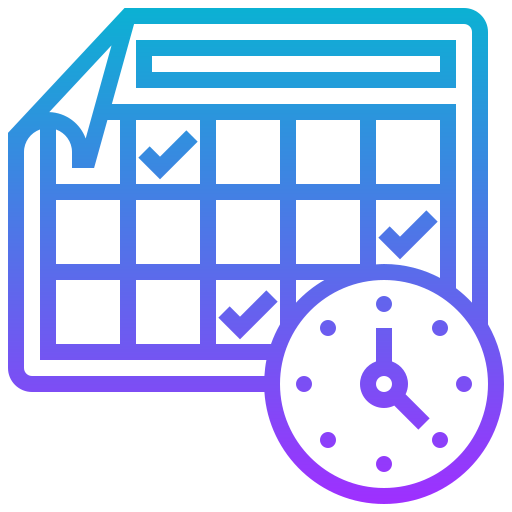
\includegraphics[width=2cm]{icono.png}
\end{center}
\end{figure}
\begin{Large}
\textbf{Agendaly} \\
\end{Large}
\begin{Med}
\textbf{Aplicación para la organización académica} \\
\end{Med}

\vspace*{3in}

\begin{large}
\raggedleft
\textbf{Autores:}Miguel Blanco Godón \\
Blanca Fernández Martín\\
Laura Cabezas González\\
\textbf{Fecha:}\textit{A Coruña, 15 de enero de 2022}\\
\end{large}

\end{center}
\end{titlepage} 

\newpage

\addtocontents{toc}{\hspace{-7.5mm} \textbf{Capítulos}}
\addtocontents{toc}{\hfill \textbf{Página} \par}
\addtocontents{toc}{\vspace{-2mm} \hspace{-7.5mm} \hrule \par}

\pagenumbering{empty}

\tableofcontents

\vspace{5cm}

\begin{flushright}
\begin{table}[hbtp]
\begin{center}

\caption{Tabla de versiones.}
\label{tabla:versiones}
\small
\vspace{1ex}

\begin{tabular}{|c|c|l|}
\hline
Versión & Fecha & Autor \\
\hline \hline
0.1 & 07/10/2021 & Grupo Q1.1 \\ \hline
0.2 & 09/11/2021 & Grupo Q1.1 \\ \hline
1.0 & 15/12/2021 & Grupo Q1.1 \\ \hline
1.5 & 15/01/2022 & Grupo Q1.1 \\ \hline
\end{tabular}

\end{center}
\end{table}
\end{flushright}


\newpage
\pagenumbering{arabic}


%%%%%%%
%%%%%%%
\section{Introducción}\label{cap.introduccion}

%%
\subsection{Objetivos}
El objetivo es la elaboración de una app de tipo agenda para organizar el estudio. Se podrán fijar fechas de entrega y exámenes de forma que se acceda a un calendario al que se puedan añadir eventos. También se podrá almacenar una copia del horario de clase en la aplicación, con información adicional de cada asignatura, como, por ejemplo, el aula en la que se imparte cada clase o el profesor. Se podrá entrar a la aplicación autenticándose mediante usuario y contraseña, y gracias a esto los usuarios registrados podrán organizarse en grupos, para sincronizar su forma de gestionar el estudio y repartir tareas entre ellos, de forma que cada miembro del grupo pueda marcar el estado en el que se encuentra la parte de la tarea en la que esta trabajando (si está trabajando todavía en ella, si está terminada, etc.) y el resto de integrantes puedan verlo. La aplicación también podrá acceder al reloj y podrá fijar recordatorios o alarmas en función de la hora, de forma que pueda avisar al usuario de que un día en concreto a partir de una hora determinada ha planeado que se tiene que poner a estudiar. Desde la aplicación también será posible compartir los documentos de los trabajos en grupo en la nube, y descargarlos para tener una copia y acceder a ellos sin conexión.
Se utilizará GitHub para el control de versiones de nuestra app. \cite{misc-git}
%%
\subsection{Motivación}
La buena gestión del tiempo es un aspecto básico para la consecución de un curso escolar. Por ese motivo necesitamos un mecanismo de gestión que nos ayude a mejorar nuestra producción académica con el menor esfuerzo posible, a través de un sistema sencillo, fácil de manejar, con control automático y centralizado que nos informe sobre los detalles de las diferentes tareas. 
Esta gestión se vuelve crítica cuando las tareas a realizar son grupales, especialmente si los integrantes tienen diferentes horarios. En este caso, un sistema de sincronización de tareas con recursos compartidos el cual monitorizase y notificara las tareas hechas y venideras a los diversos integrantes sería muy útil.
%%
\subsection{Trabajo relacionado}
Aplicaciones relacionadas con partes de nuestra app:
- TimeTune es una aplicación de gestión de tiempo y planificador de horarios \cite{misc-url1}

Reminder es una apps para recordatorios, alarmas y tareas. \cite{misc-url2}

Exam-countdown es una app para realizar un seguimiento de los exámenes y pruebas fechas.\cite{misc-url3}

Además también nos inspira mucho a la hora de saber las entregas la propia interfaz de moodle, ya que nos va indicando las entregas y su fecha límite.

%%%%%%%
%%%%%%%
\section{Análisis de requisitos}

%%
\subsection{Funcionalidades}
Las funcionalidades principales serán:
\begin{itemize}
\item \textbf{1.Fijar fechas en el calendario [feature/calendar]:} desde la aplicación habrá una forma de establecer citas que se crearán en un calendario. Se podrá fijar la fecha, el nombre del evento, y alguna nota informativa a mayores. La aplicación llevará una agenda donde se mostrarán ordenadamente los eventos creados y sus fechas. Además, el usuario podrá eliminar un evento cuando considere.

\item \textbf{2.Almacenar el horario de clases [feature/horario]:} se podrá crear un horario semanal introduciendo las asignaturas y algún atributo a mayores, por ejemplo, el aula en la que se imparte y la hora . El horario será visible nada más abrir la aplicación.

\item \textbf{3.Autenticación[feature/authentication]:} el usuario podrá identificarse al entrar en la app, de forma que pueda acceder a sus datos desde otros dispositivos. Además, la autenticación del usuario verifica su identidad frente a otros usuarios a la hora de trabajar en grupos.

\item \textbf{4.Notificaciones de horario[feature/horario]:} el usuario podrá escoger si quiere que le notifique el horario diariamente y la hora a la que quiere que se produzca esa notificación.

\item \textbf{5.Notificaciones de calendario[feature/calendar]:} al crear un evento, el usuario podrá decidir si quiere que se le avise de ese evento mediante una notificación, y en caso de que así sea, podrá decidir la antelación con la que quiere ser avisado. Además, podrá modificar cuando se le envía la notificación o desactivarla en cualquier momento.


\end{itemize}

Y las funcionalidades secundarias serán:
\begin{itemize}

\item \textbf{Grupos de trabajo:} se podrán establecer tareas conjuntas para los integrantes de un grupo, y cada integrante podrá ir actualizando el avance de su trabajo de forma pública para el resto de sus compañeros.

\item \textbf{Apuntes en la nube:} el usuario podrá acceder a archivos que hayan compartido otros usuarios de a los que pertenezca. Será posible descargar estos documentos para poder acceder sin conexión. 
\end{itemize}

%%
\subsection{Prioridades}
El objetivo principal de esta aplicación es implementar de forma simple las funcionalidades de una agenda, aprovechando las comodidades que puede aportar un teléfono móvil. Es por esto que las prioridades serán las tareas más cercanas a la funcionalidad de la agenda, es decir, fijar las fechas de los eventos importantes en un calendario y mantener una copia fácilmente accesible del horario semanal. 



%%%%%%%
%%%%%%%
\section{Planificación inicial}

%%
\subsection{Iteraciones}
Se harían cuatro iteraciones incrementales. En la primera, se intentará que la aplicación tenga su funcionalidad básica: horario, gestión de calendario y usuarios.
En la segunda iteración se haría la extensión multiusuario y notificación: notificaciones, creación de grupos y sincronización básica de tareas. También se corregirían errores de la iteración anterior.
En la tercera iteración se añadirá el repositorio de datos común y la gestión comunal de tareas. También se corregirán los errores de la iteración anterior.
En la iteración final, se corregirán los fallos de las iteraciones anteriores y se hará la integración final de conjunto.

%%
\subsection{Responsabilidades}
Se llevará a cabo la implementación de tres funcionalidades simultáneamente, para que todos los miembros del grupo puedan trabajar simultáneamente sin tener que esperar a por el trabajo de los demás. Las primeras funcionalidades a implementar se repartirán tal que 
la creación del calendario será implementada por Blanca Fernández, el horario semanal por Laura Cabezas y la autenticación por Miguel Blanco. 
\newline
La creación y gestión de equipos será responsabilidad de Miguel Blanco. La funcionalidad de añadir notificaciones al horario será responsabilidad de Laura Cabezas. Y la posibilidad de añadir notificaciones al calendario será responsabilidad de Blanca Fernández.
%%
\subsection{Hitos}
Se realizará una entrega por cada funcionalidad implementada, más otras dos a mayores, al final de cada iteración, donde se solucionarán los detalles de integración de las partes en las que se dividió el trabajo. Por lo tanto, habrá tres hitos iniciales para las tres funcionalidades ya repartidas, y un cuarto hito donde se mostrará una primera versión funcional de la aplicación, aunque con funcionalidades reducidas. Más adelante, volverá a haber un hito por cada funcionalidad secundaria que se implemente, y finalmente, la entrega final de la aplicación completa.

%%


%%%%%%%
%%%%%%%
\section{Diseño}

%%
\subsection{Arquitectura}
Para esta aplicación vamos a usar el patrón de arquitectura Clean.

\subsection{Persistencia}
Para la persistencia de usuarios se utilizarán ficheros de shared preferences almacenados en local. Por seguridad, las contraseñas estarán cifradas. Los eventos de calendario/horario se guardarán en una base de datos de Firebase. Para guardar los datos usaremos dos bases de datos implementadas con Room, una para el calendario y otra para el horario.
Para la persistencia de contactos y equipos, se usará una base de datos local (ROOM) que servirá para acceder a la información a modo de consulta cuando los usuarios pierdan la conexión internet (es necesaria la conexión para acceder a la app puesto que hay que llevar a cabo un proceso de autenticación). También se dispondrá de una base de datos documental en un ambiente cloud (Firestore) que permitirá mantener la persistencia de estos datos asociada a la cuenta de los usuarios, permitiendo la recuperación automática de la información en caso de que los usuarios cambien de dispositivo.

\subsection{Vista}
Ver figuras 1, 2, 3,4 y 5.
\begin{figure}
            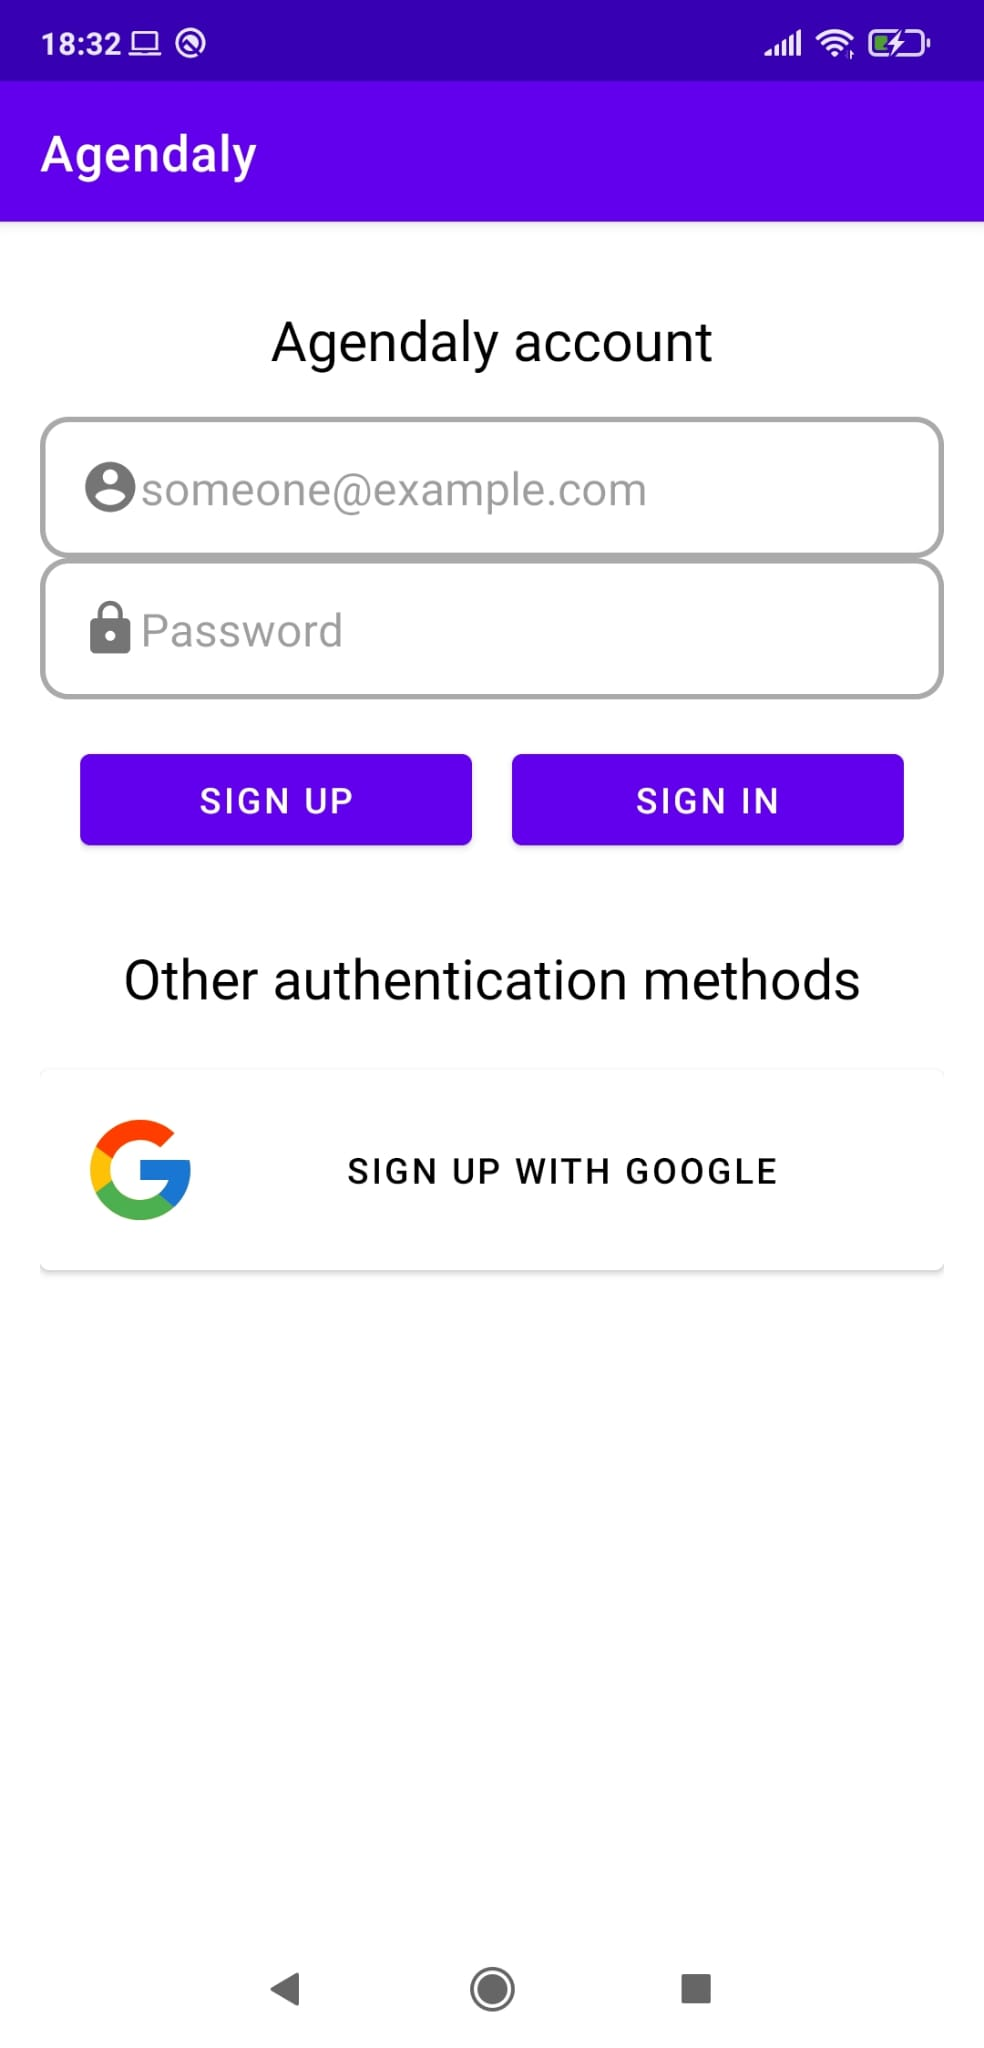
\includegraphics[scale=0.05]{view.jpeg} \hfill
            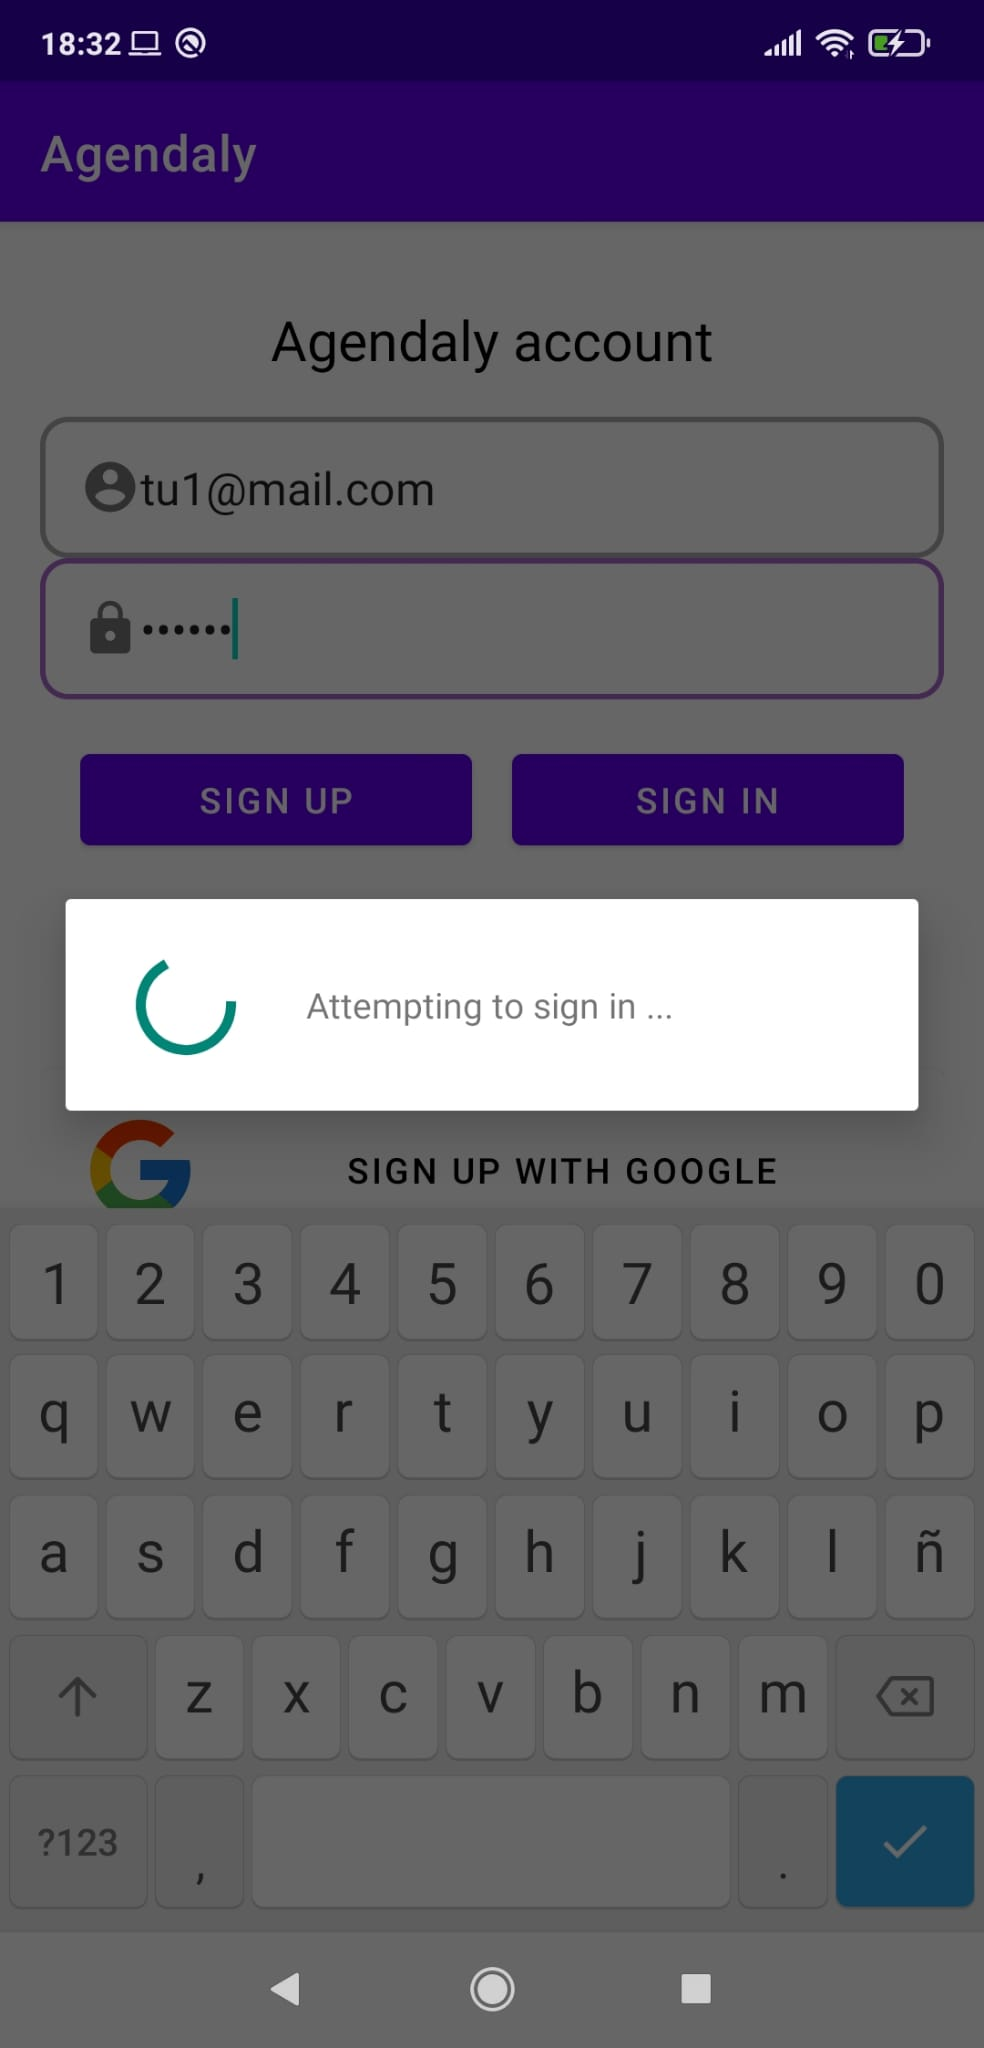
\includegraphics[scale=0.05]{dialog.jpeg}\hfill
            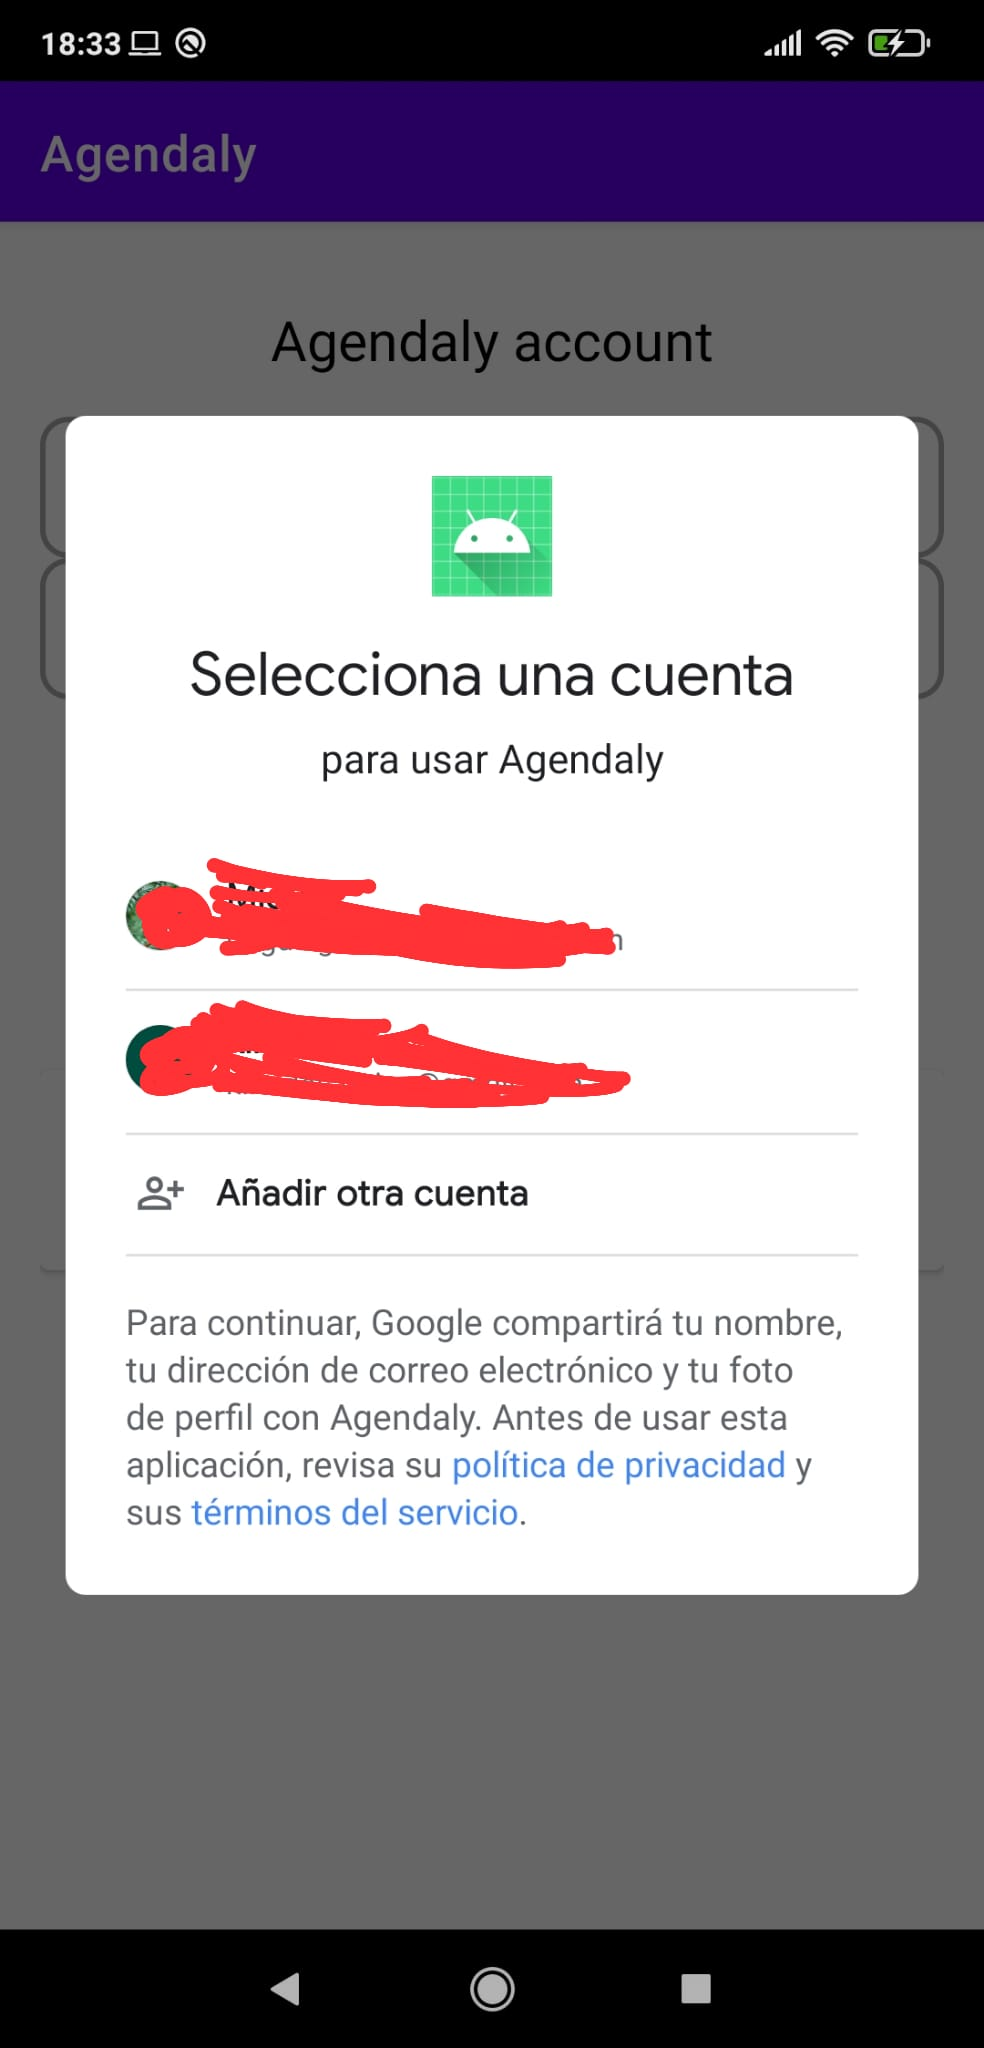
\includegraphics[scale=0.05]{google.jpeg} \hfill
            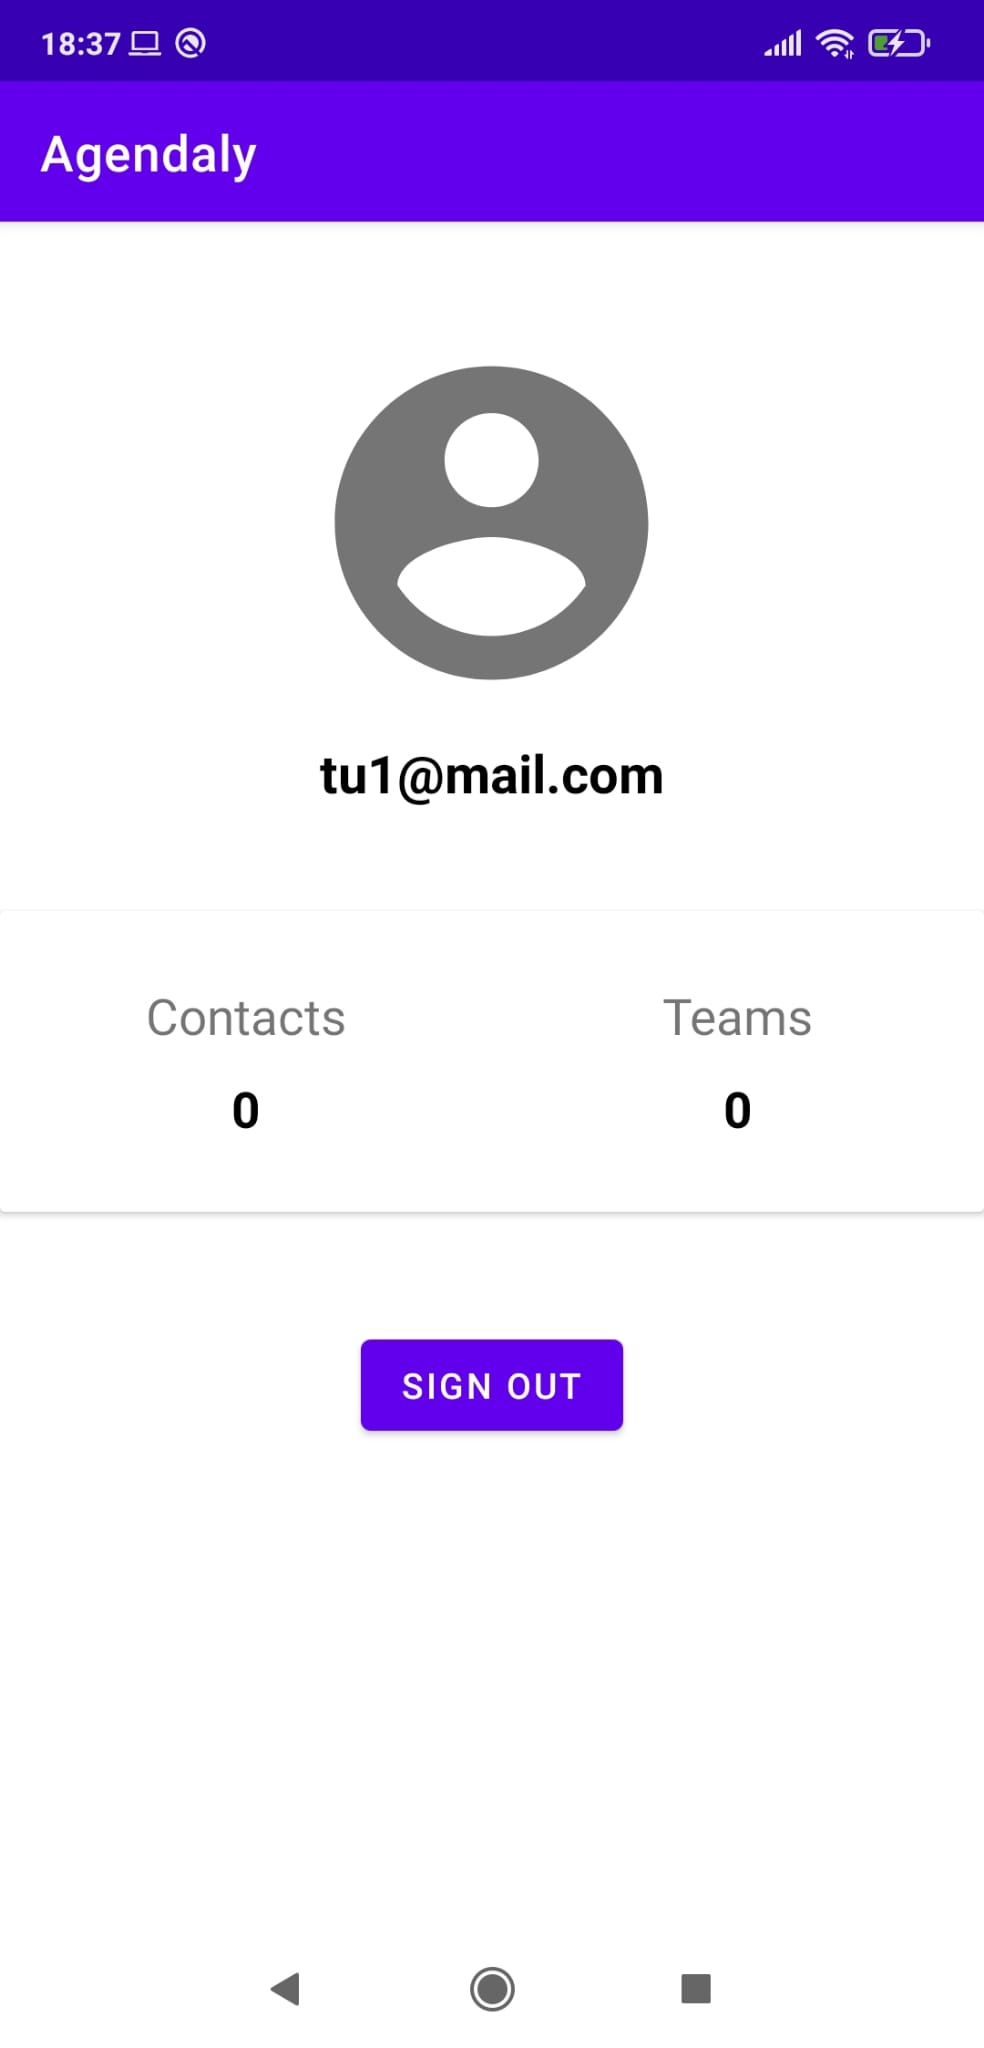
\includegraphics[scale=0.05]{account_view.jpeg}
            \caption{Pantallas de autenticación}
        \end{figure}

\begin{figure}
            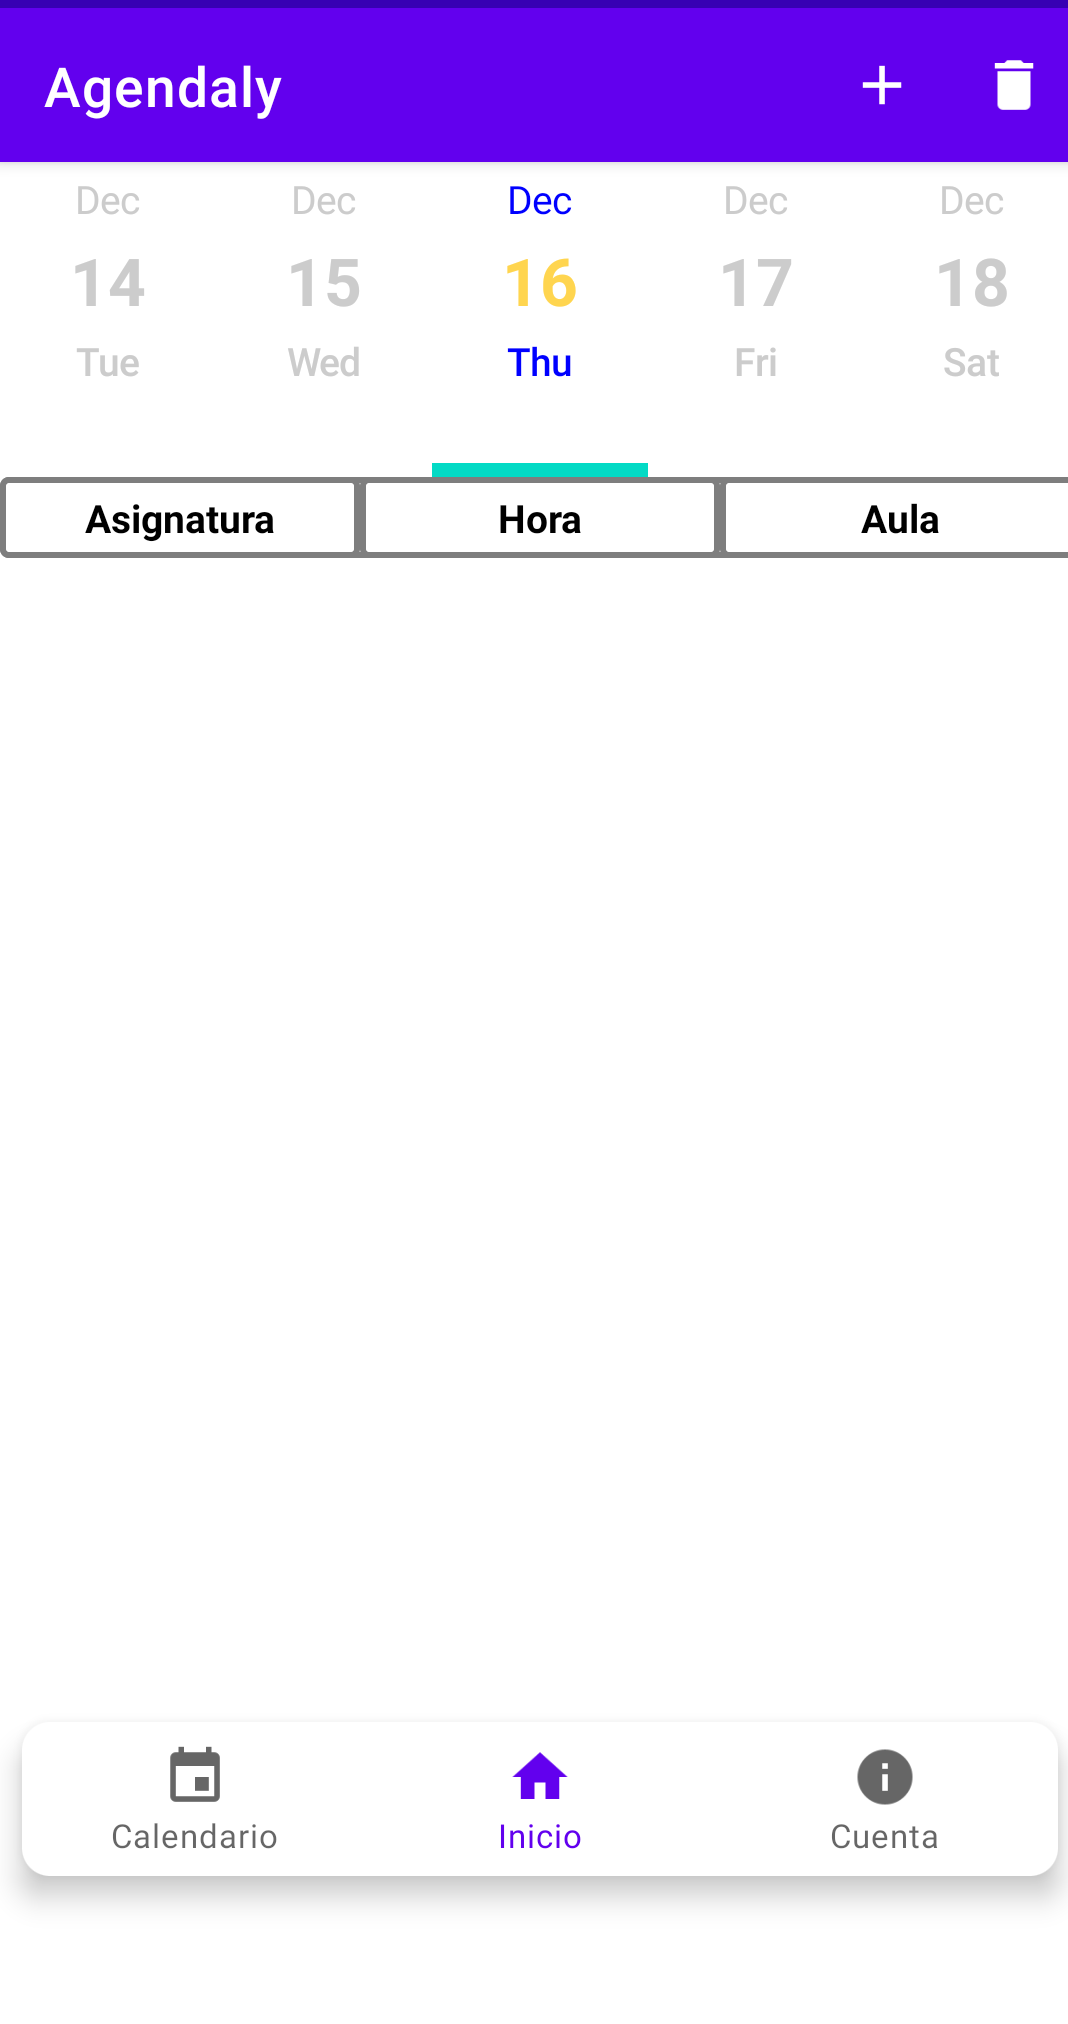
\includegraphics[scale=0.05]{Horario.png} 
            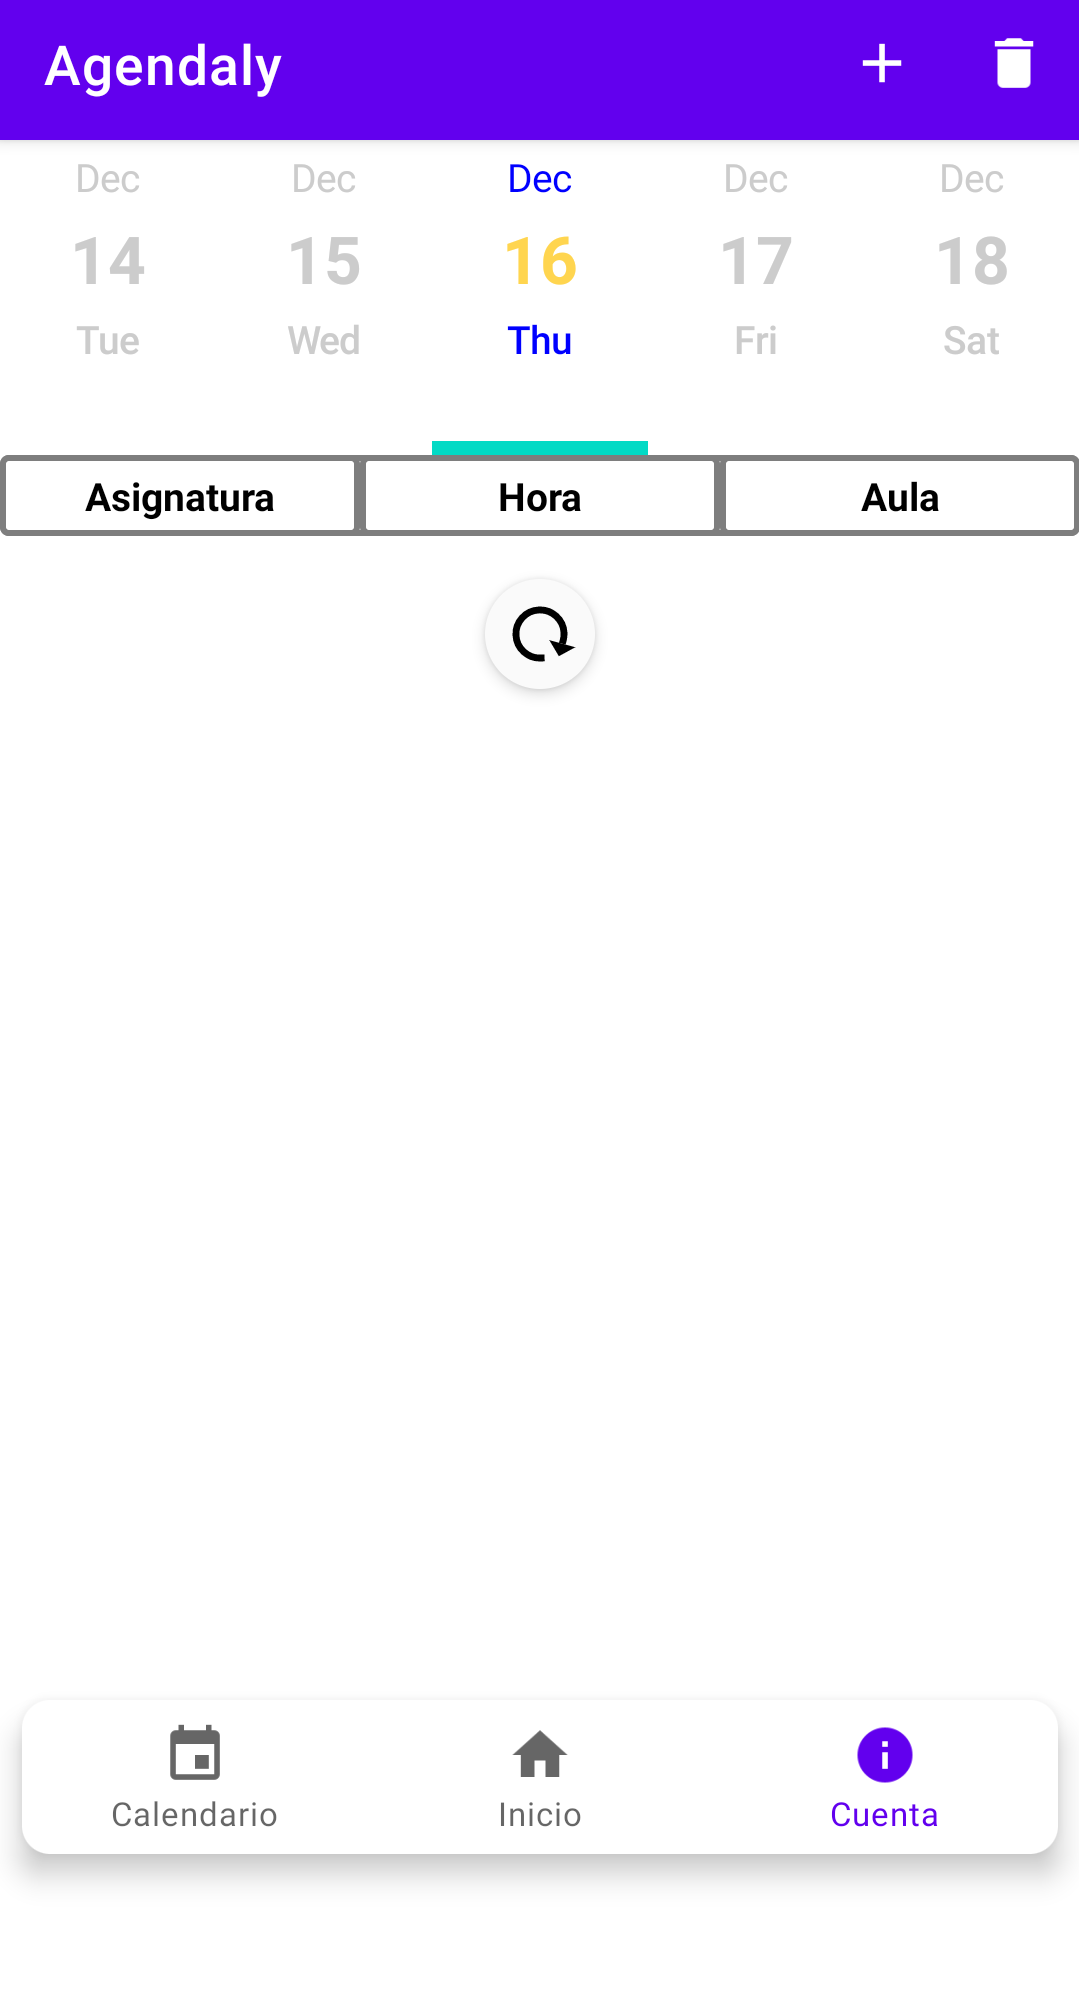
\includegraphics[scale=0.05]{swipe.png}\hfill
            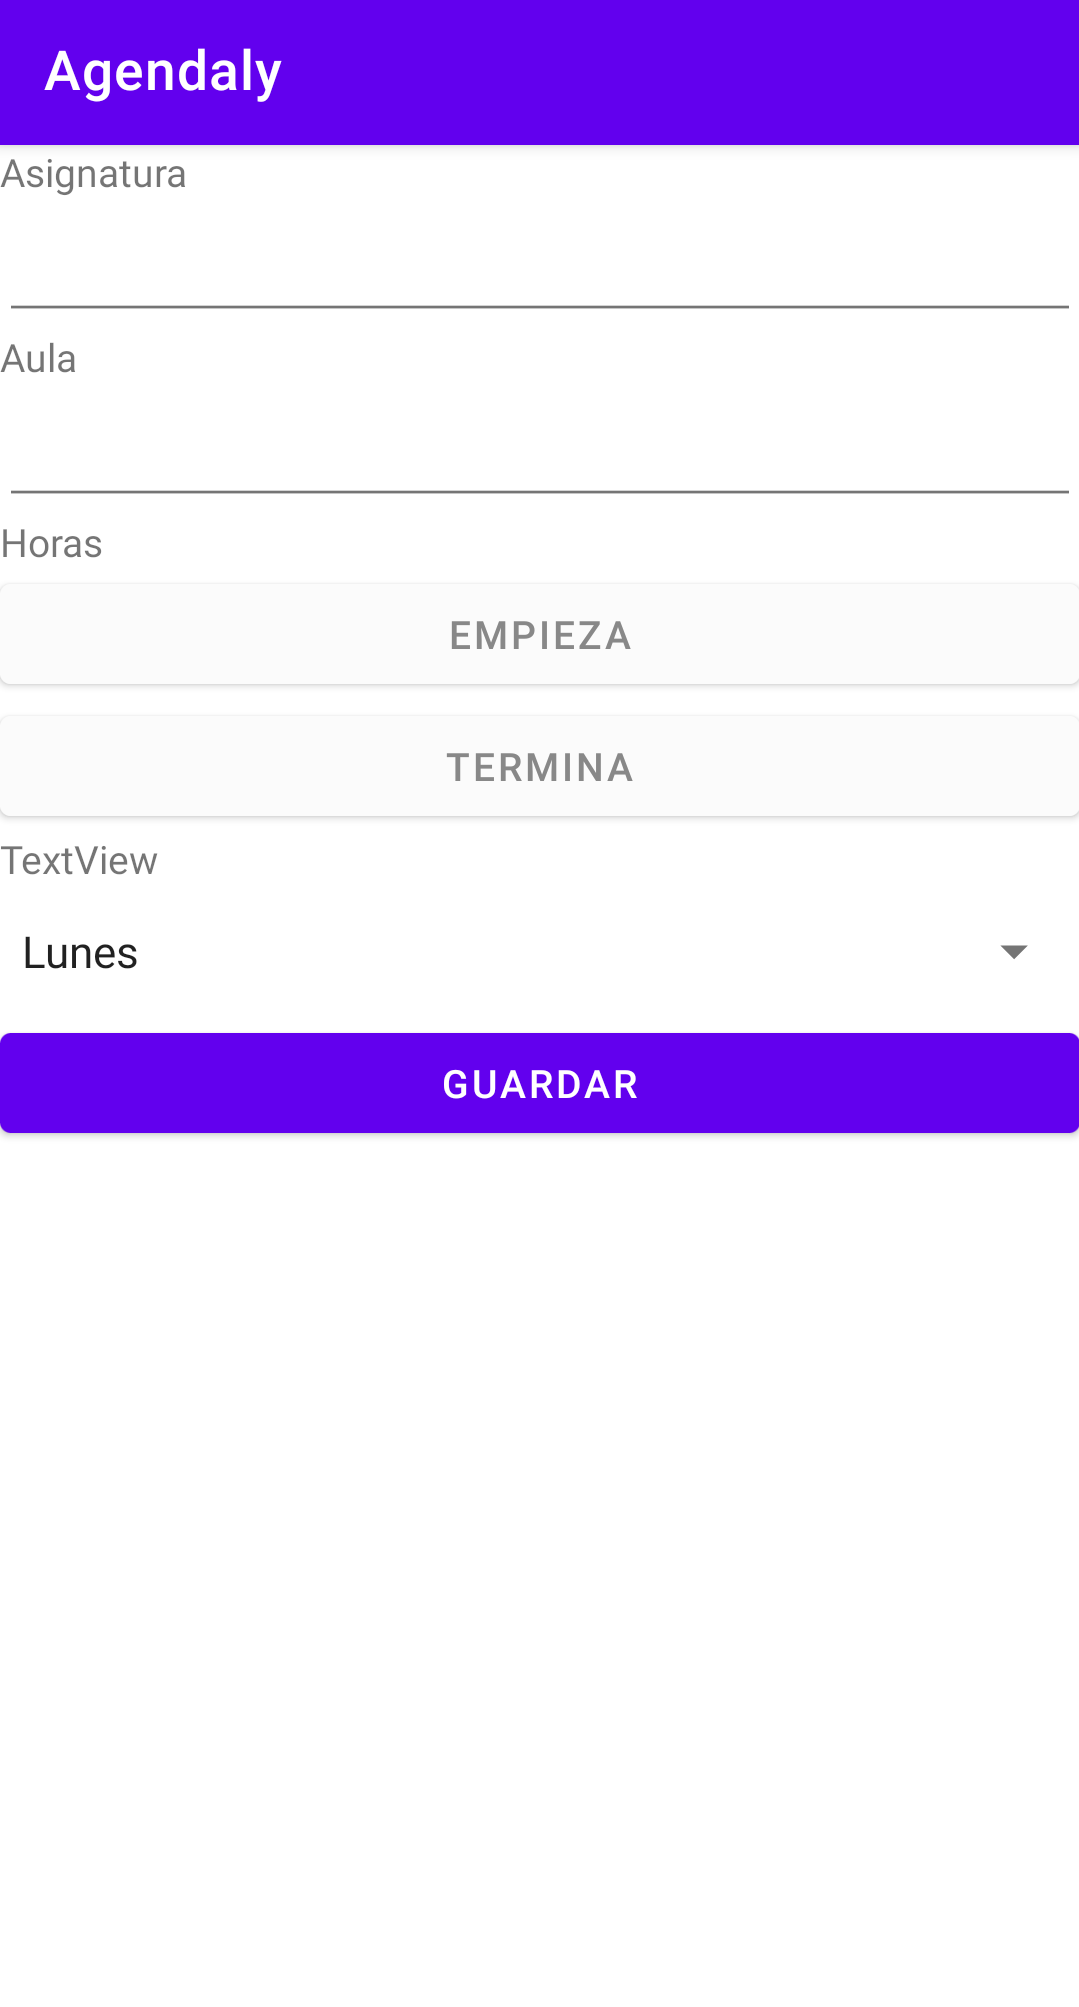
\includegraphics[scale=0.05]{Add.png} 
            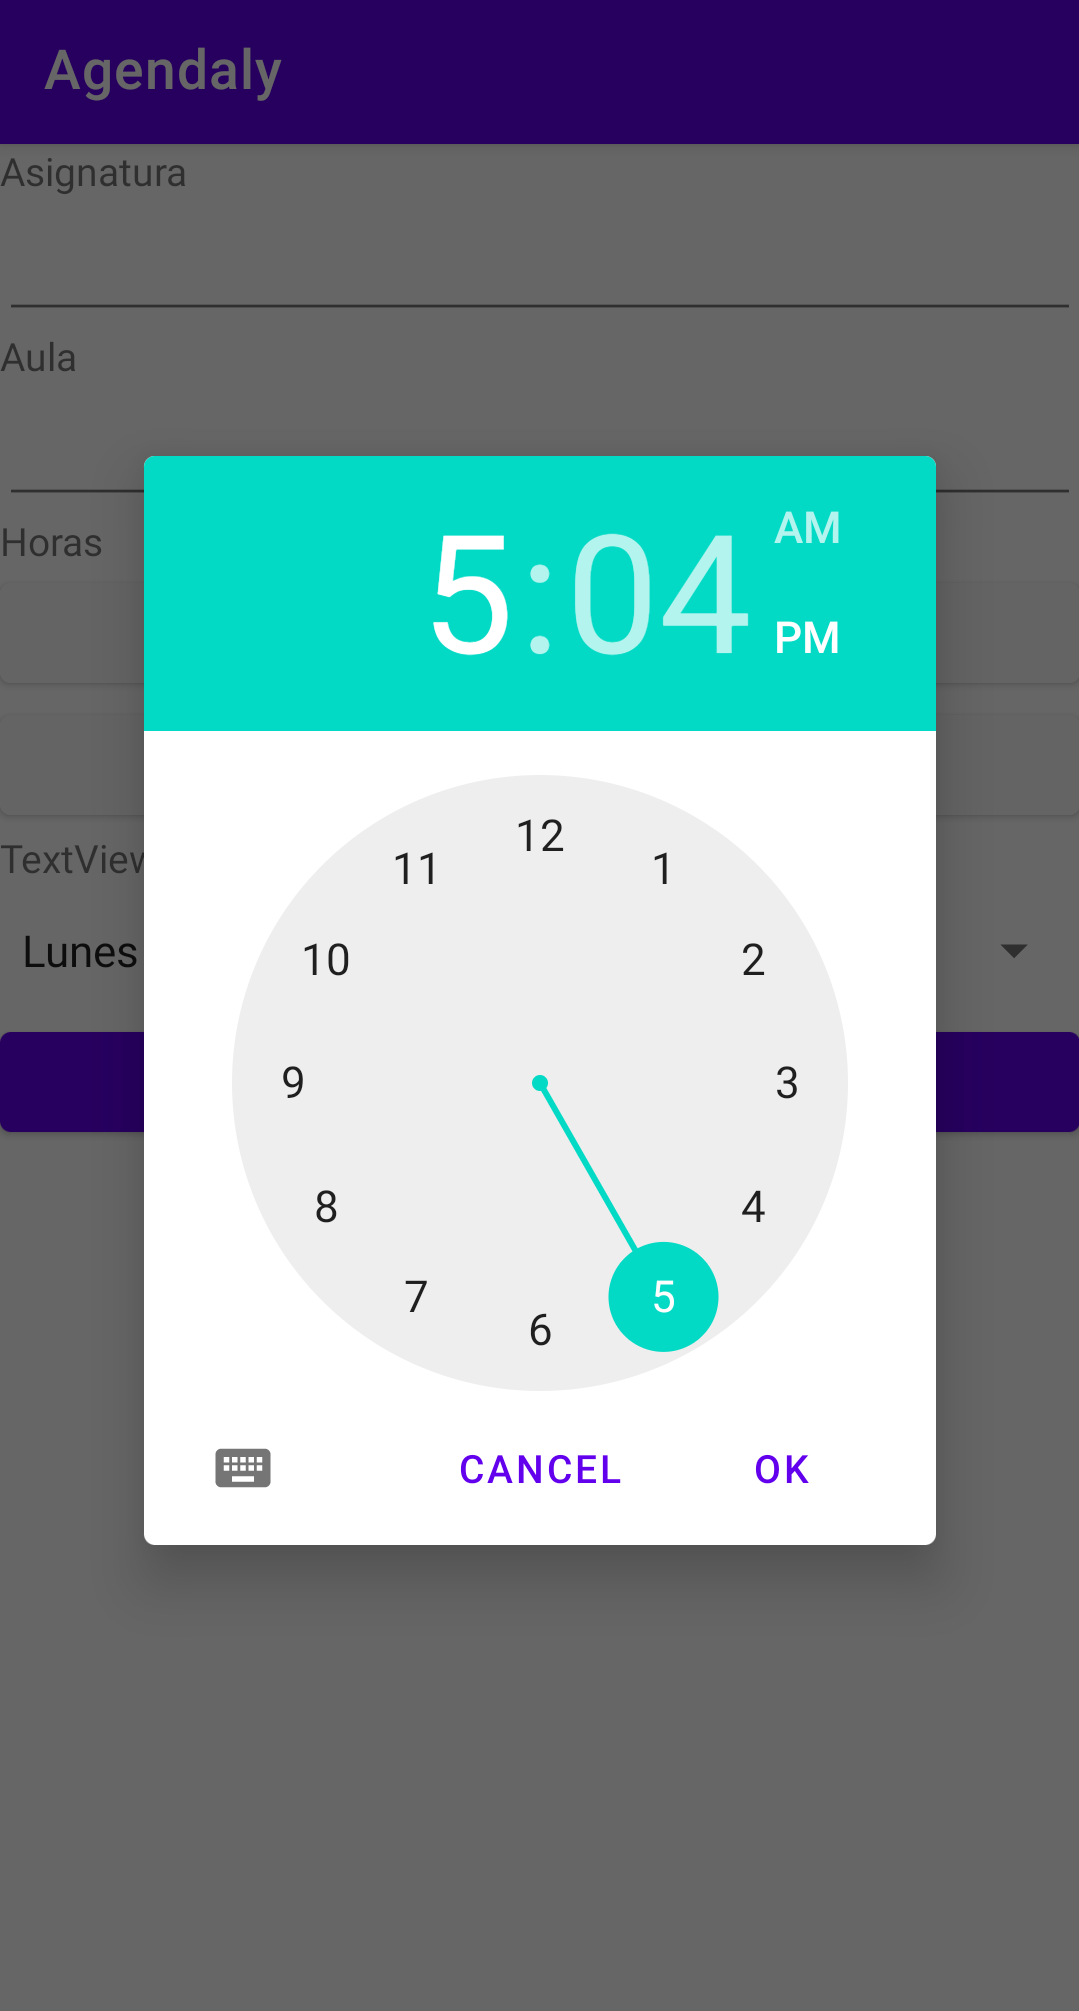
\includegraphics[scale=0.05]{add_timepicker.png}
            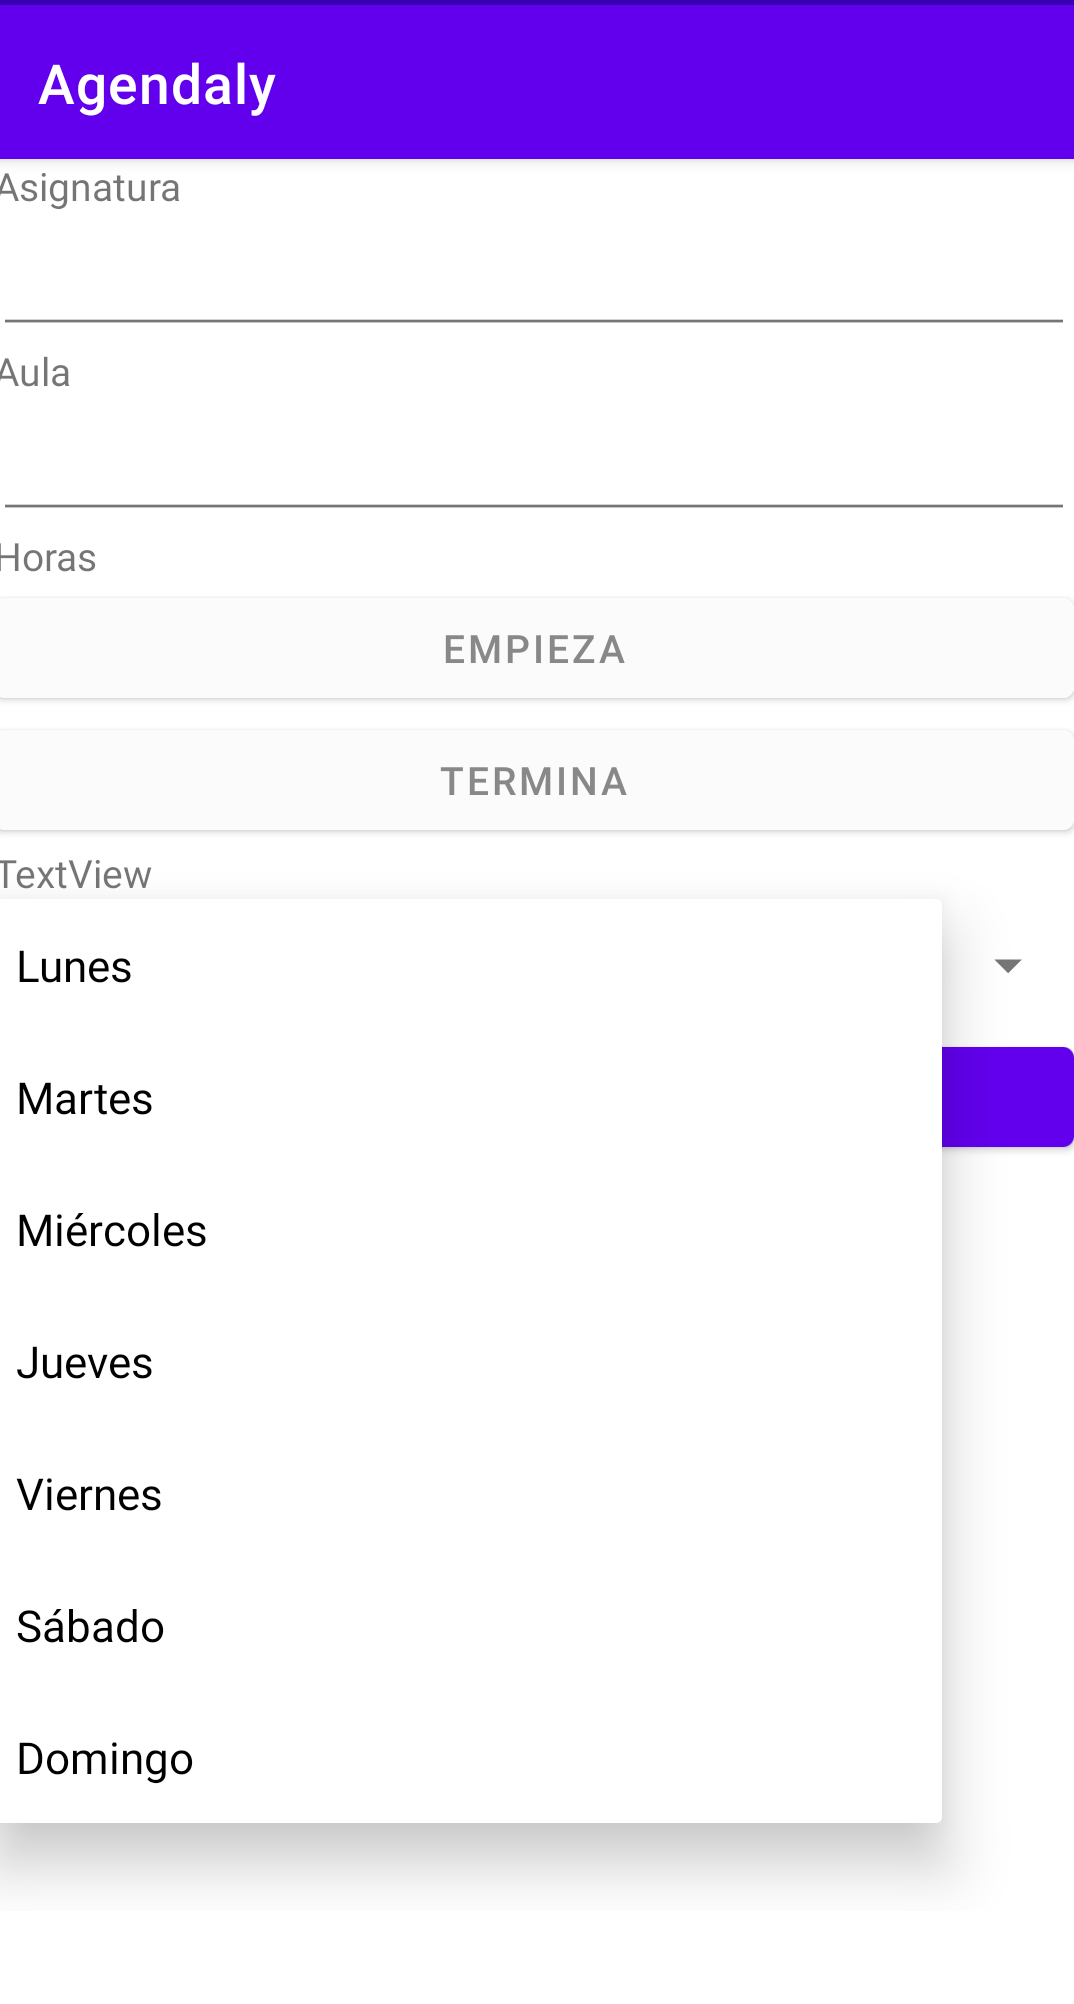
\includegraphics[scale=0.05]{add_spinner.png}
            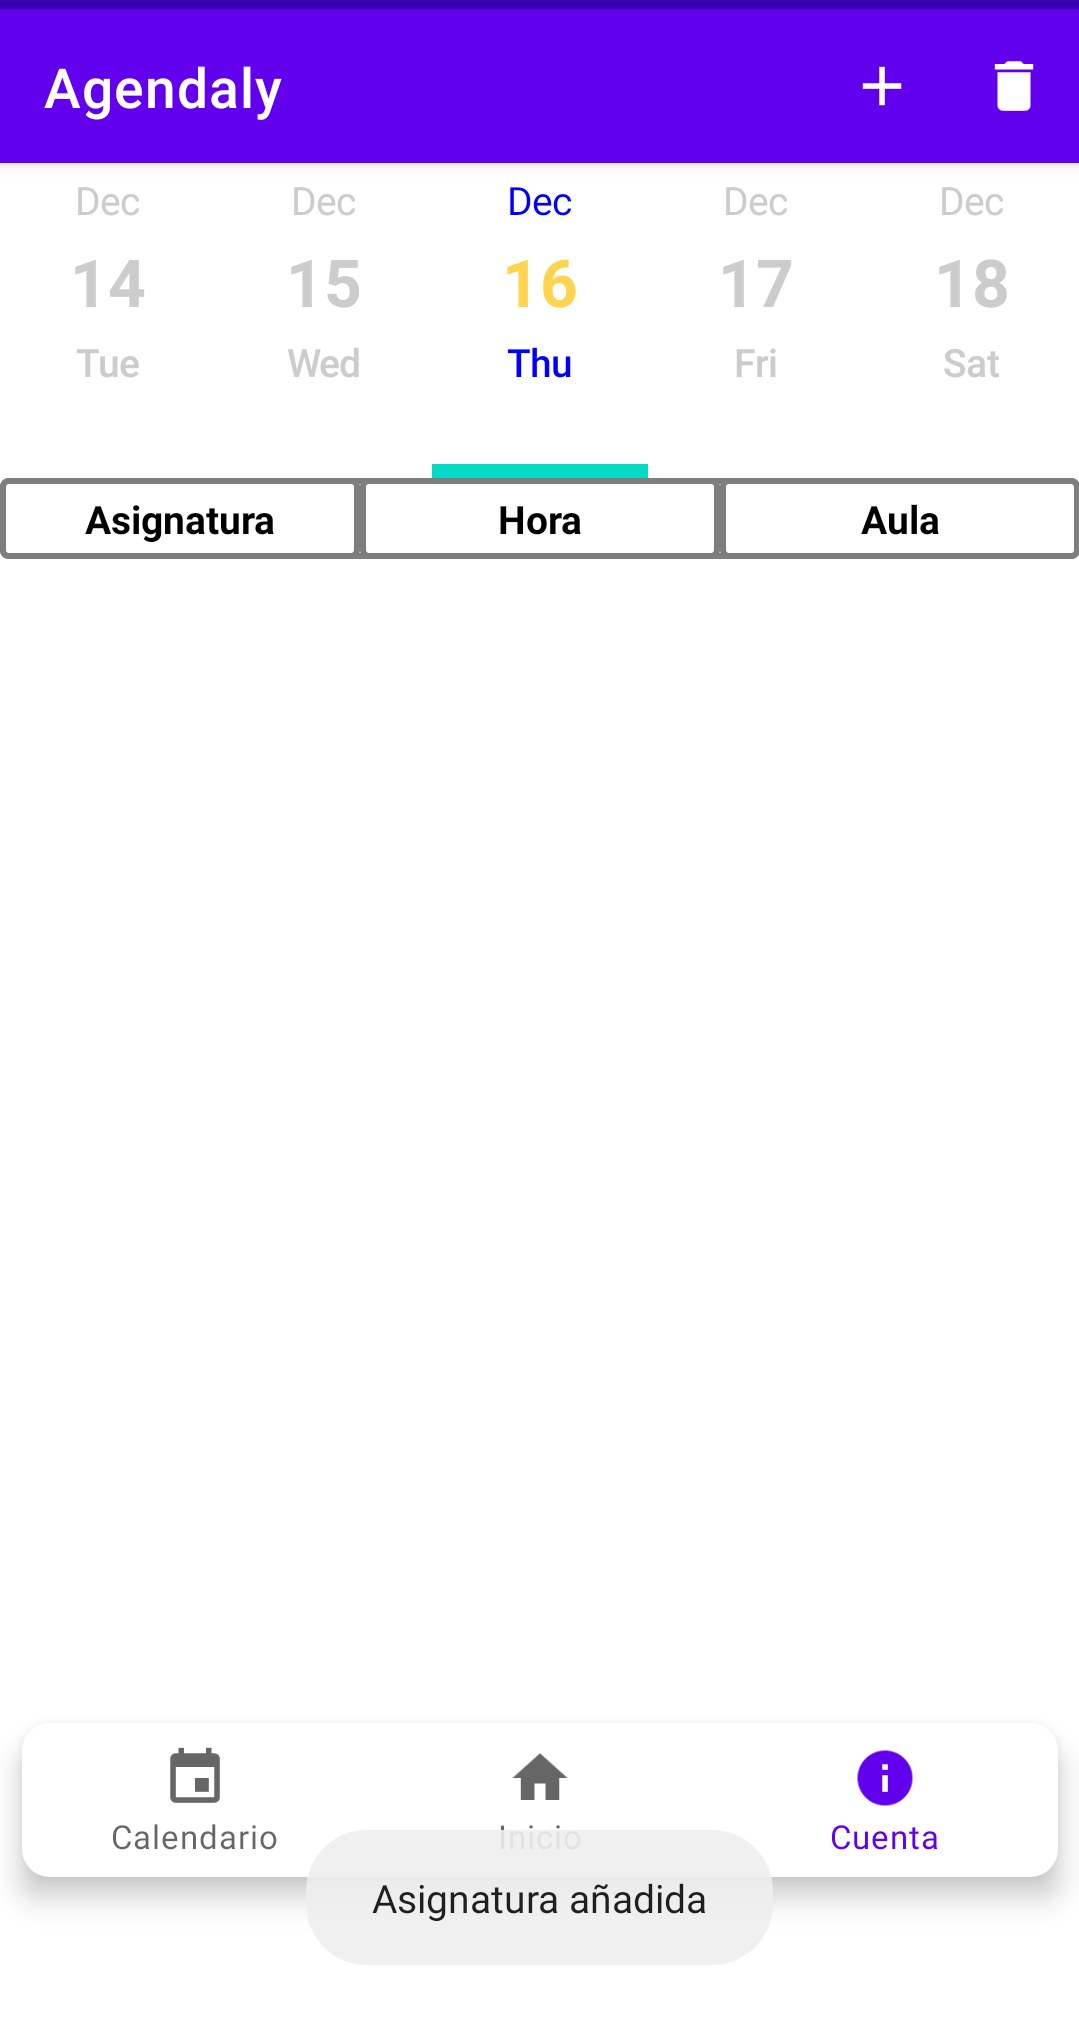
\includegraphics[scale=0.05]{ToastAdd.png}\hfill
            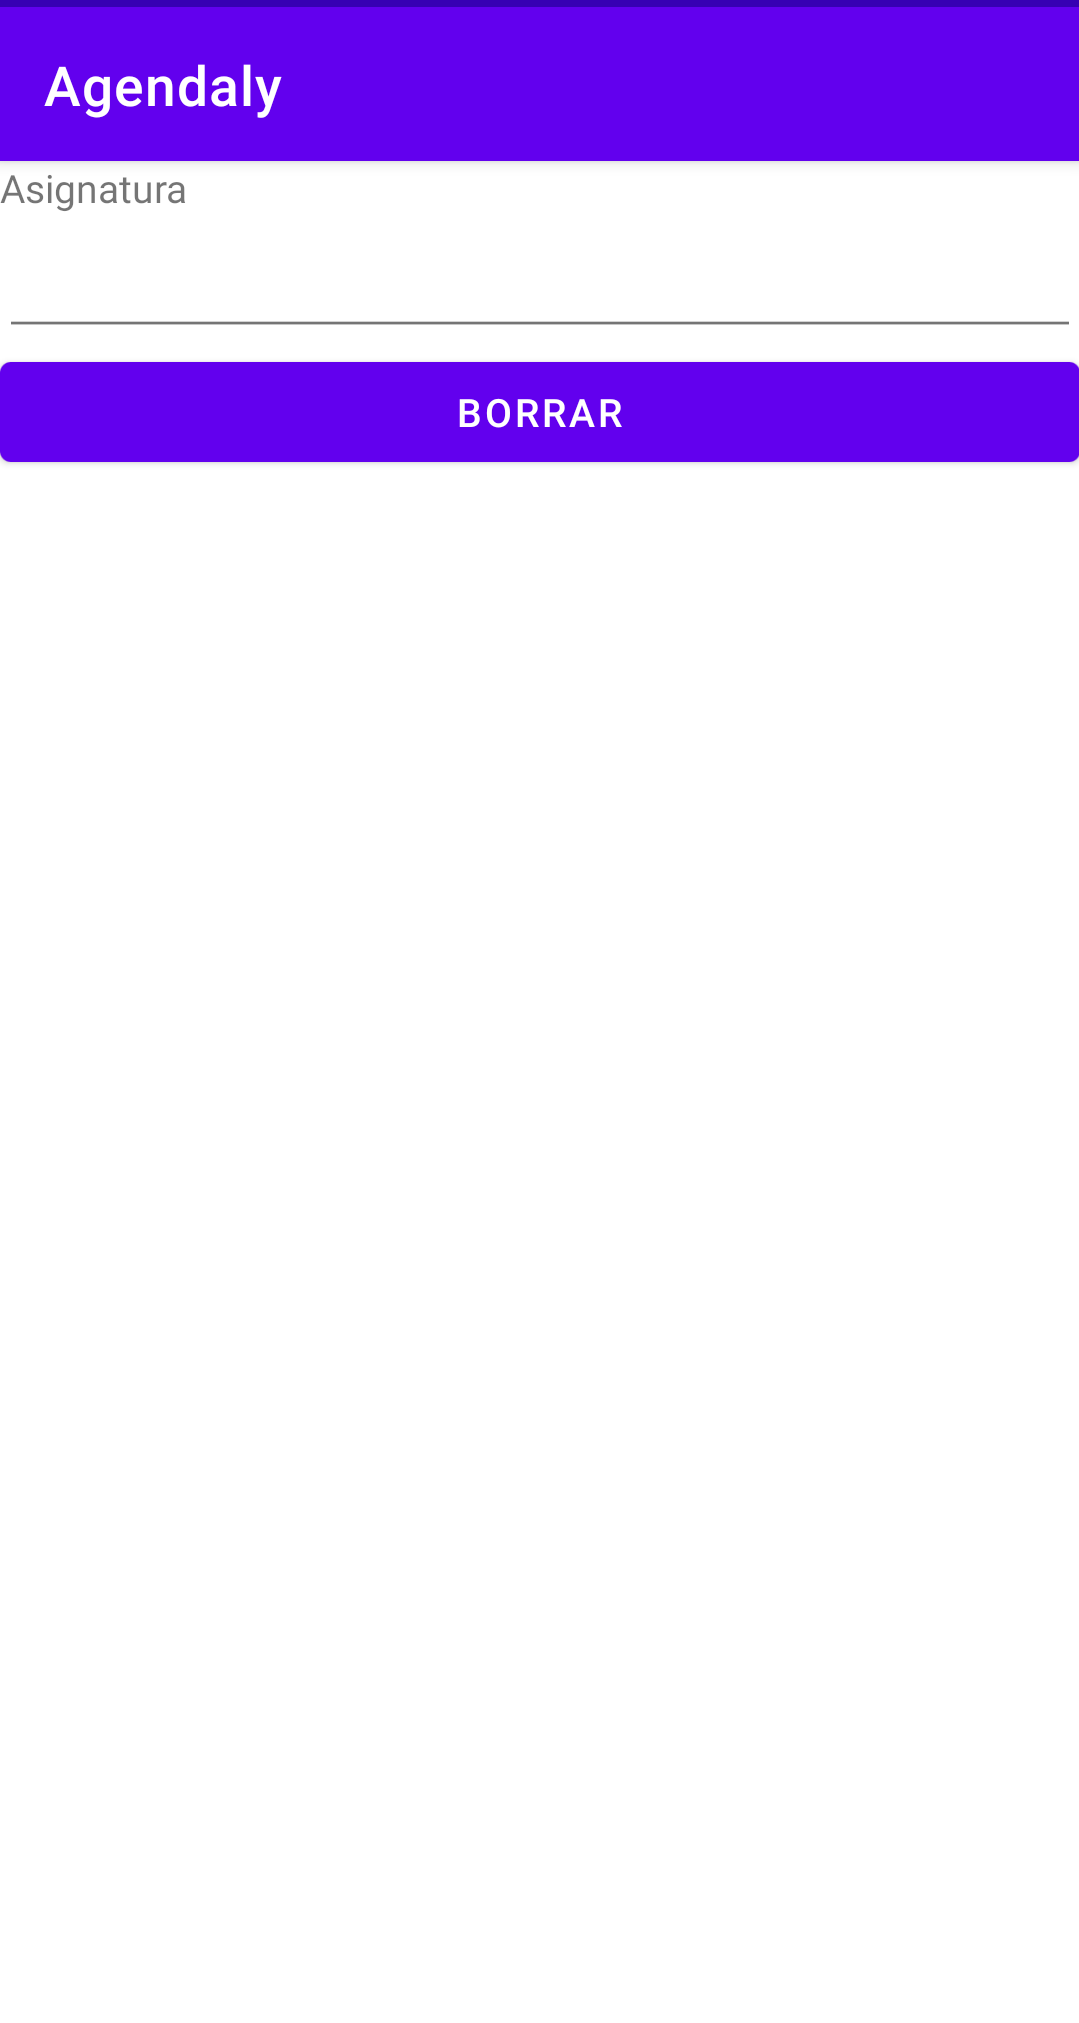
\includegraphics[scale=0.05]{borrar.png}
            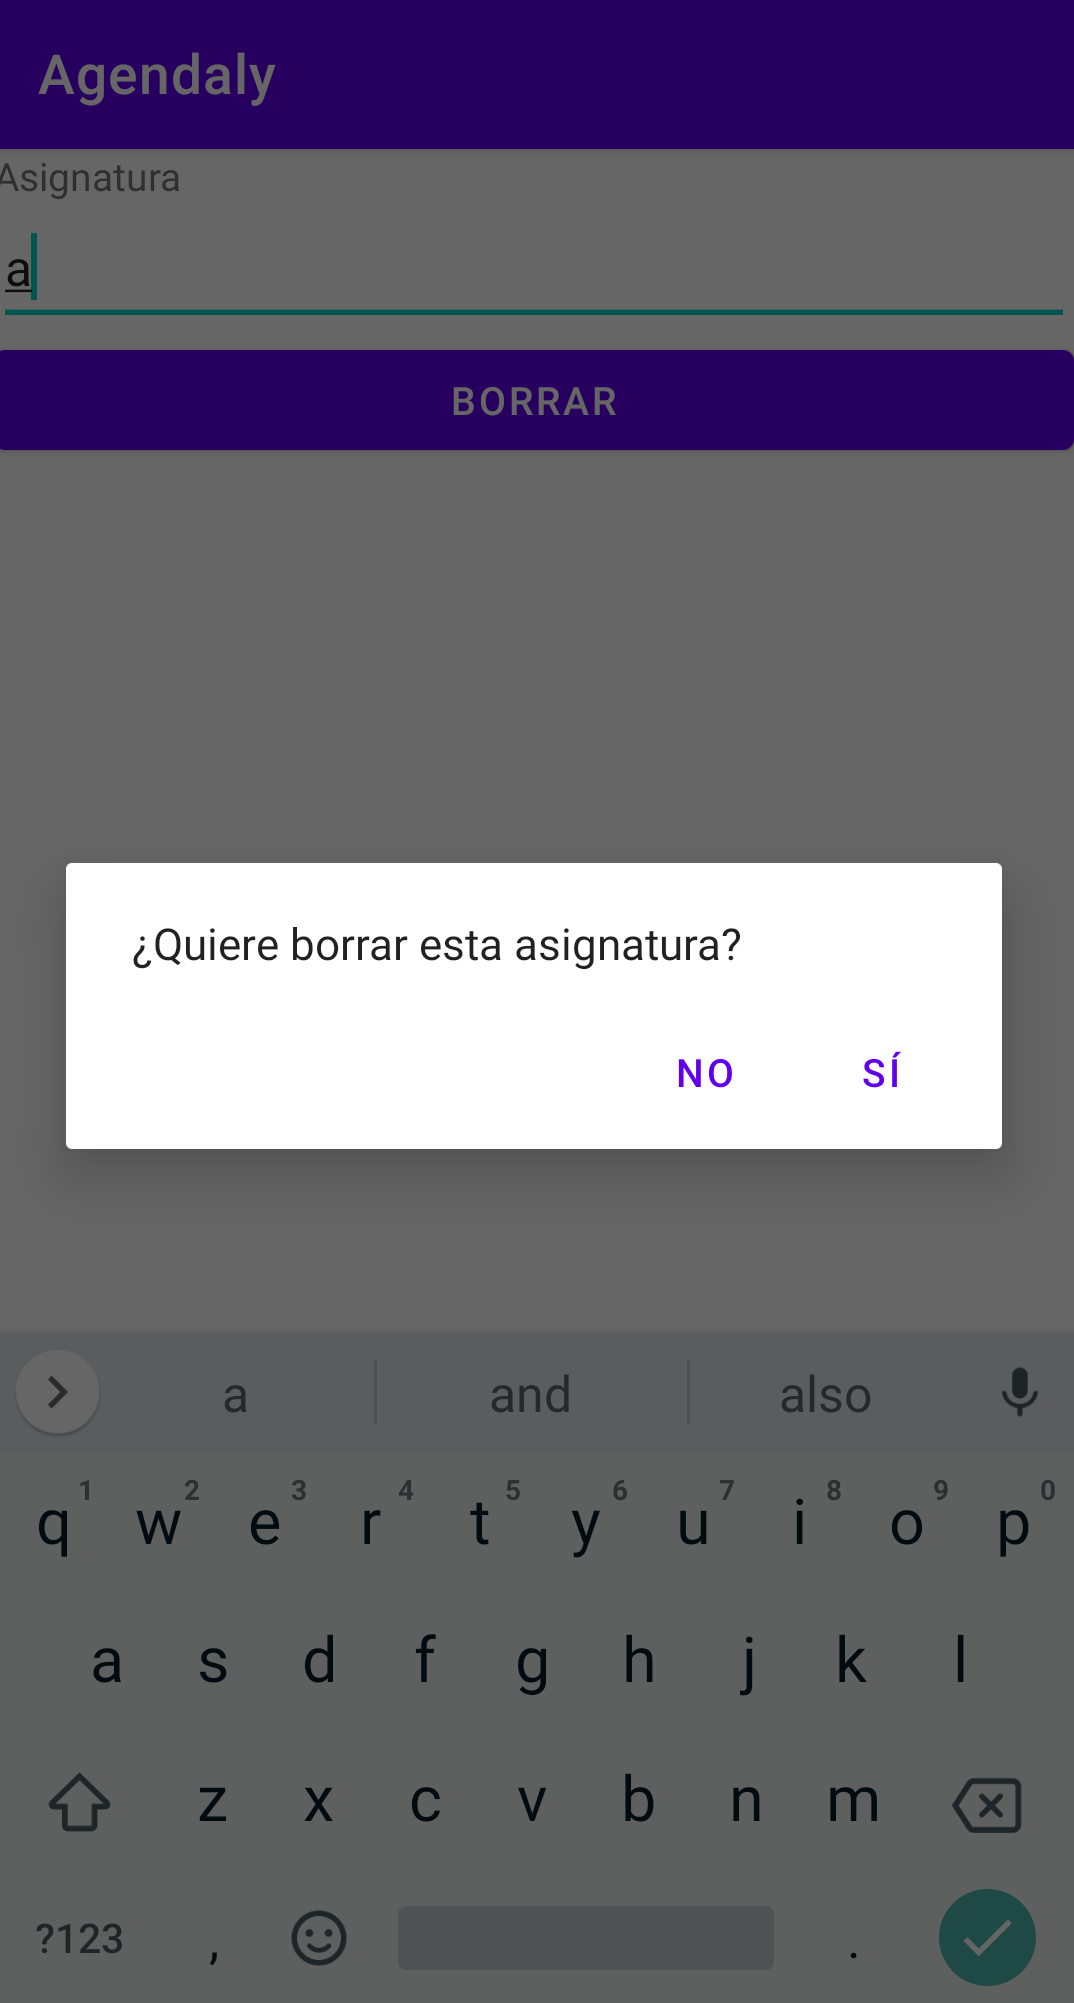
\includegraphics[scale=0.05]{avisoBorr.png}
            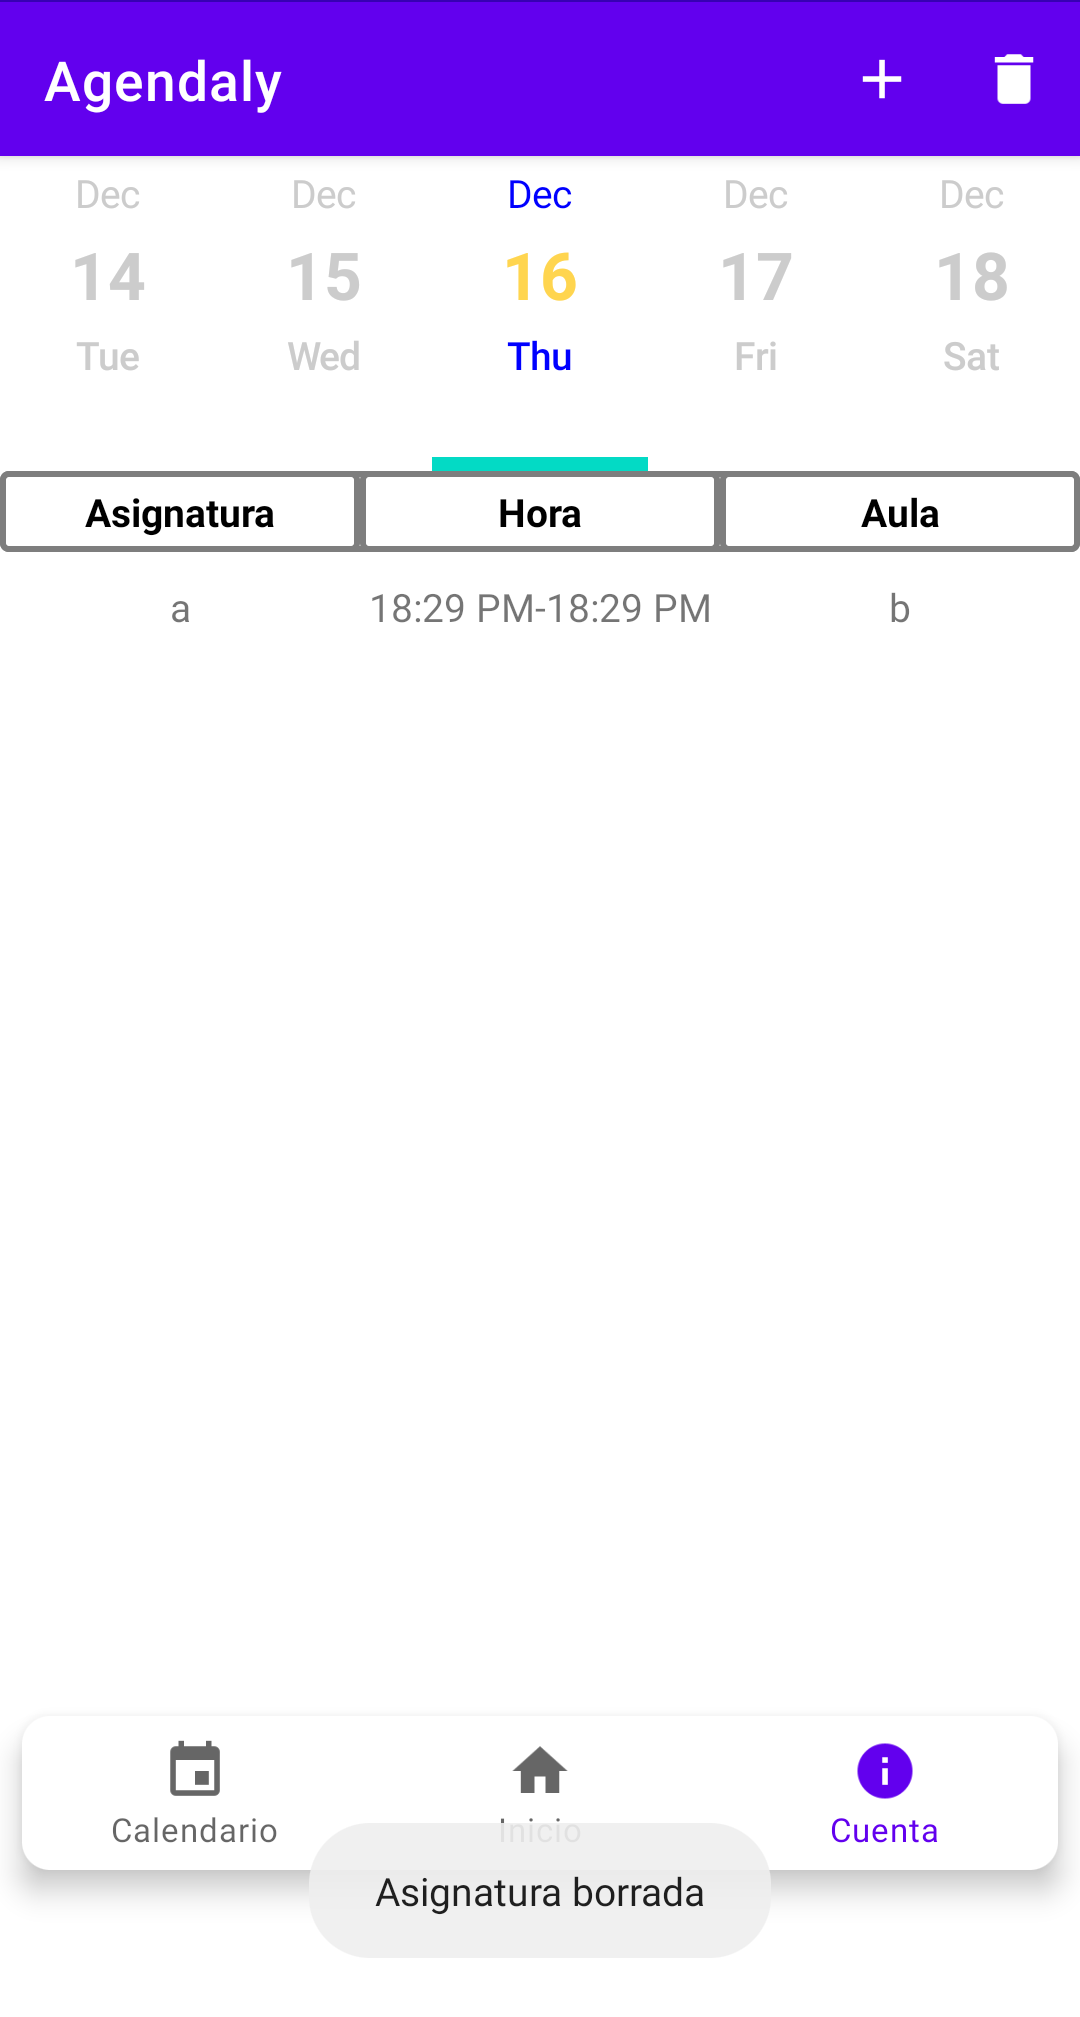
\includegraphics[scale=0.05]{asignaturaBorrToast.png}
            \caption{Pantallas del horario}
        \end{figure}
        
\begin{figure}
        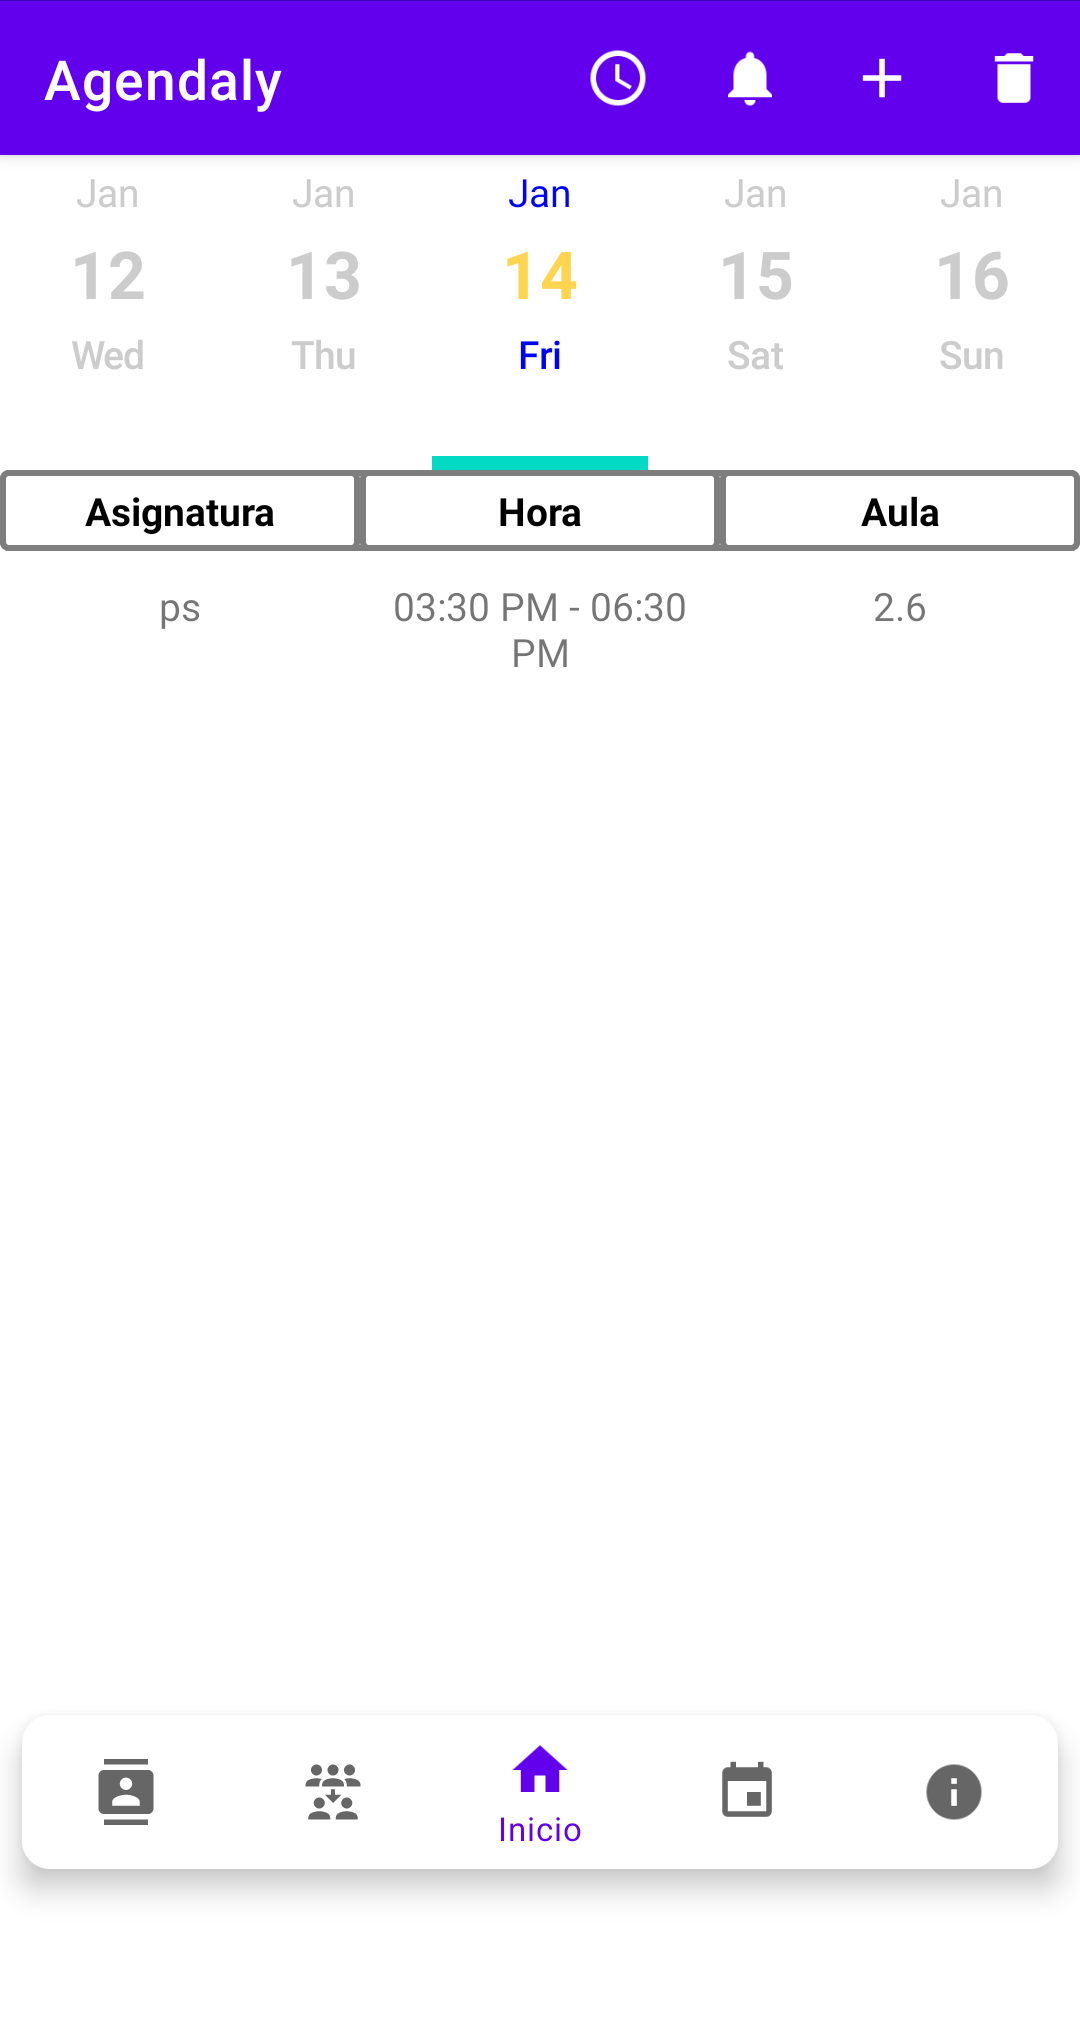
\includegraphics[scale=0.05]{notificacion1.png} 
        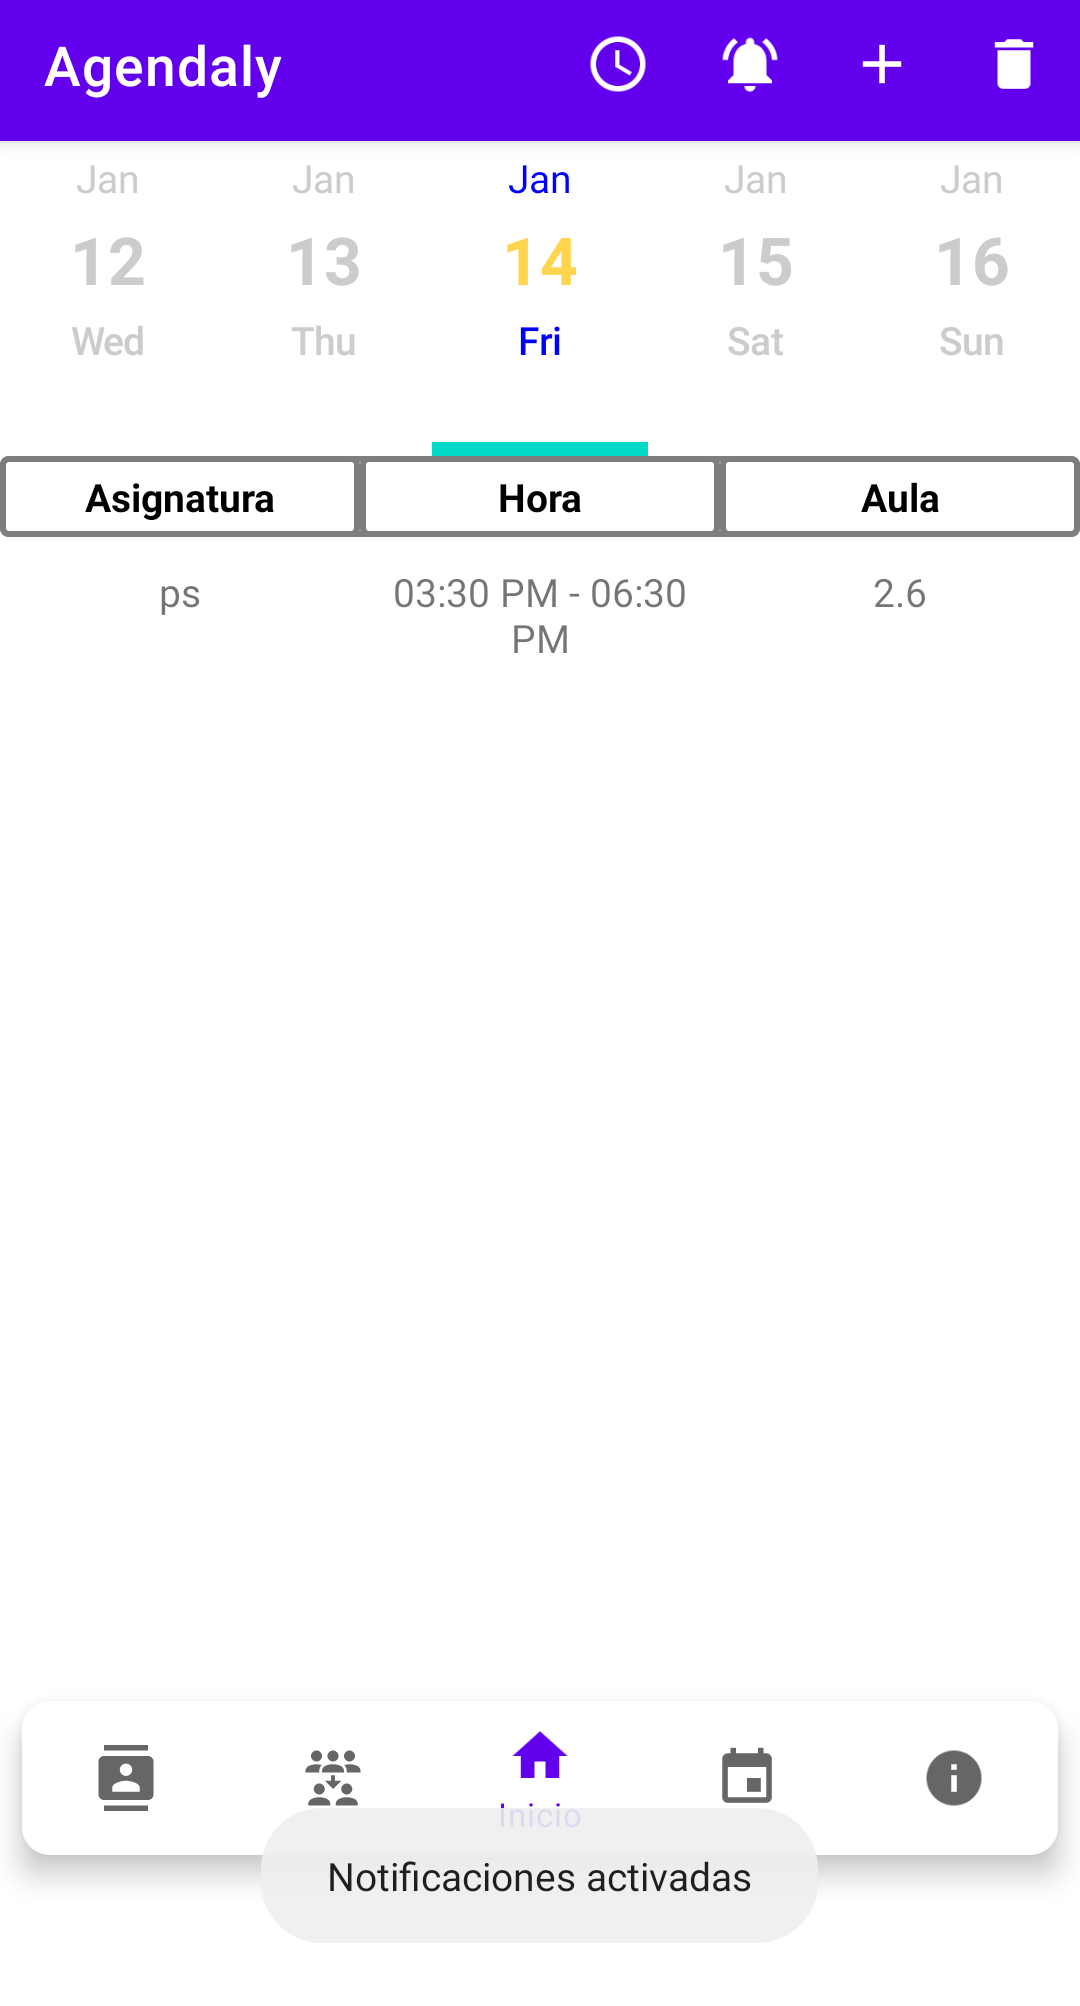
\includegraphics[scale=0.05]{notificacion2.png} 
        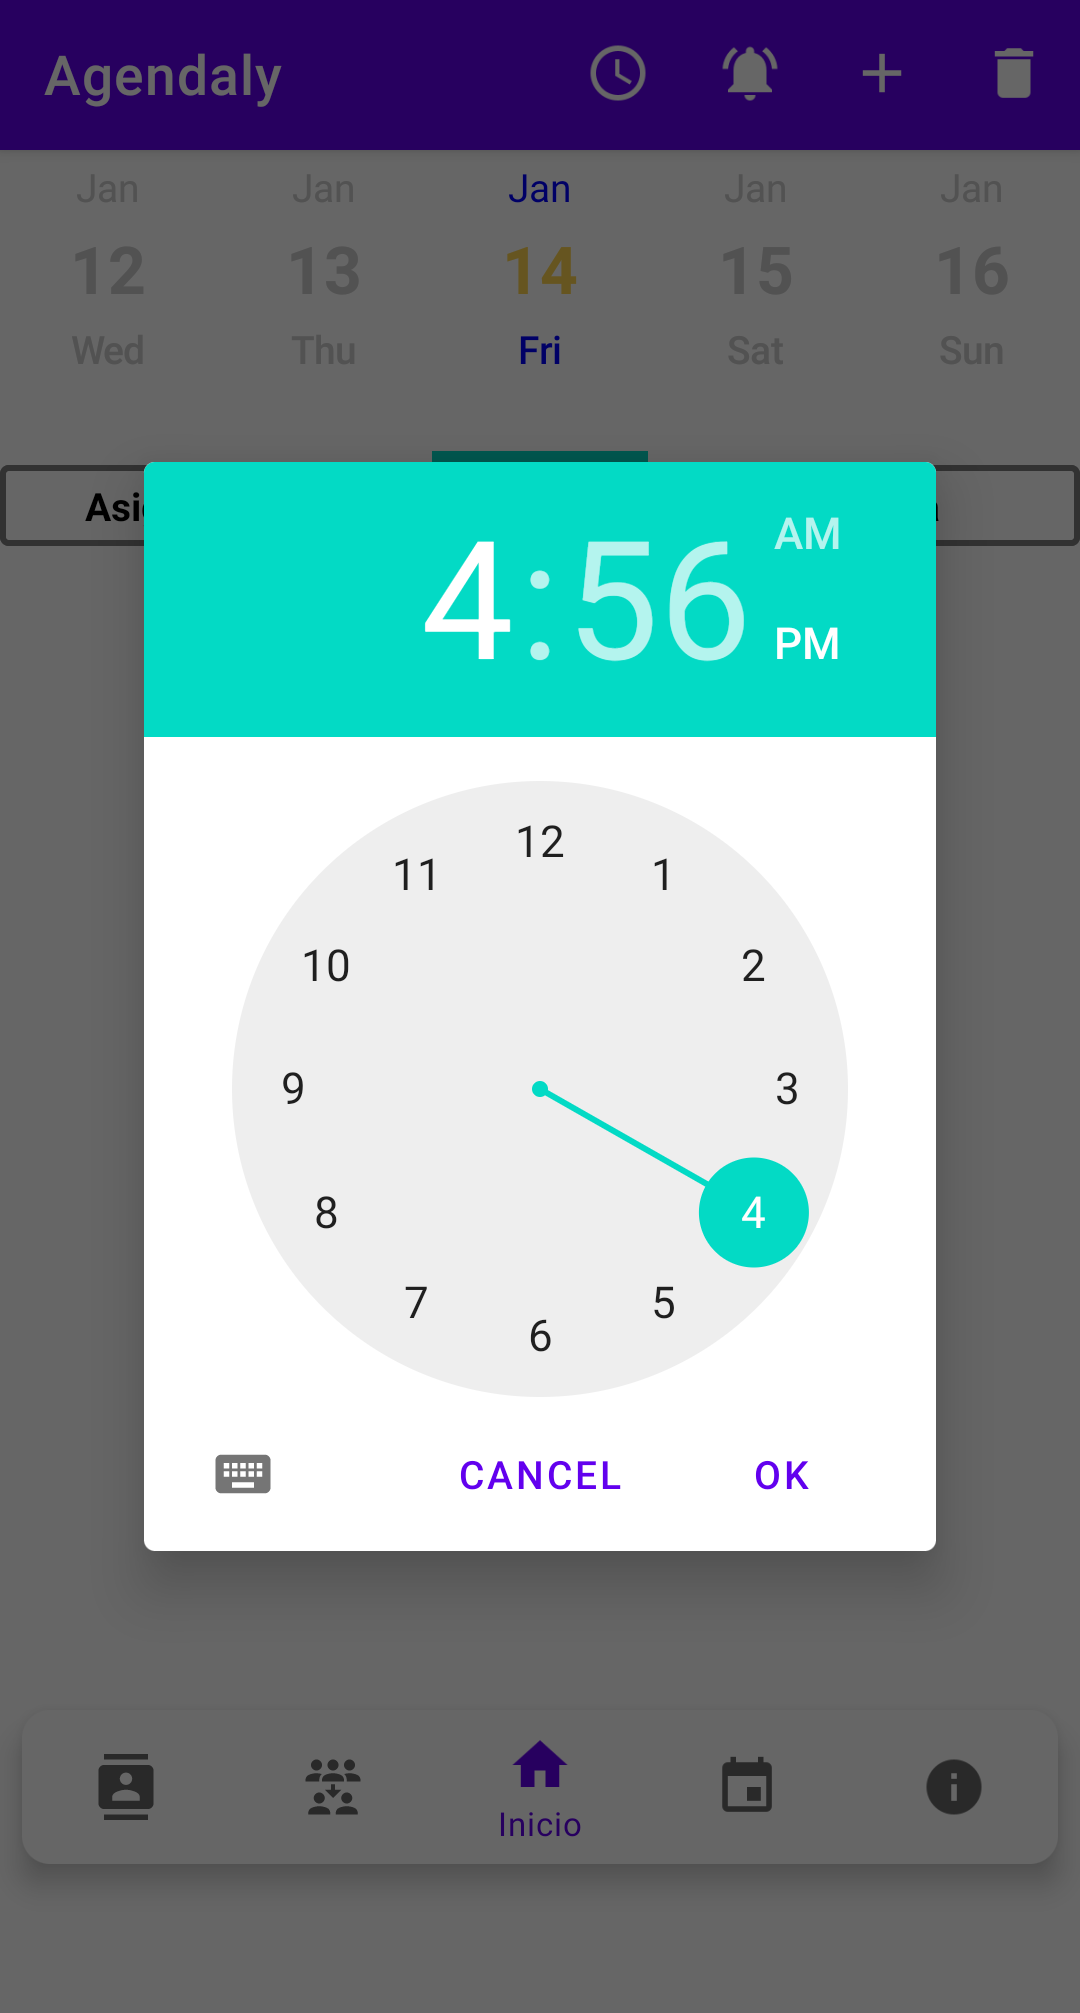
\includegraphics[scale=0.05]{notificacion3.png} 
        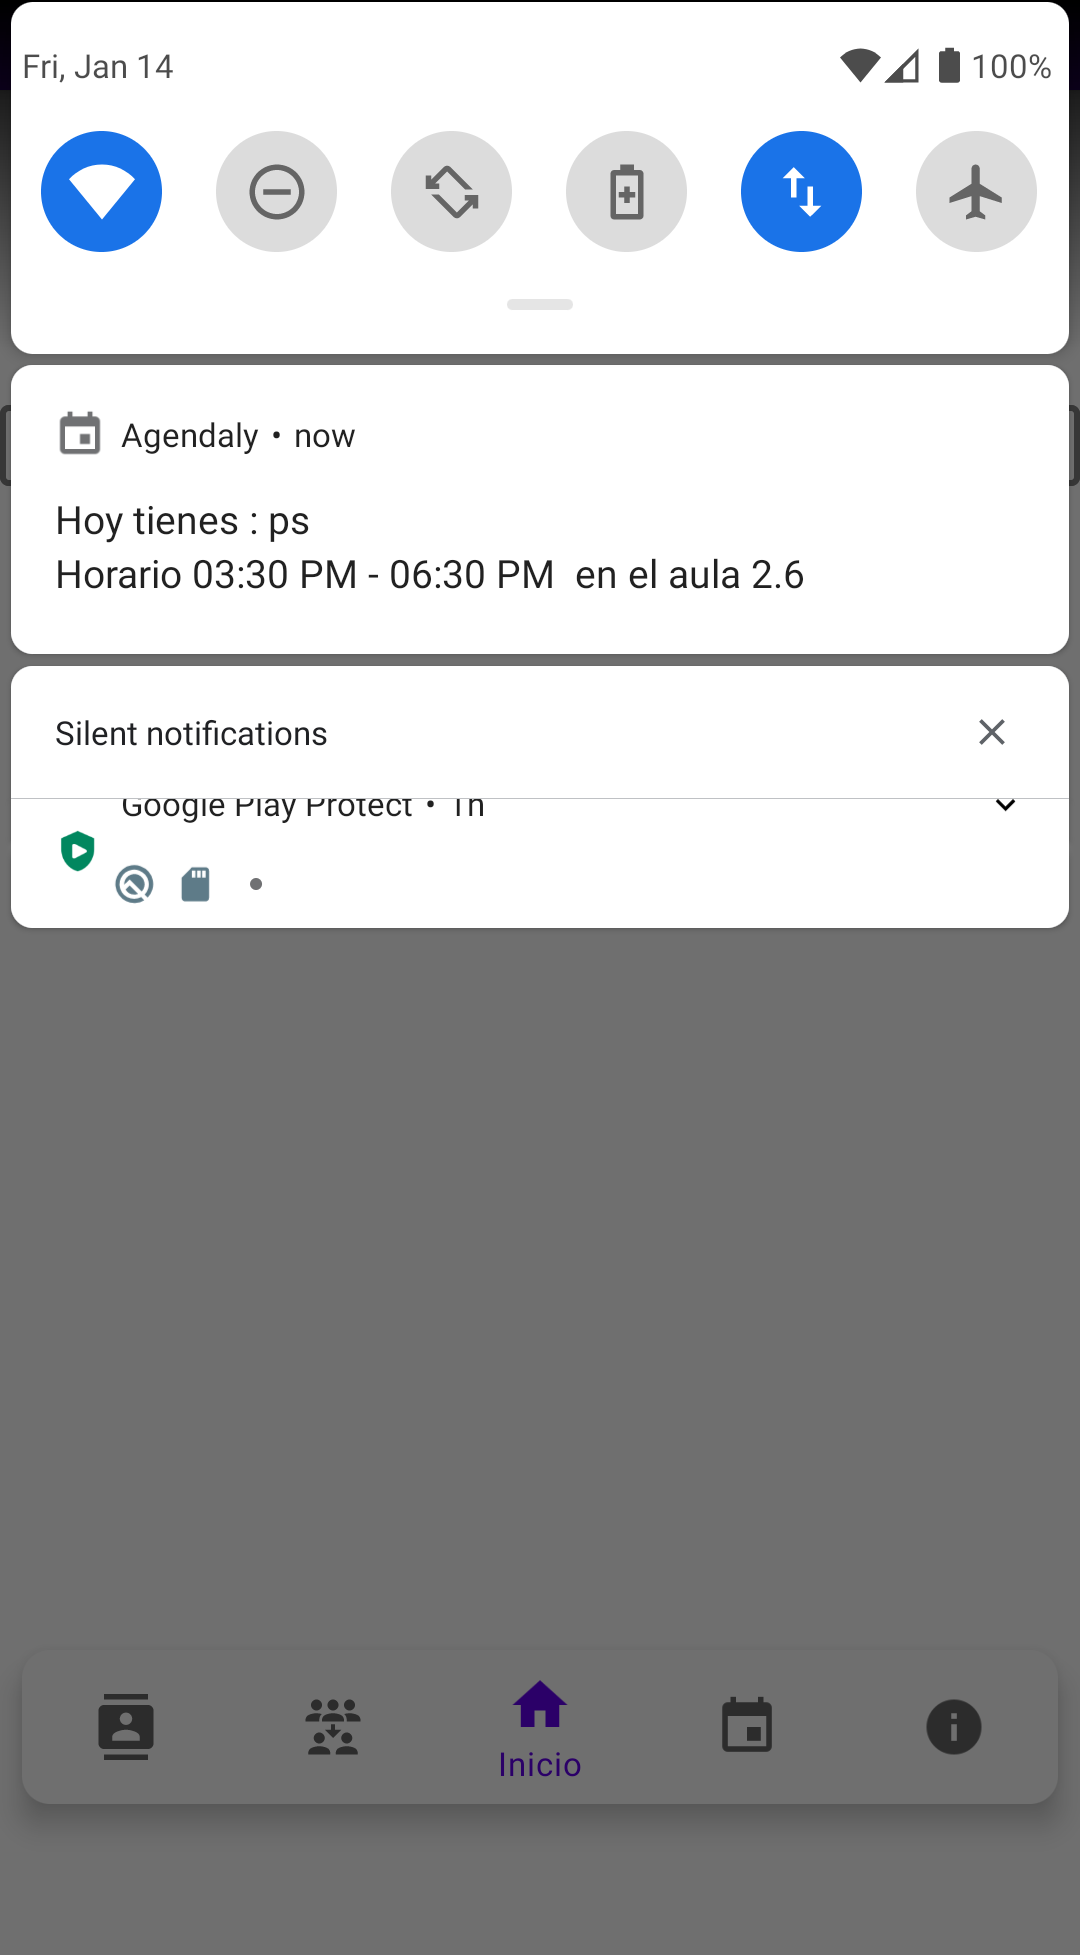
\includegraphics[scale=0.05]{notificacion8.png}
        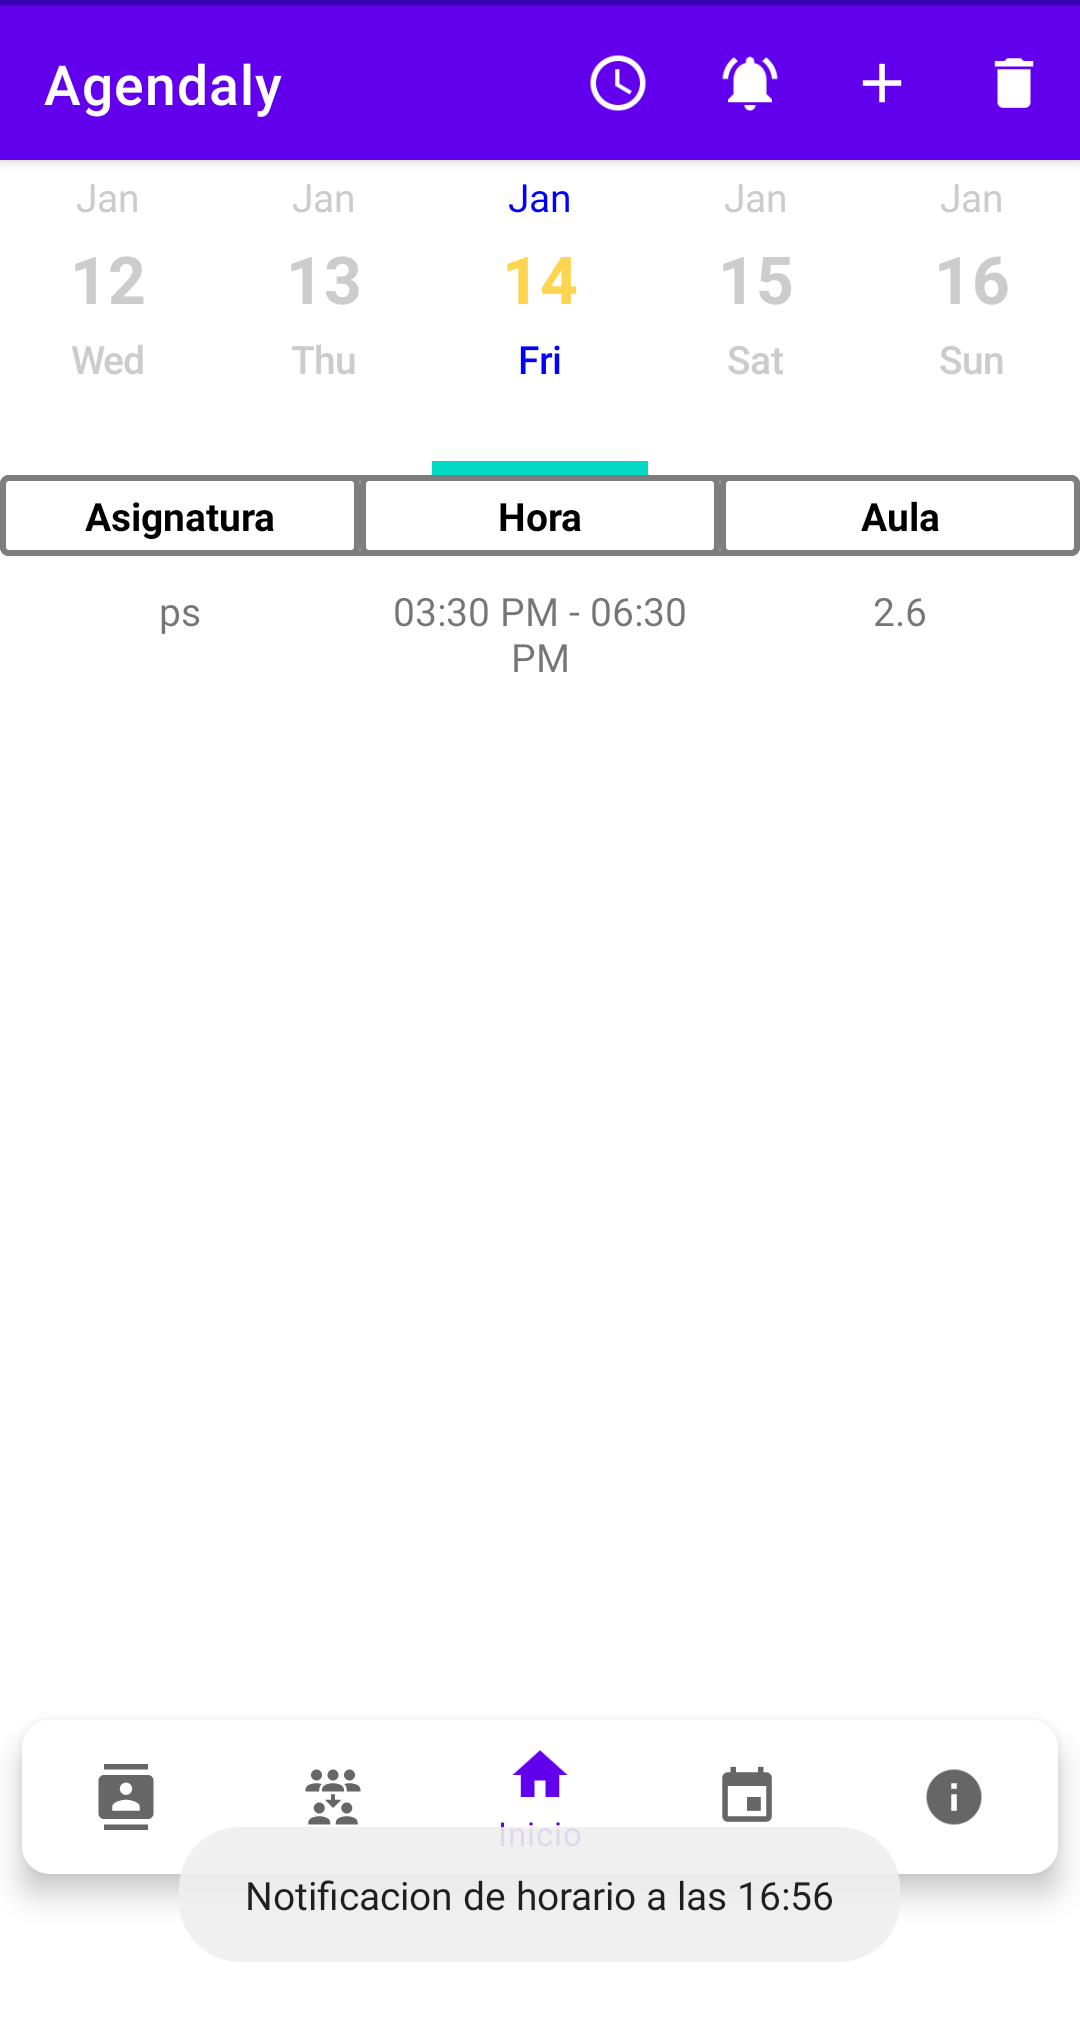
\includegraphics[scale=0.05]{notificacion4.png}\hfill 
        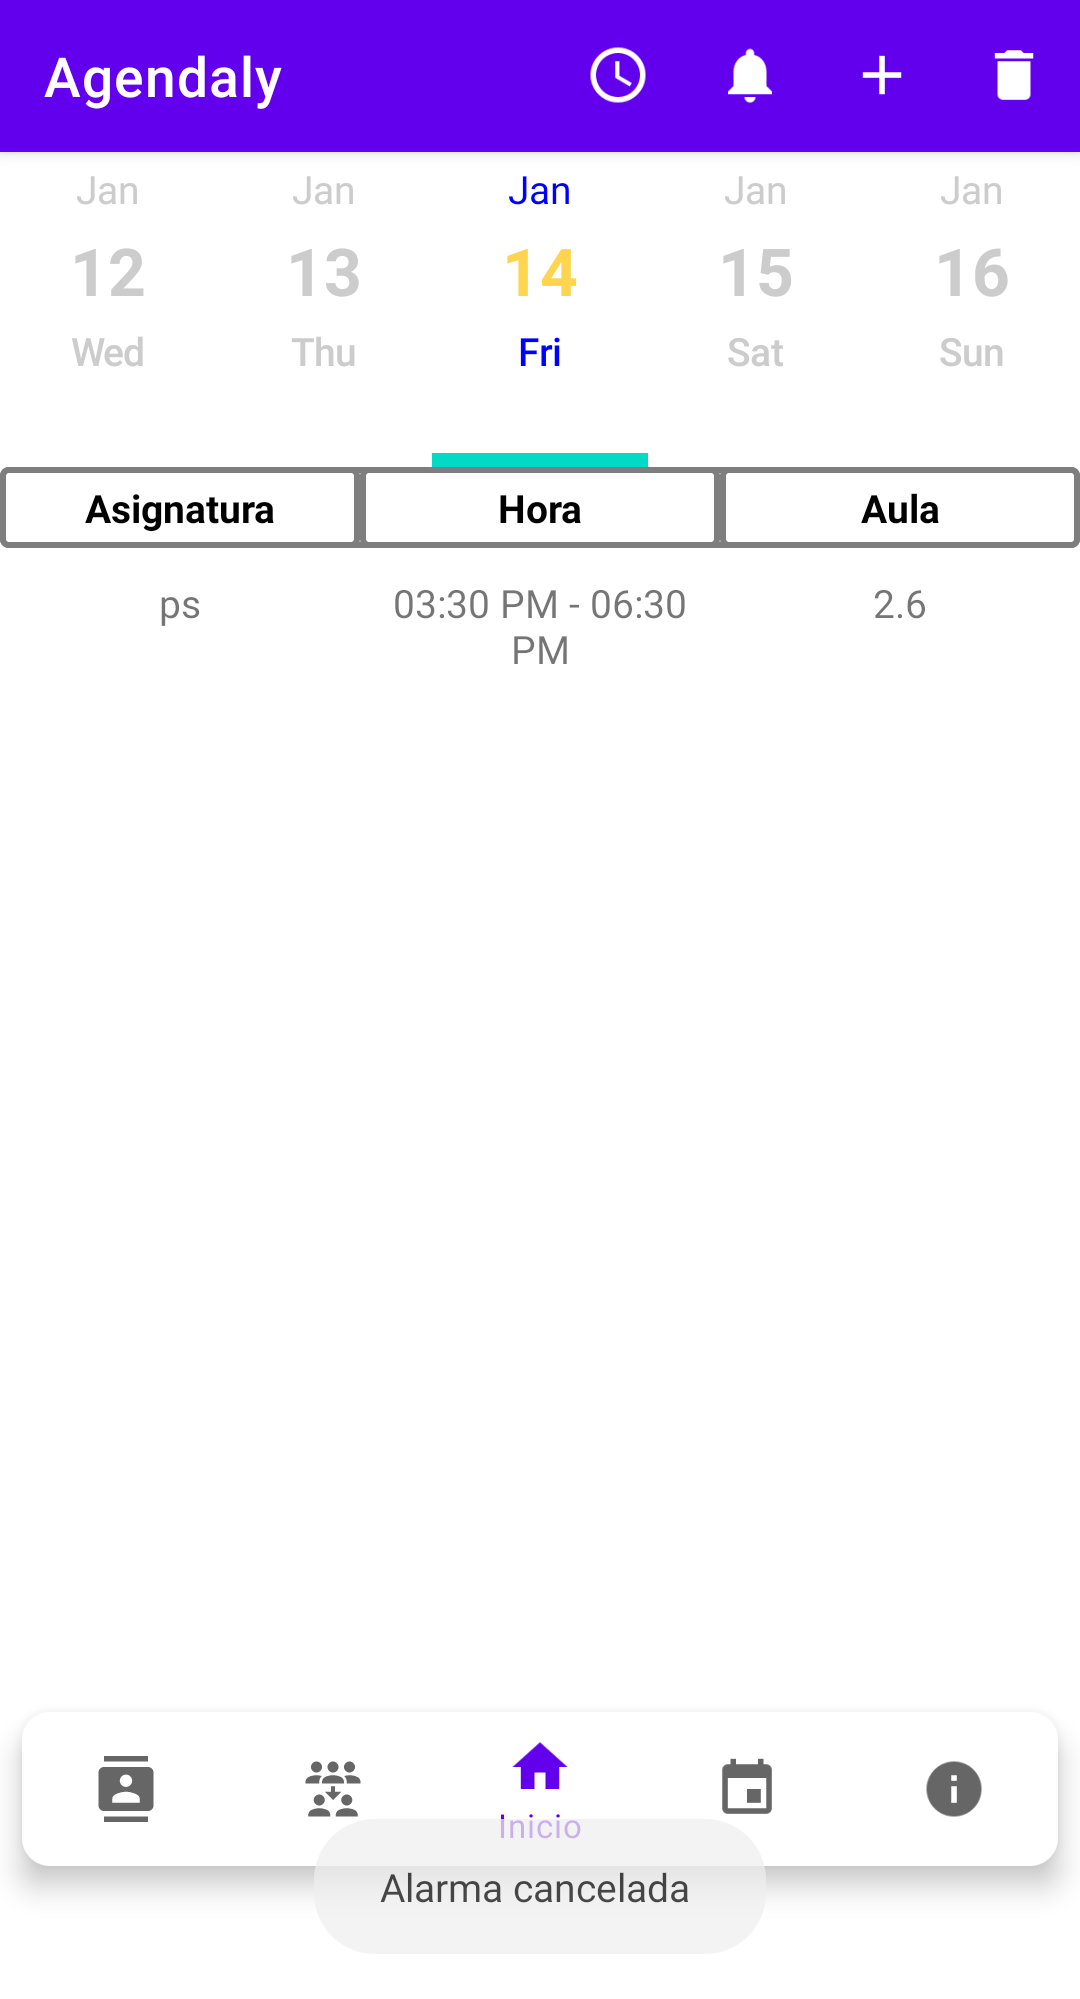
\includegraphics[scale=0.05]{notificacion5.png} 
        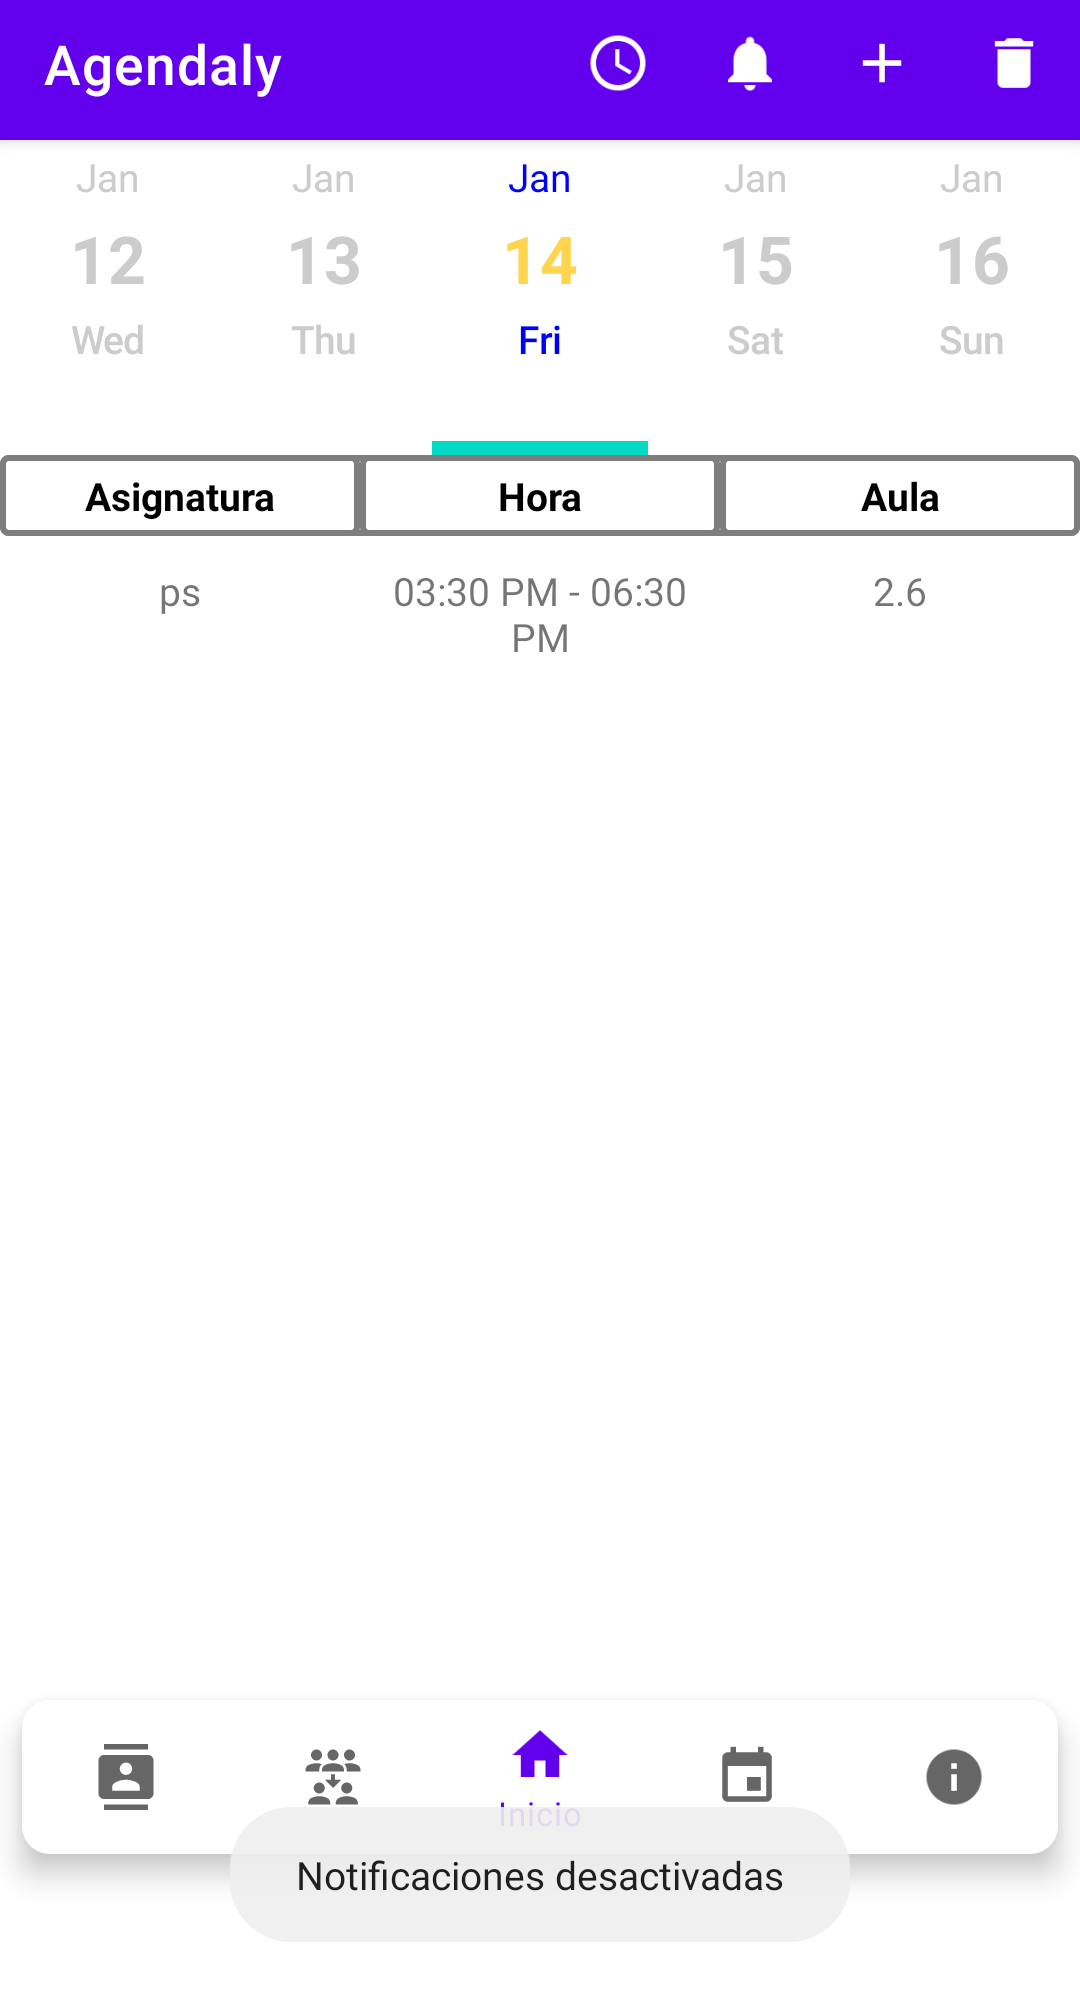
\includegraphics[scale=0.05]{notificacion6.png} 
        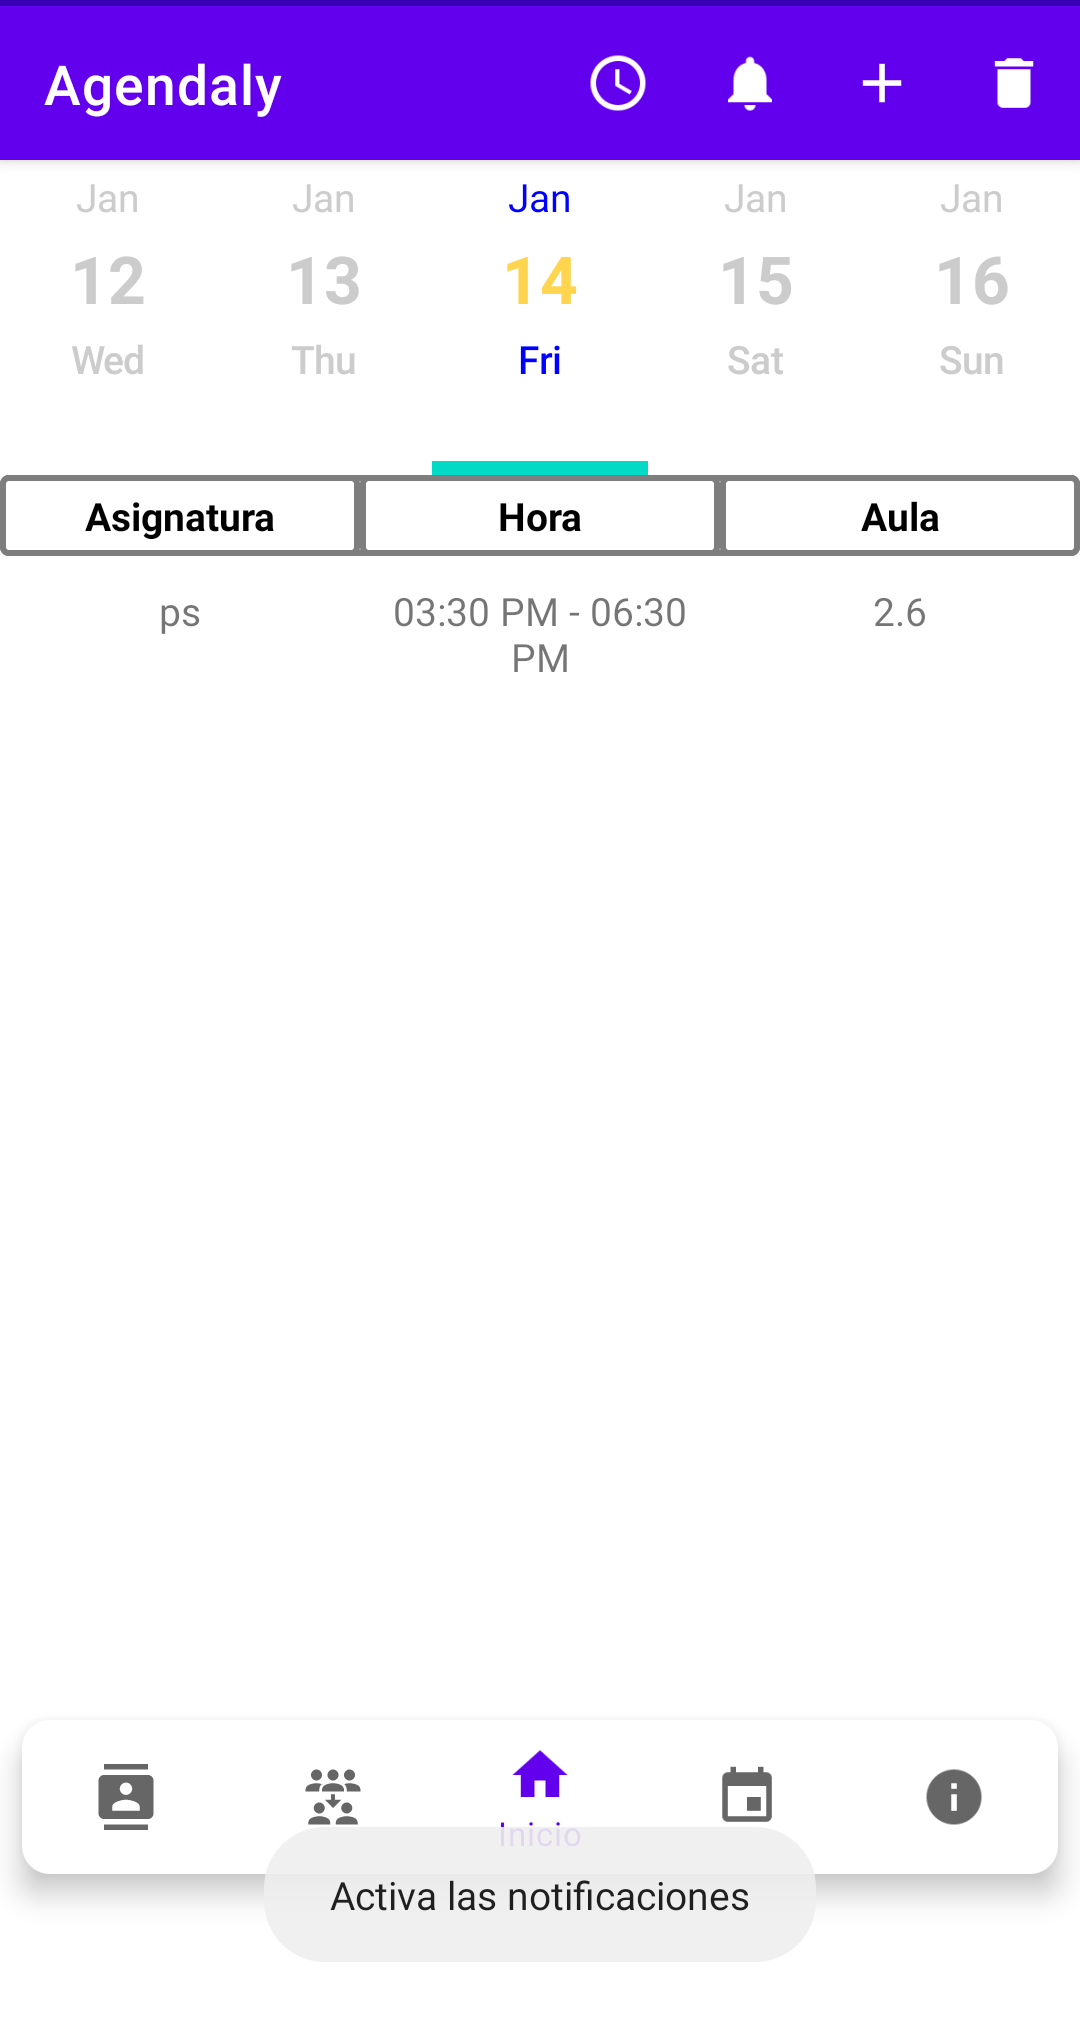
\includegraphics[scale=0.05]{notificacion7.png} 
            \caption{Pantallas de las notificaciones del horario}
        \end{figure}


\begin{figure}
            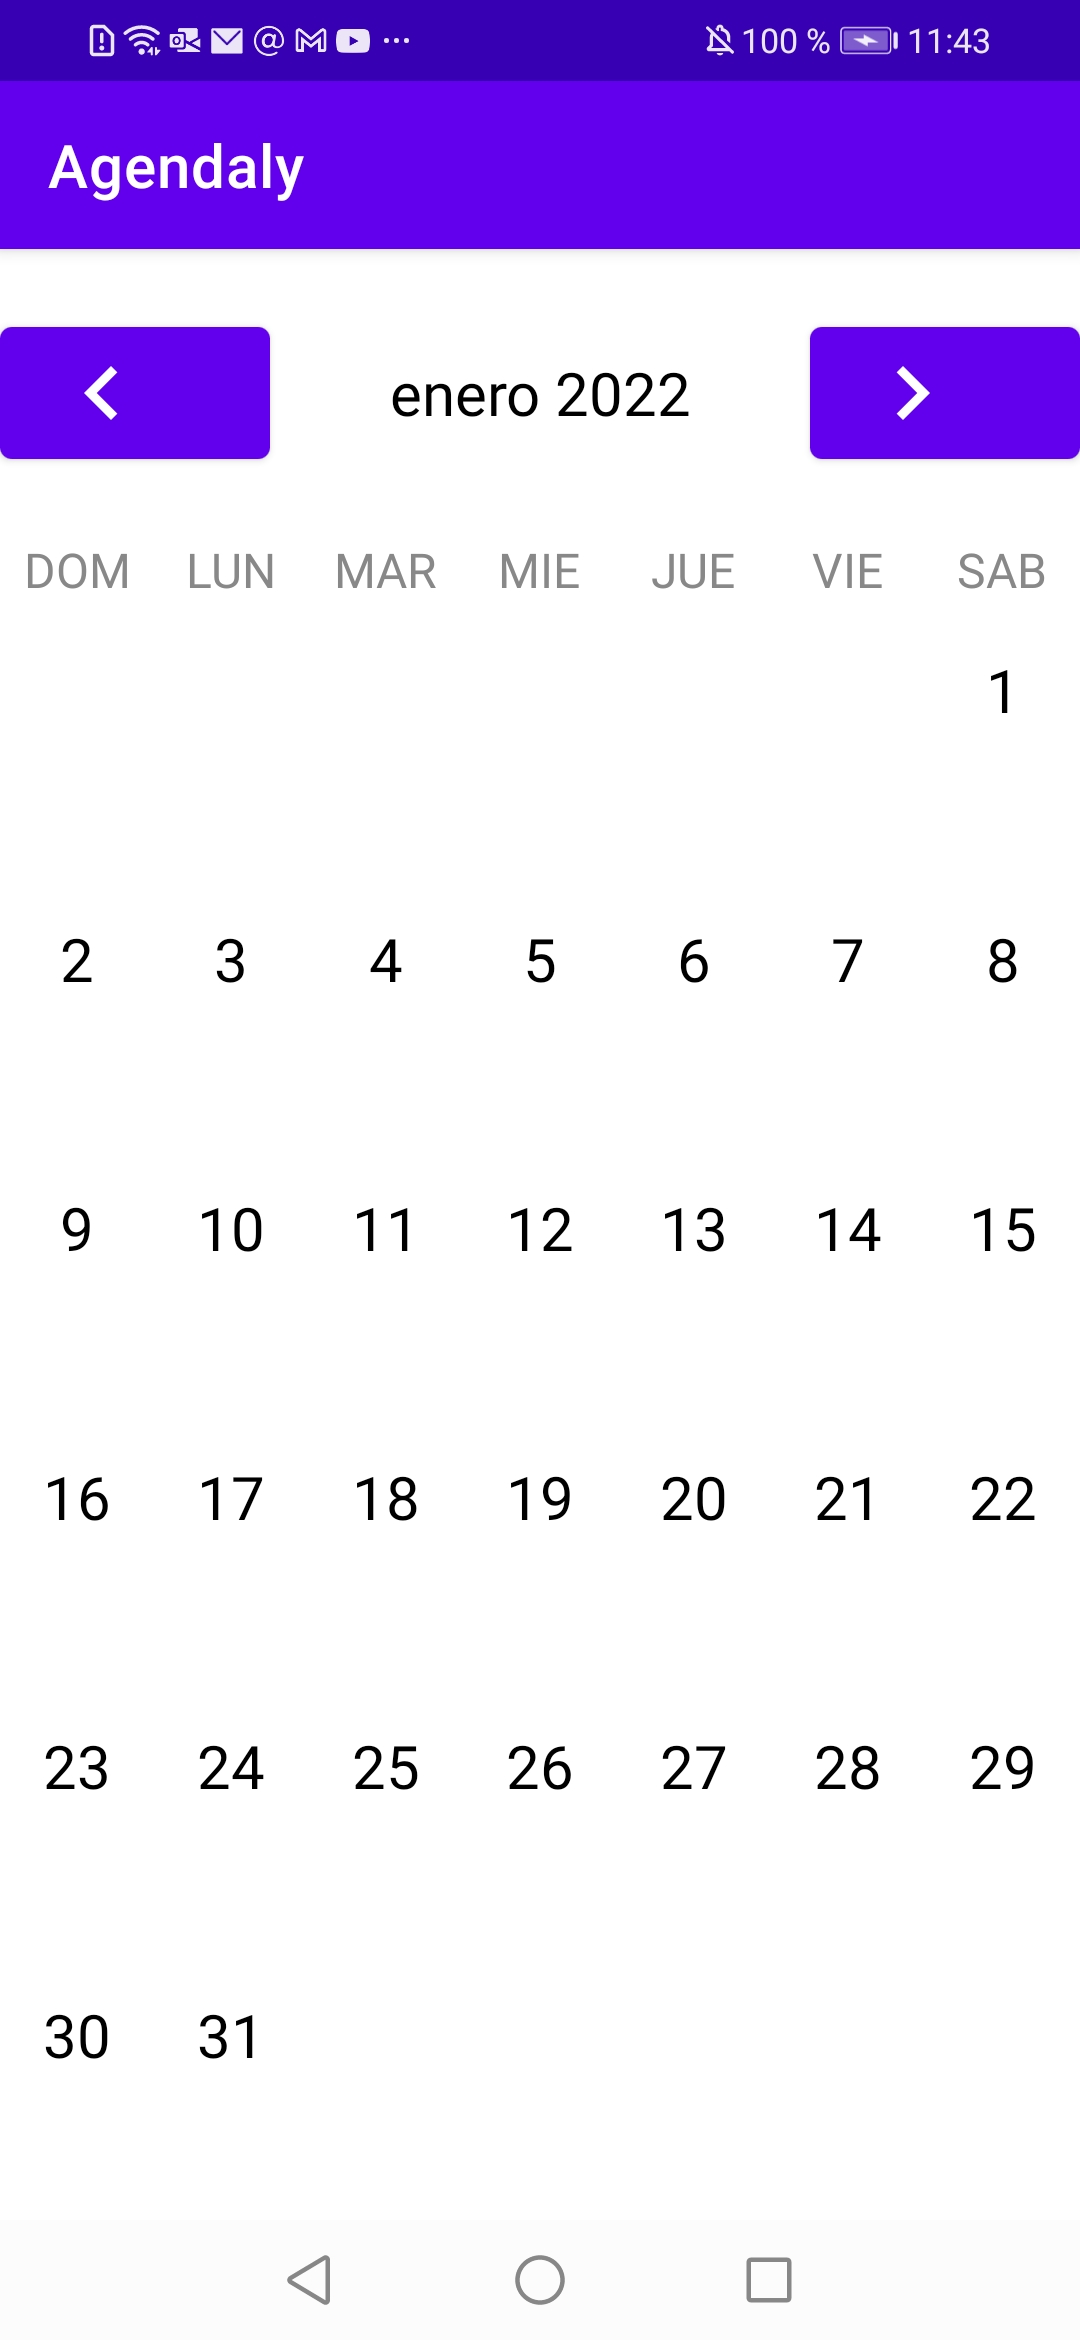
\includegraphics[scale=0.05]{calendar1.jpg} \hfill
            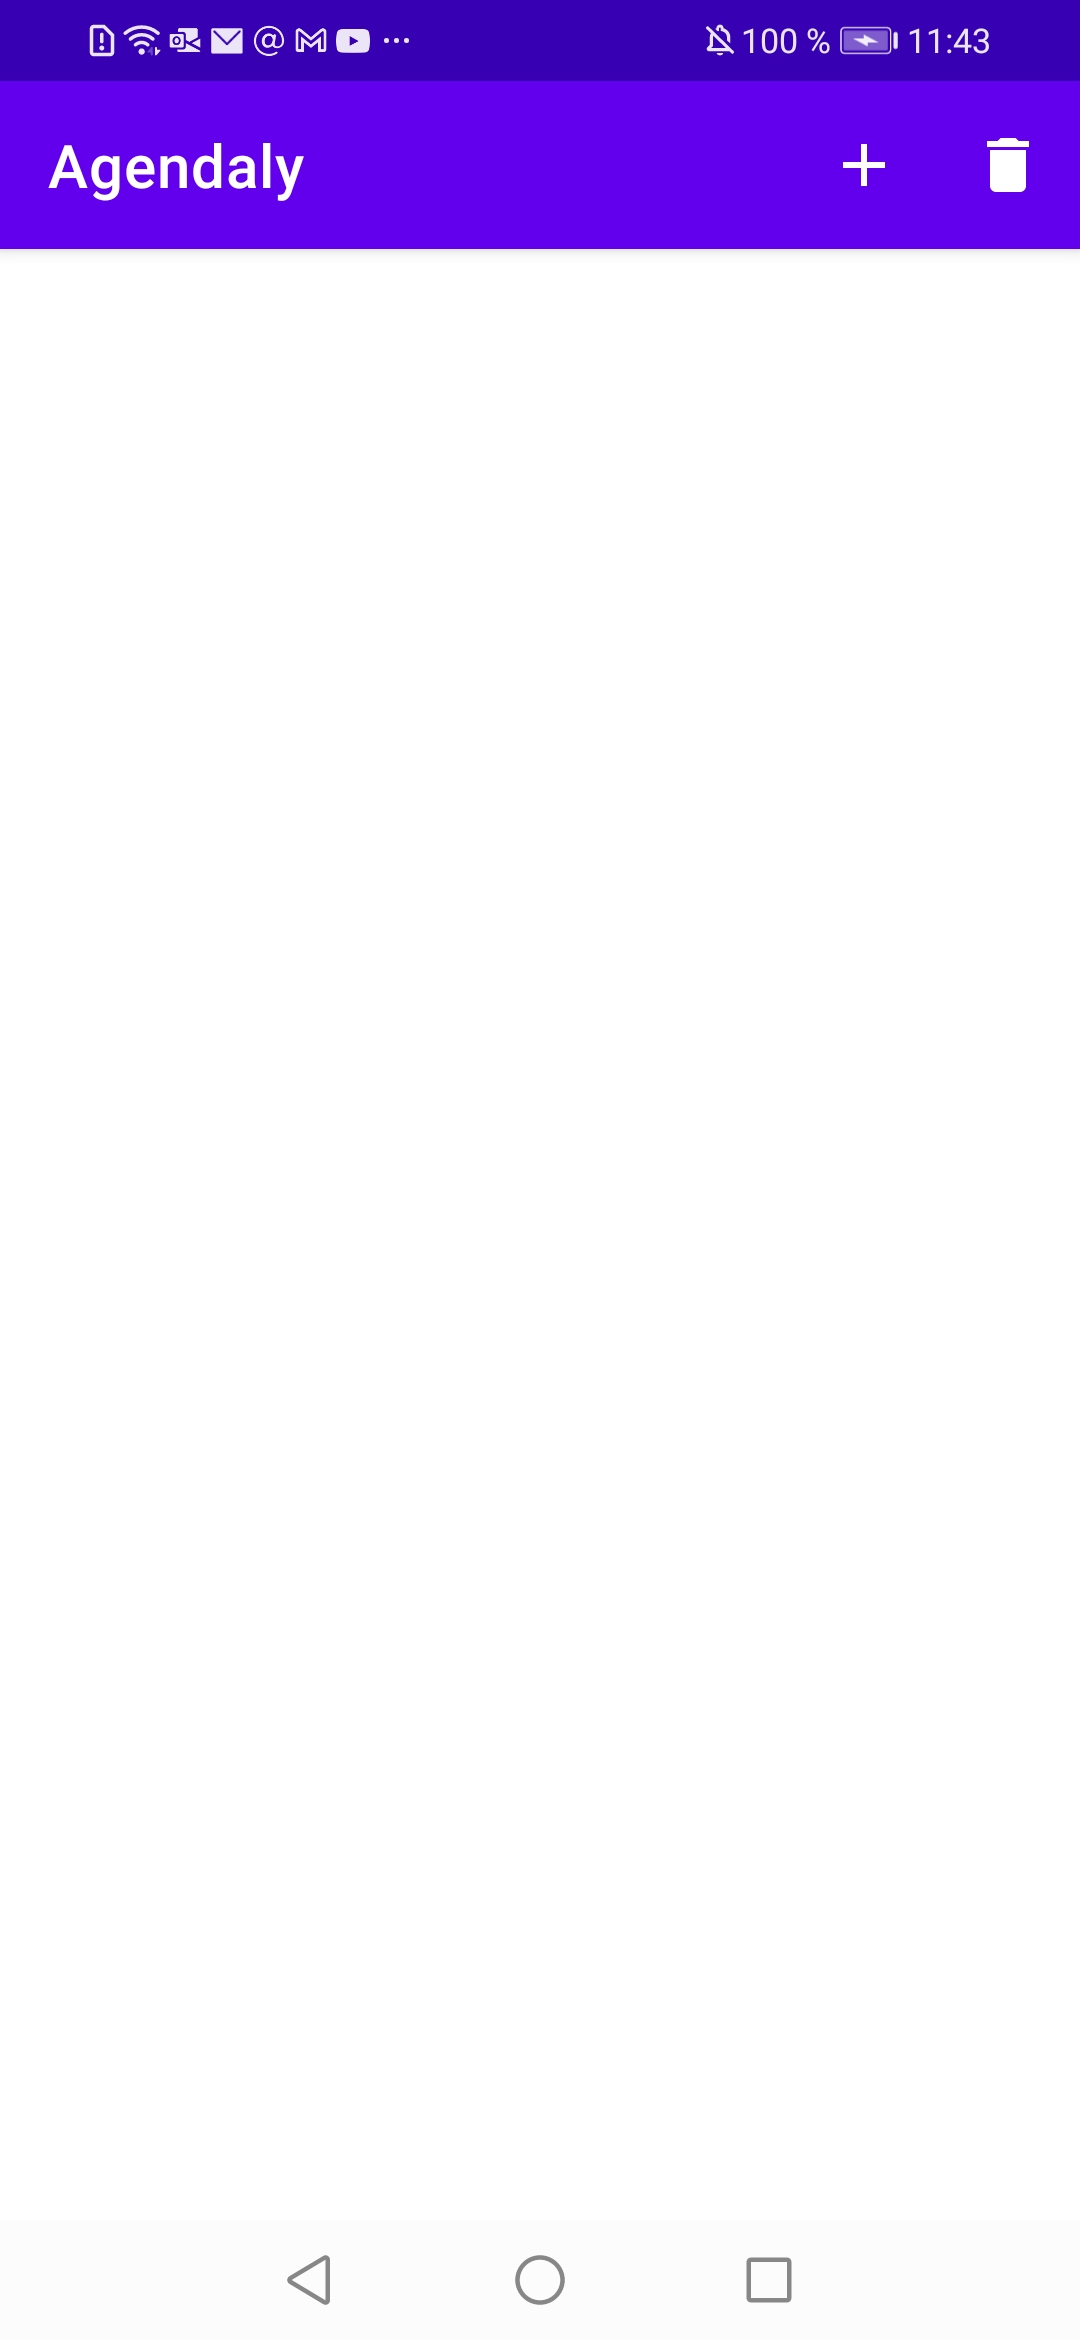
\includegraphics[scale=0.05]{calendar2.jpg}\hfill
            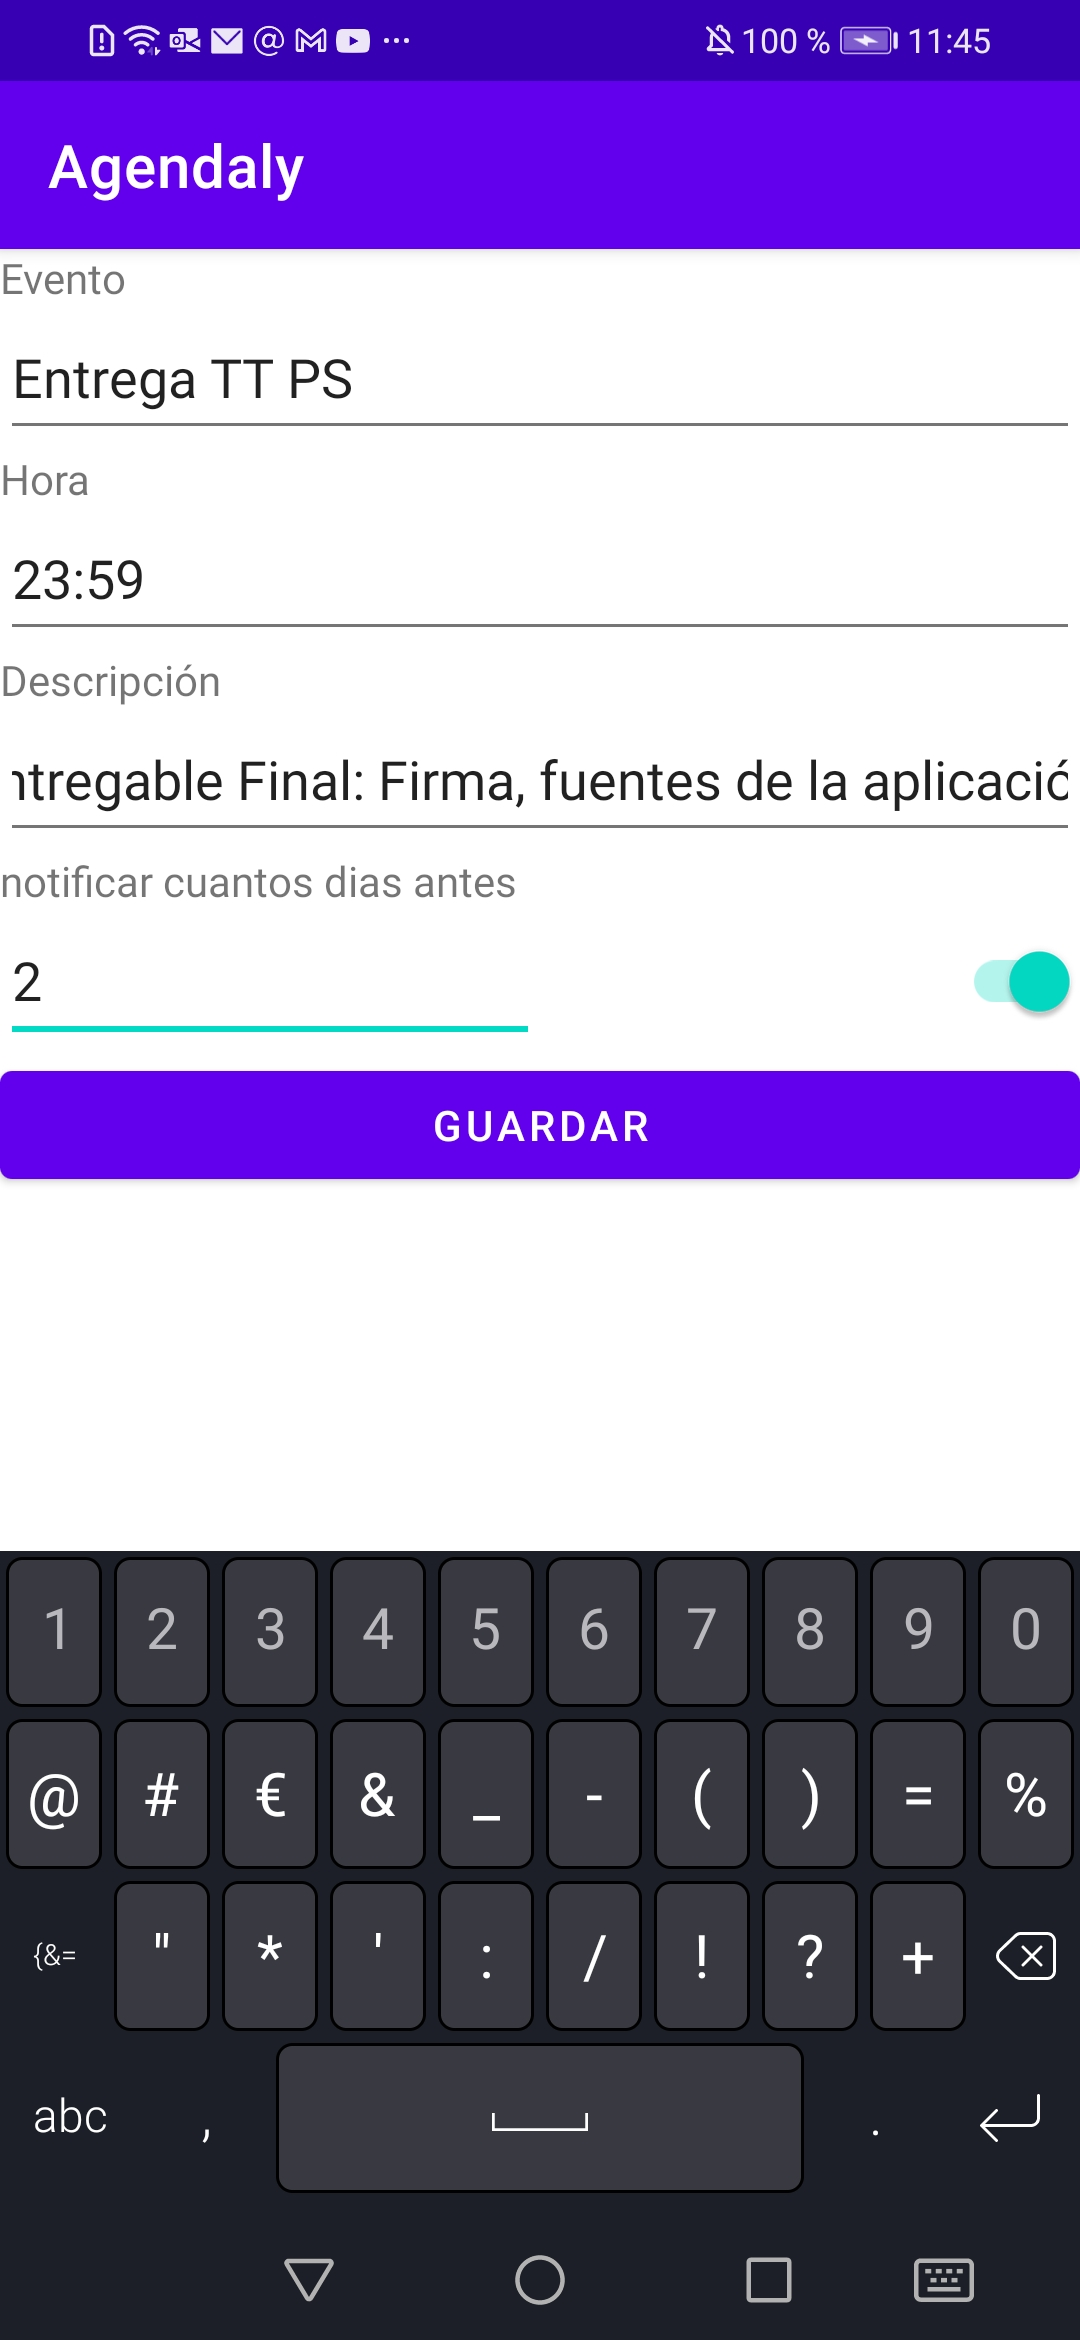
\includegraphics[scale=0.05]{calendar3.jpg} \hfill
            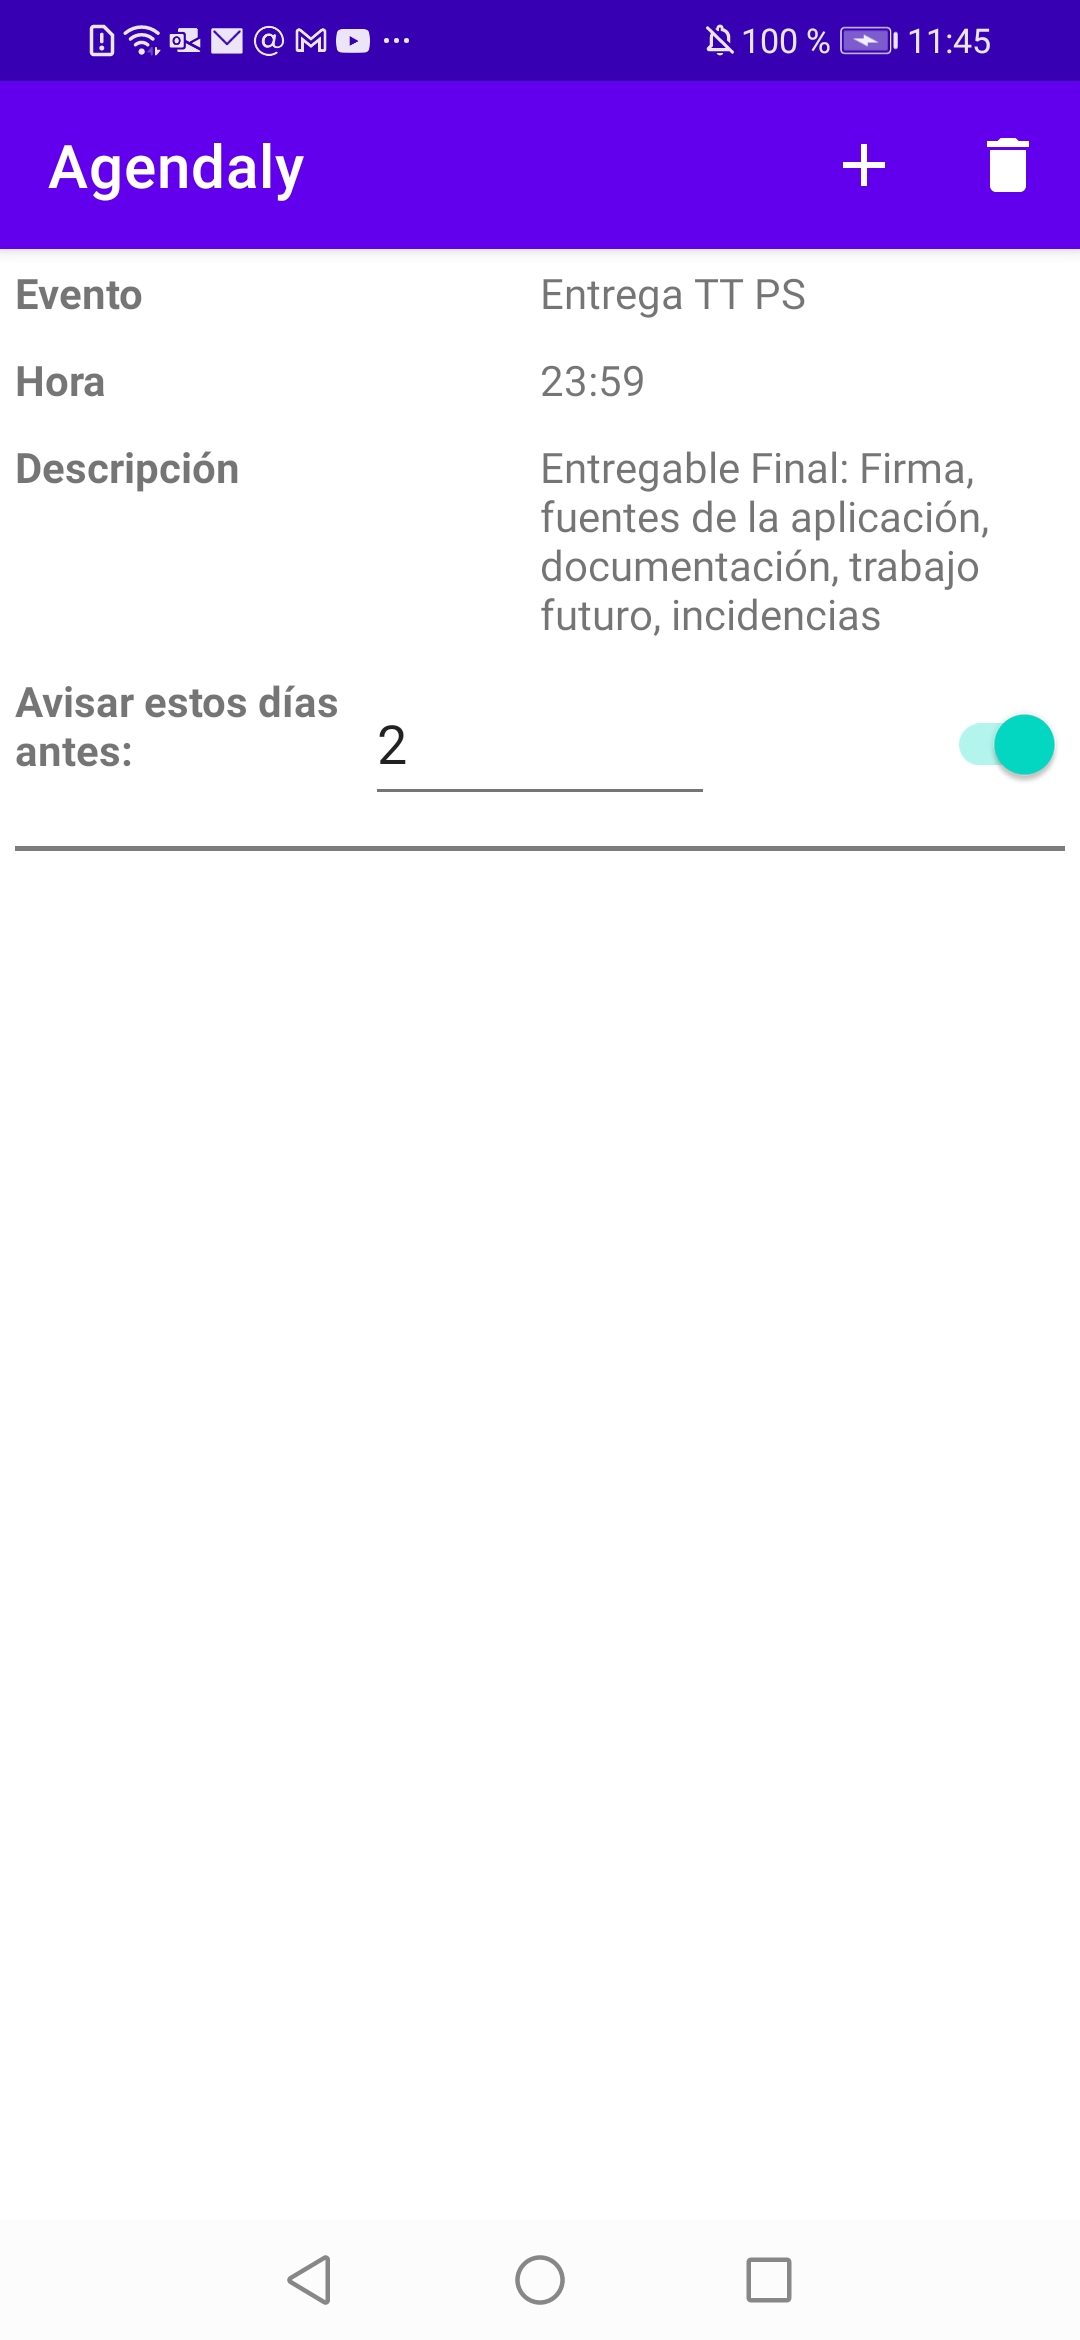
\includegraphics[scale=0.05]{calendar4.jpg}\hfill
            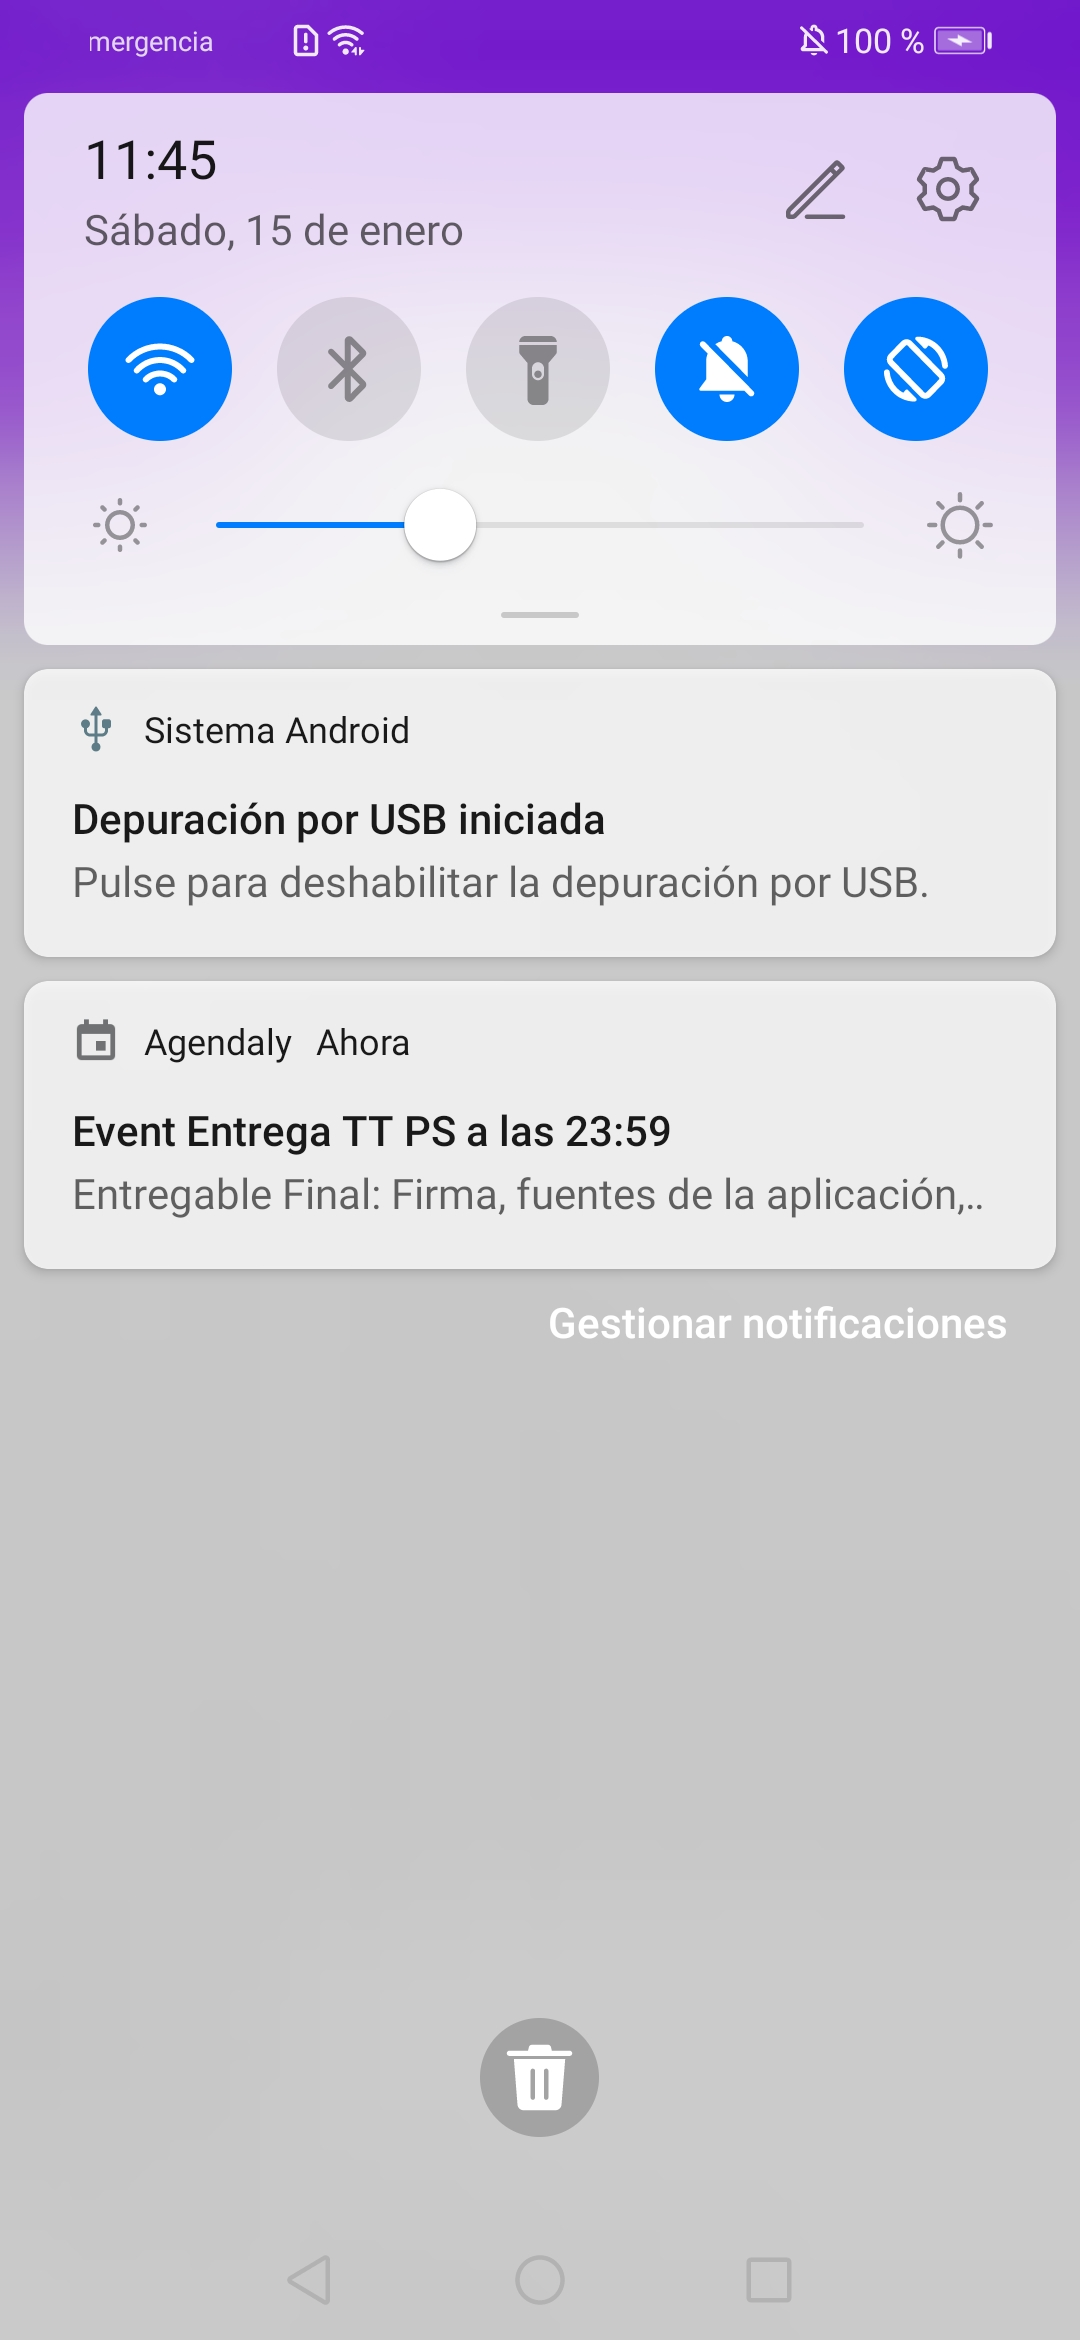
\includegraphics[scale=0.05]{calendar5.jpg}\hfill
            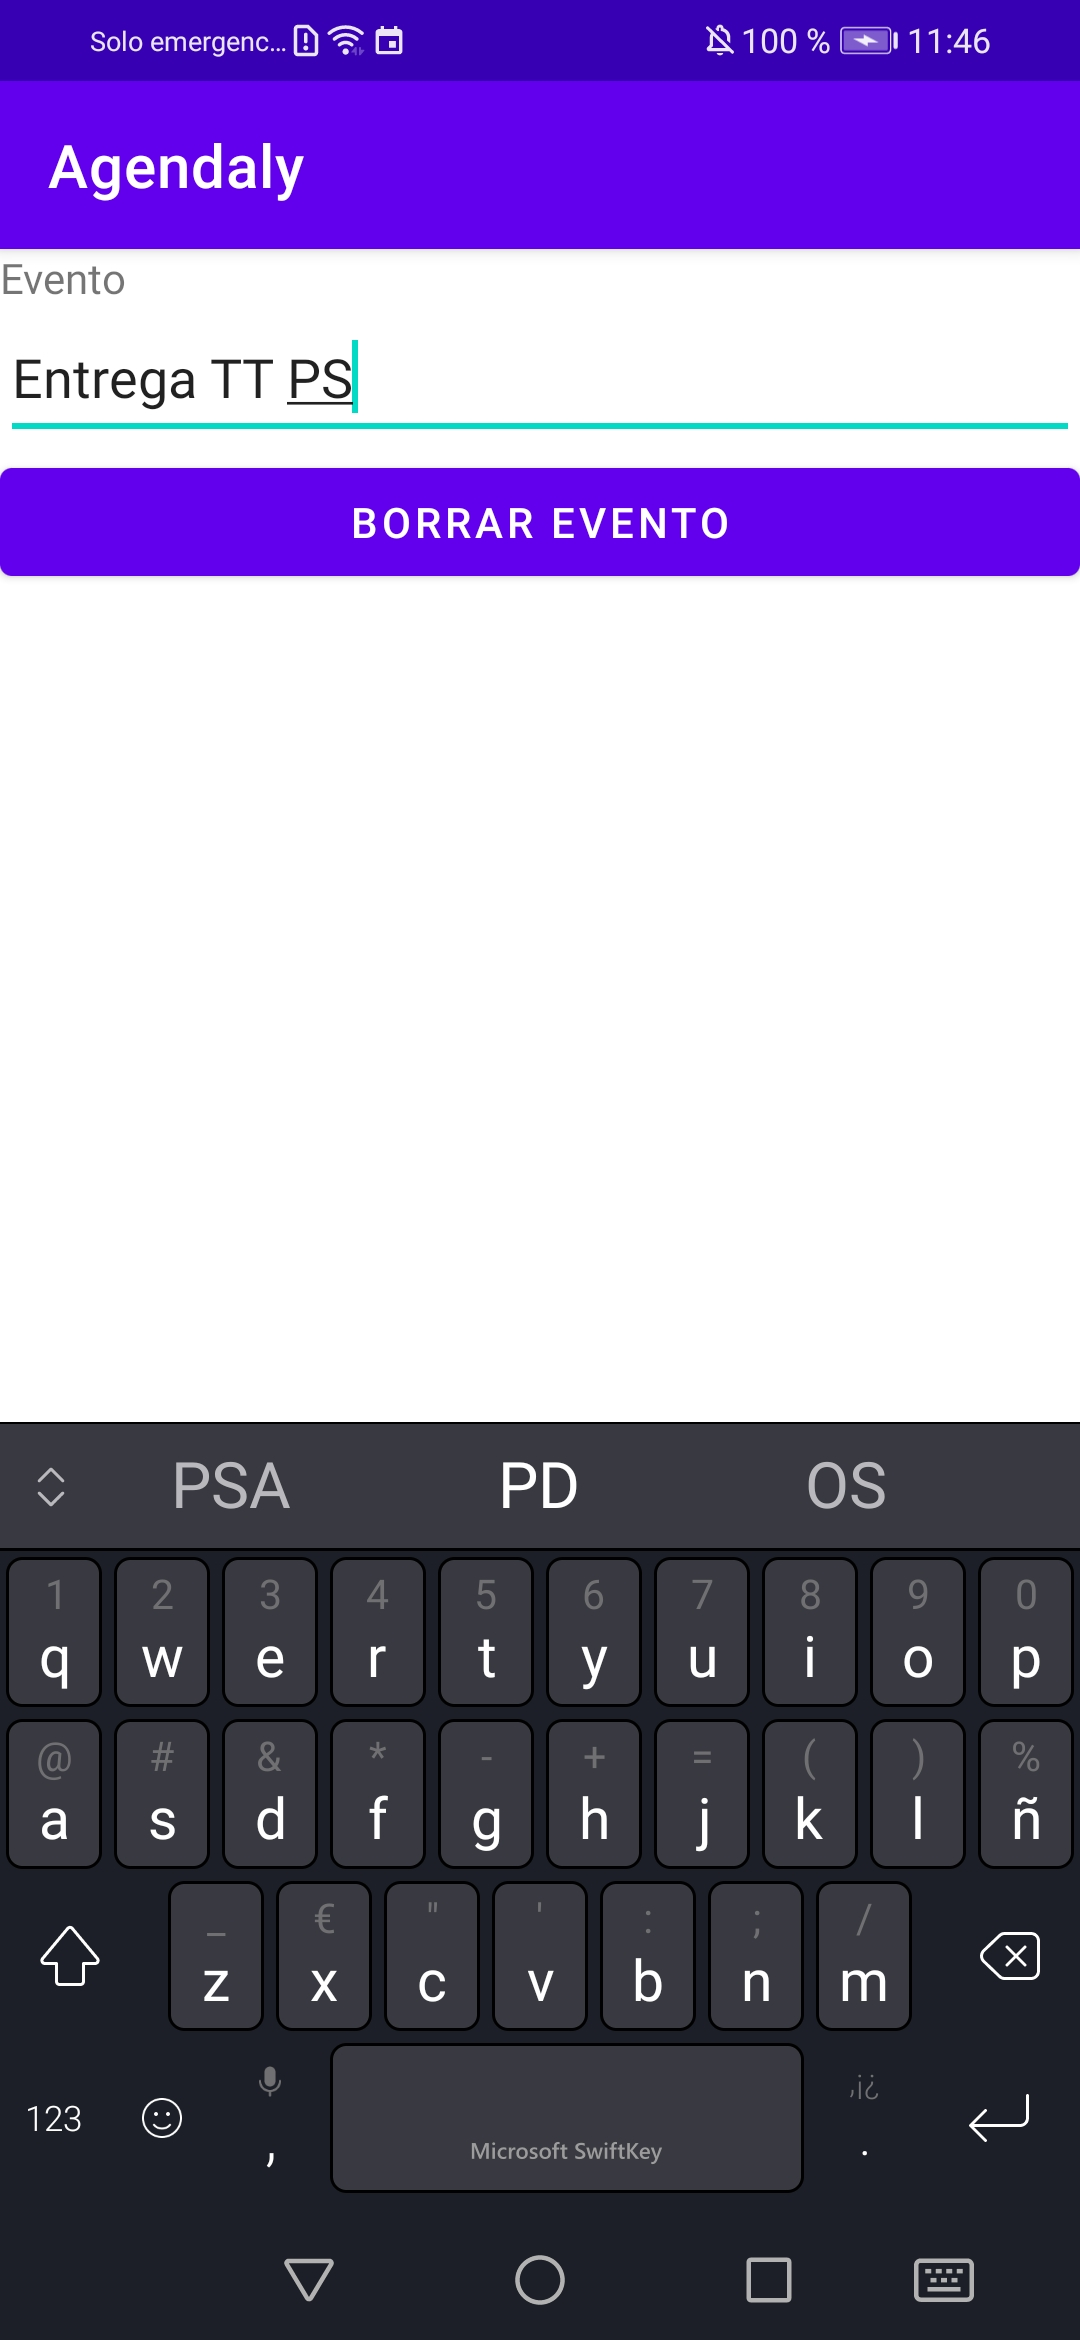
\includegraphics[scale=0.05]{calendar6.jpg}\hfill
            \caption{Pantallas del calendario y sus notificaciones}
        \end{figure}

\begin{figure}
    \centering
    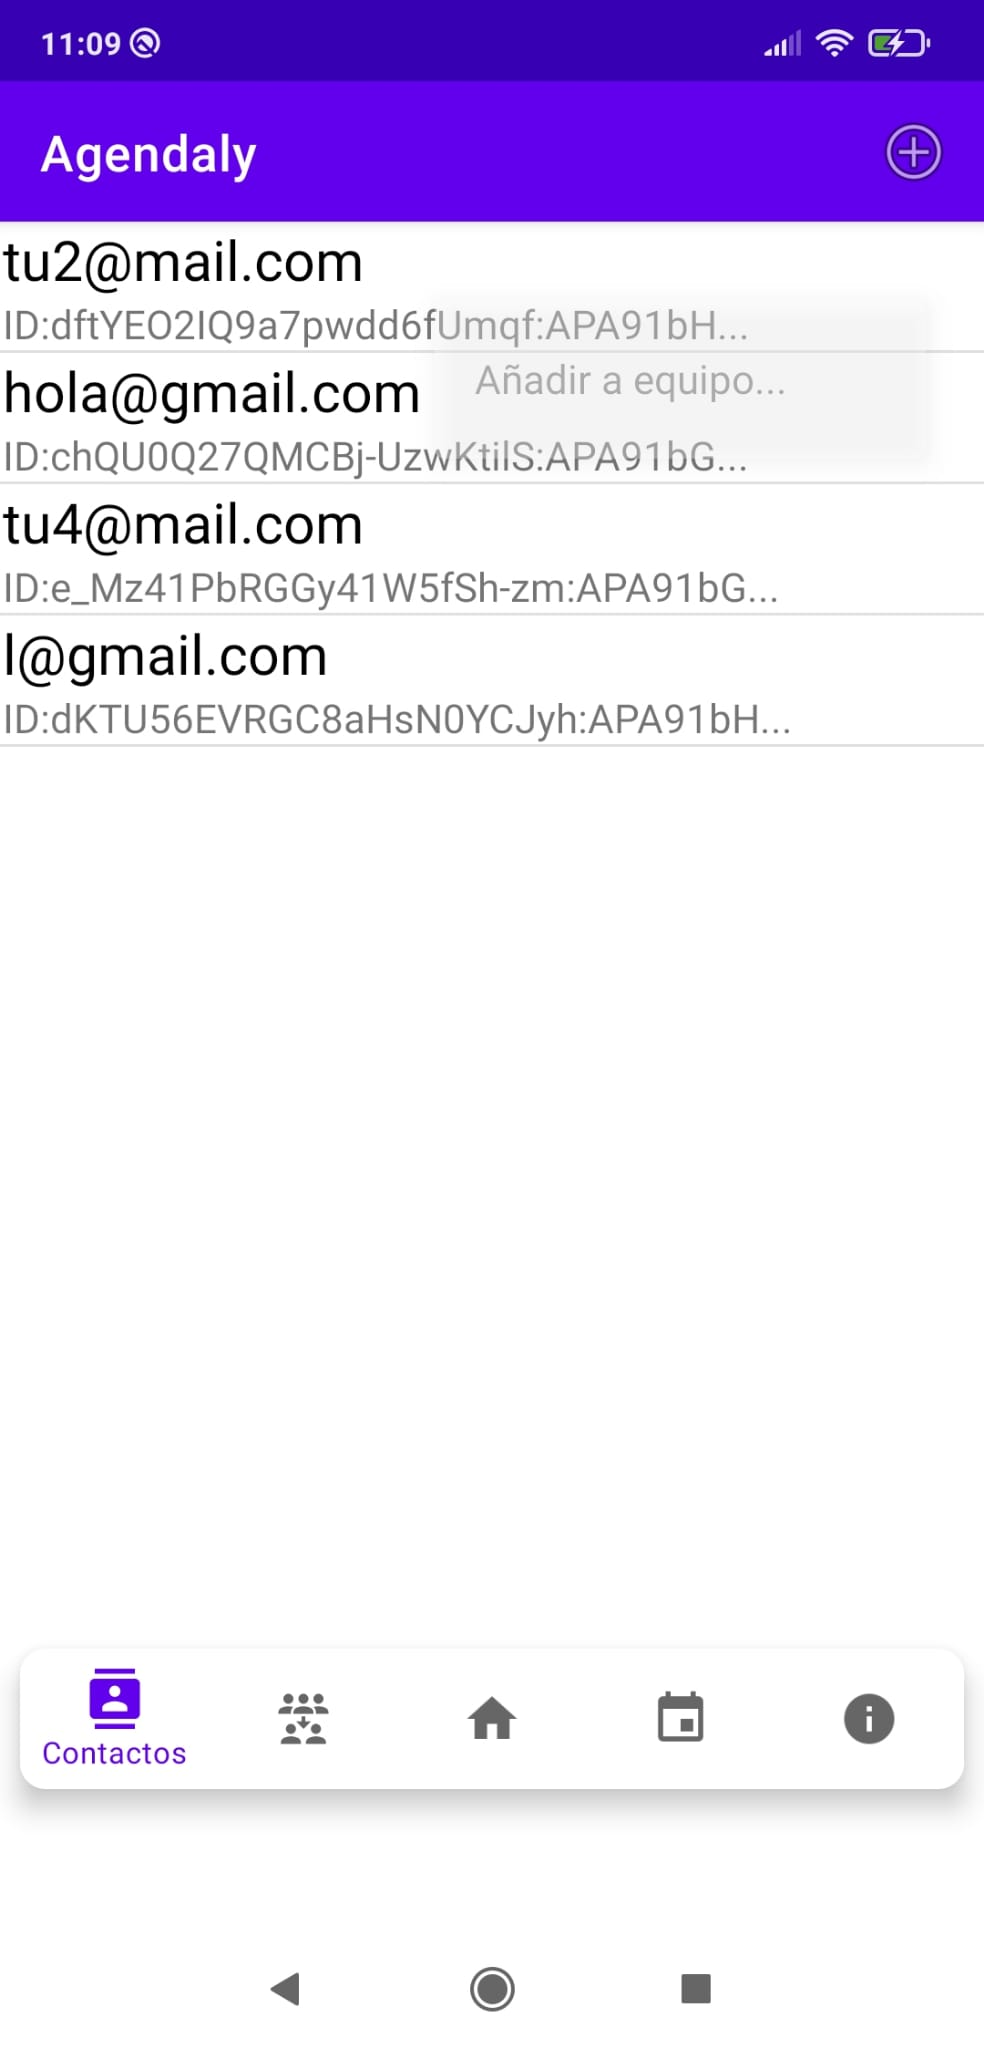
\includegraphics[scale=0.05]{contacts_view.jpeg} \hfill
    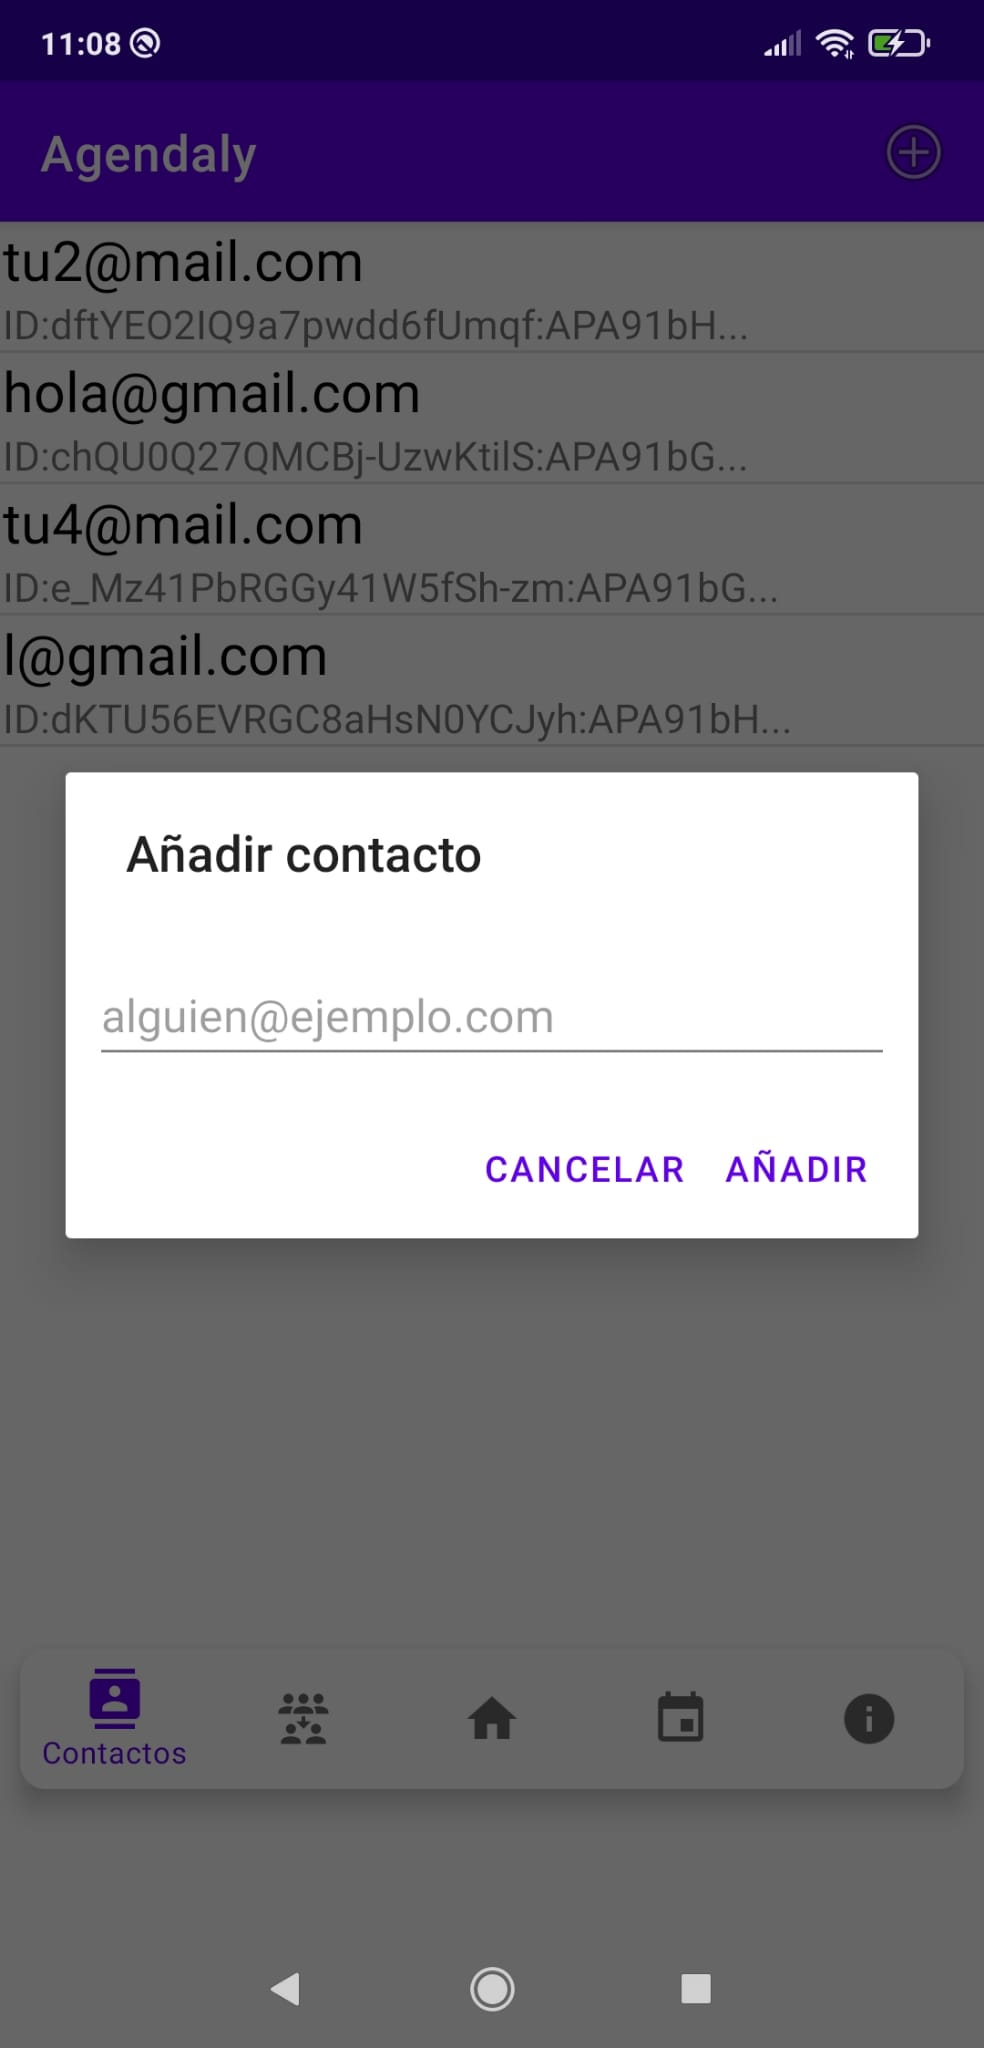
\includegraphics[scale=0.05]{add_contact.jpeg}\hfill
    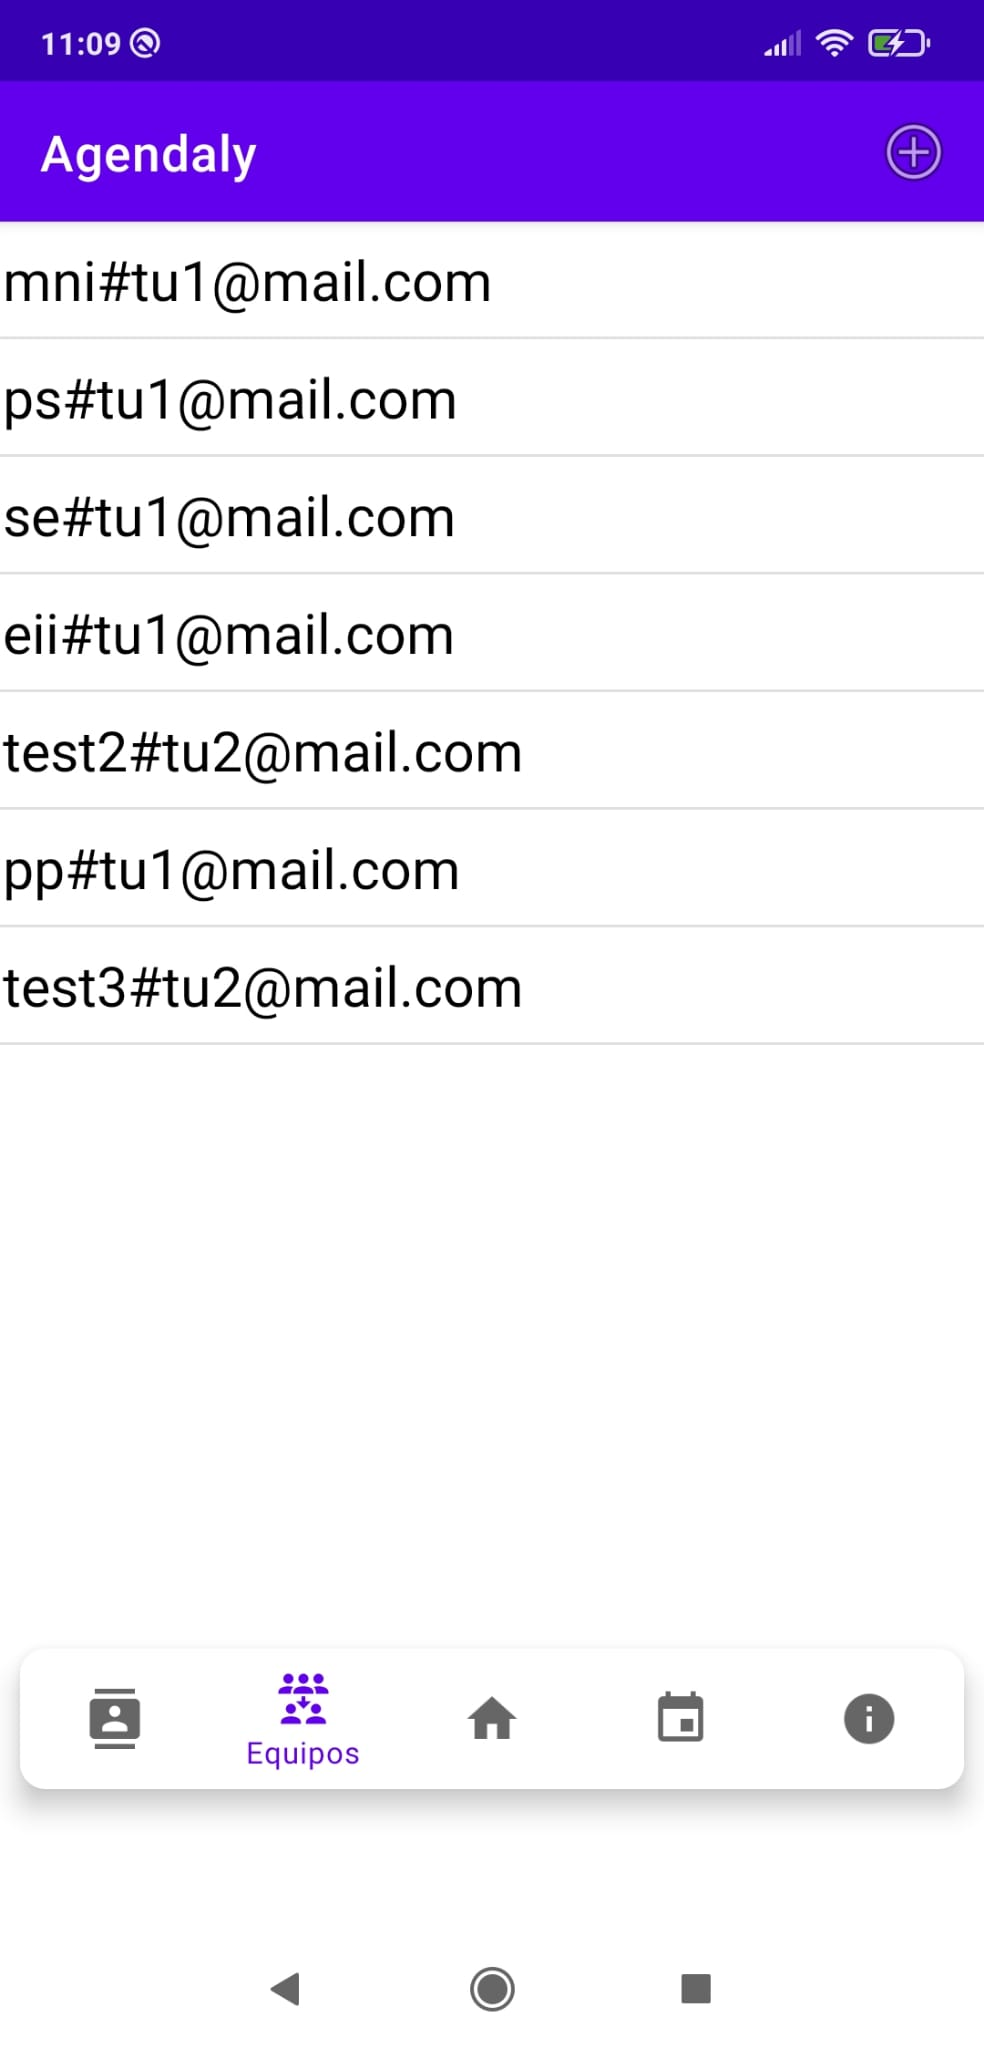
\includegraphics[scale=0.05]{teams_view.jpeg}\hfill
    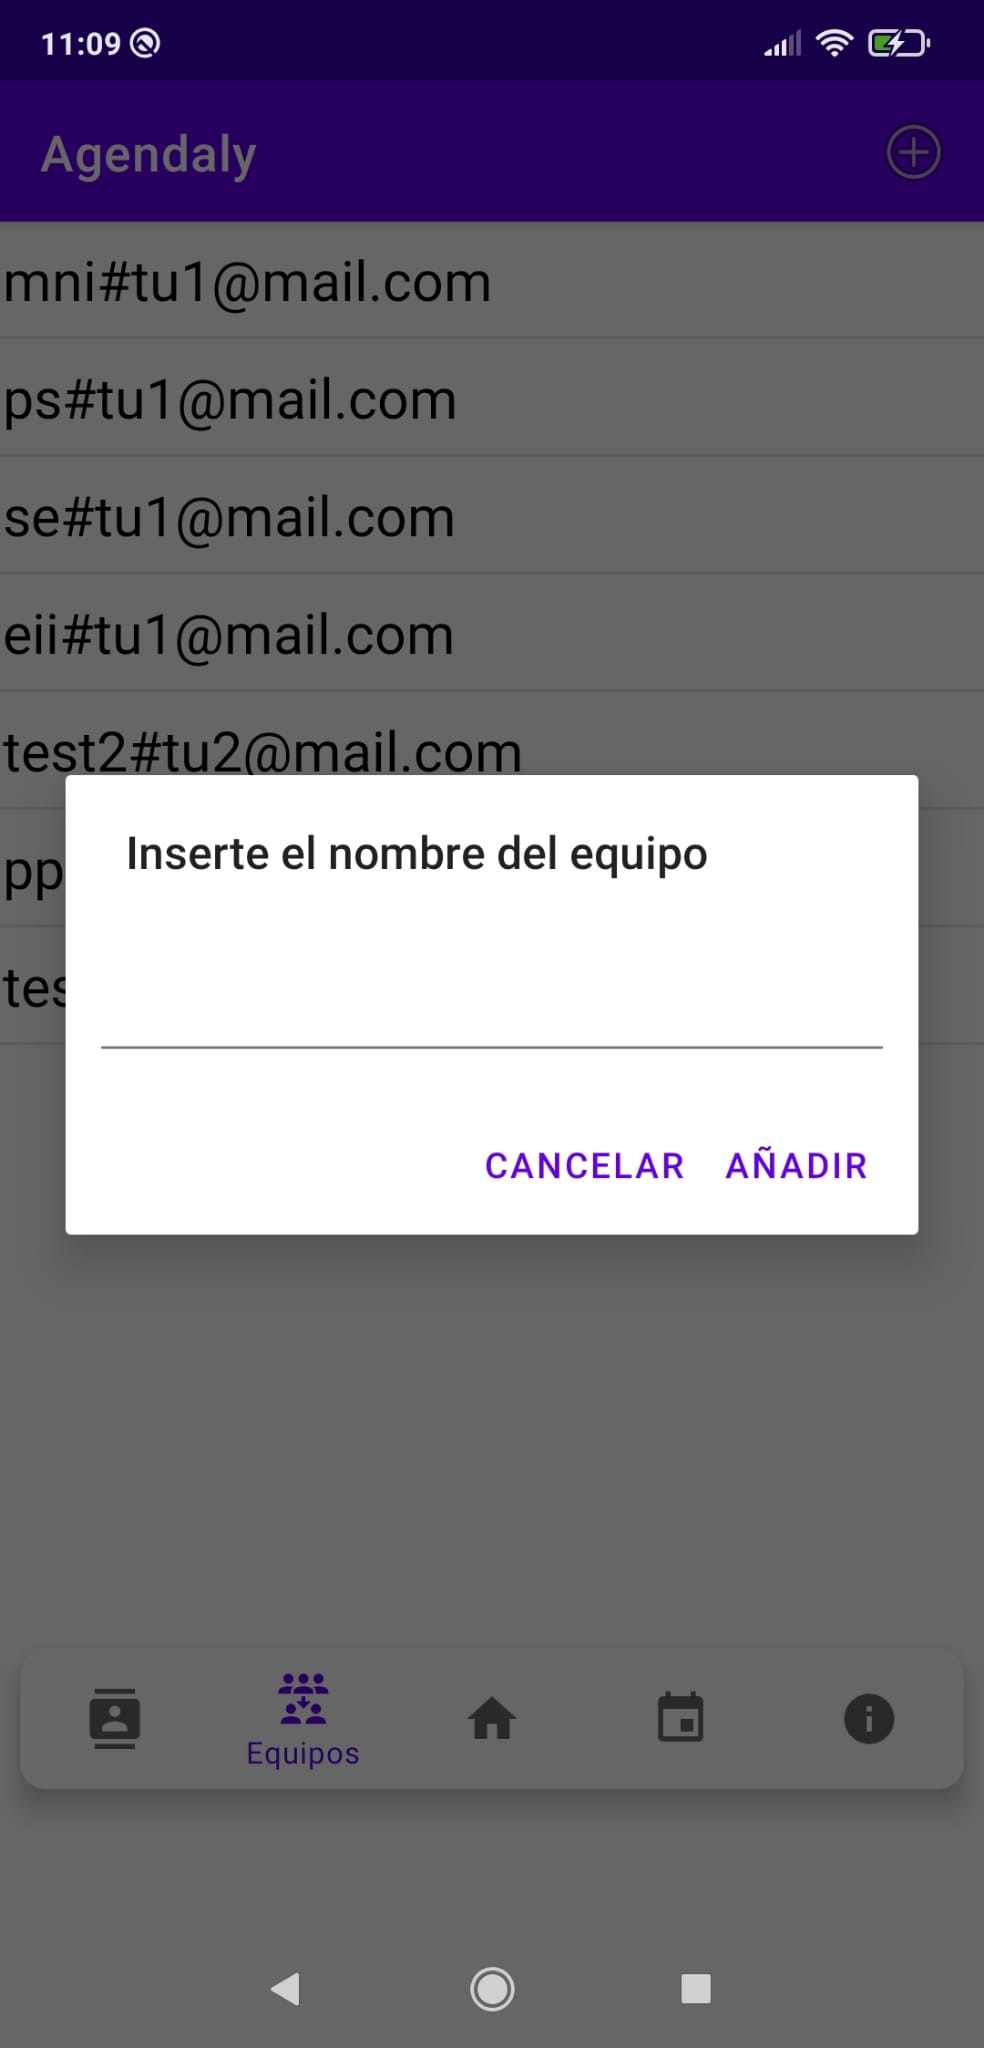
\includegraphics[scale=0.05]{add_team.jpeg}\hfill
    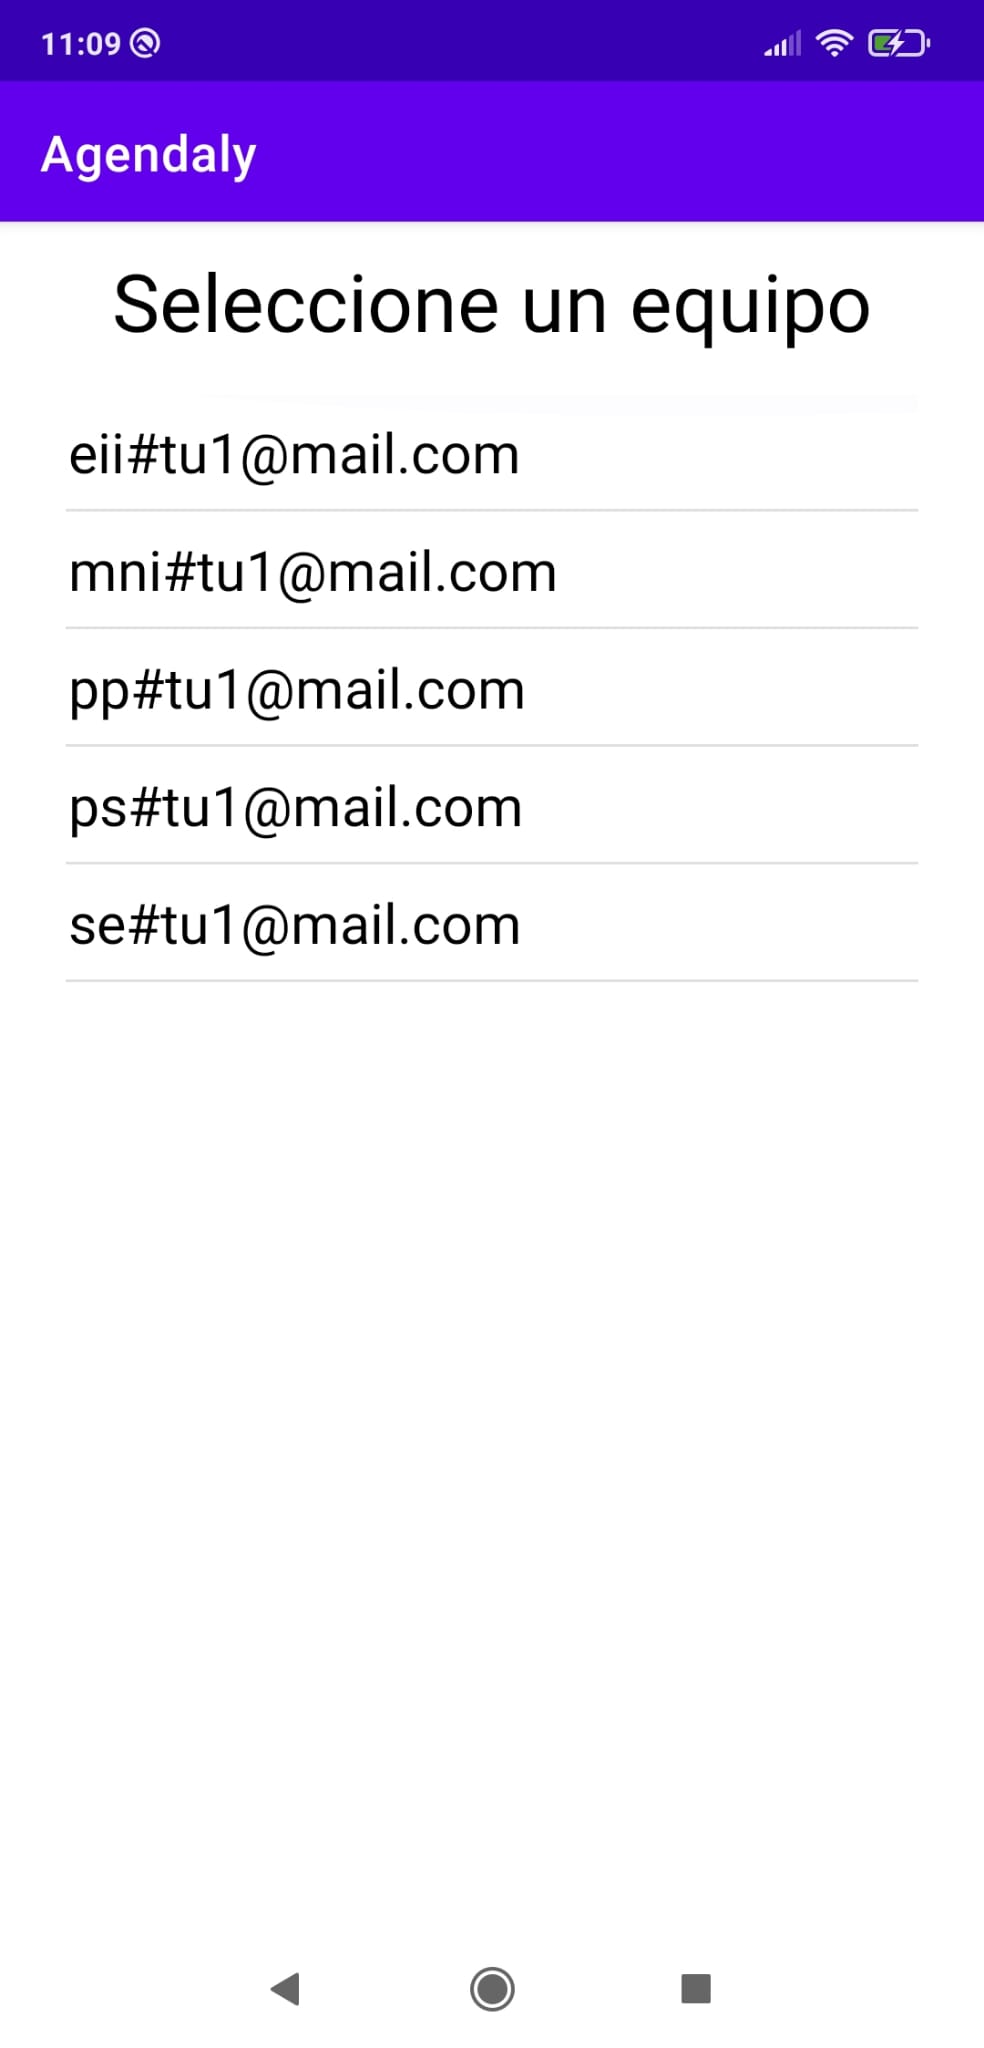
\includegraphics[scale=0.05]{add_to_Team.jpeg}\hfill
    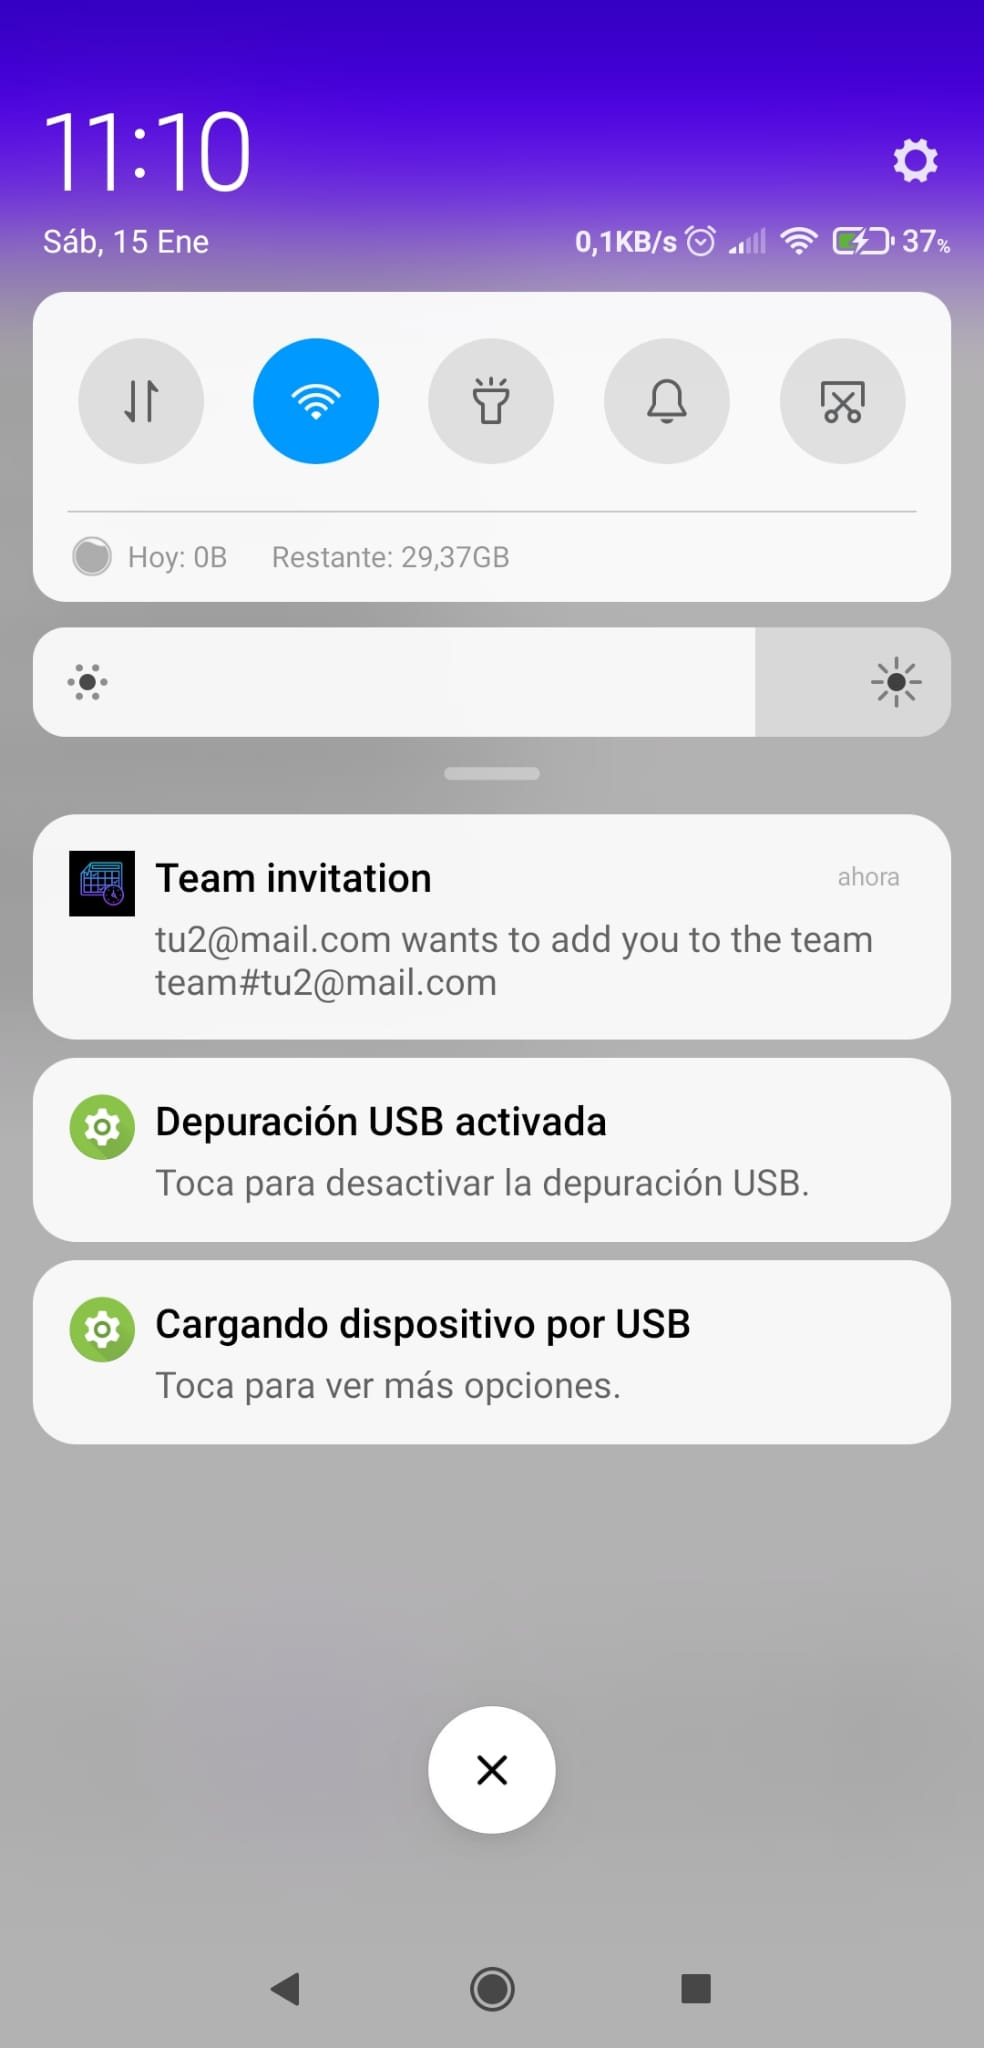
\includegraphics[scale=0.05]{notif_add_team.jpeg}\hfill
    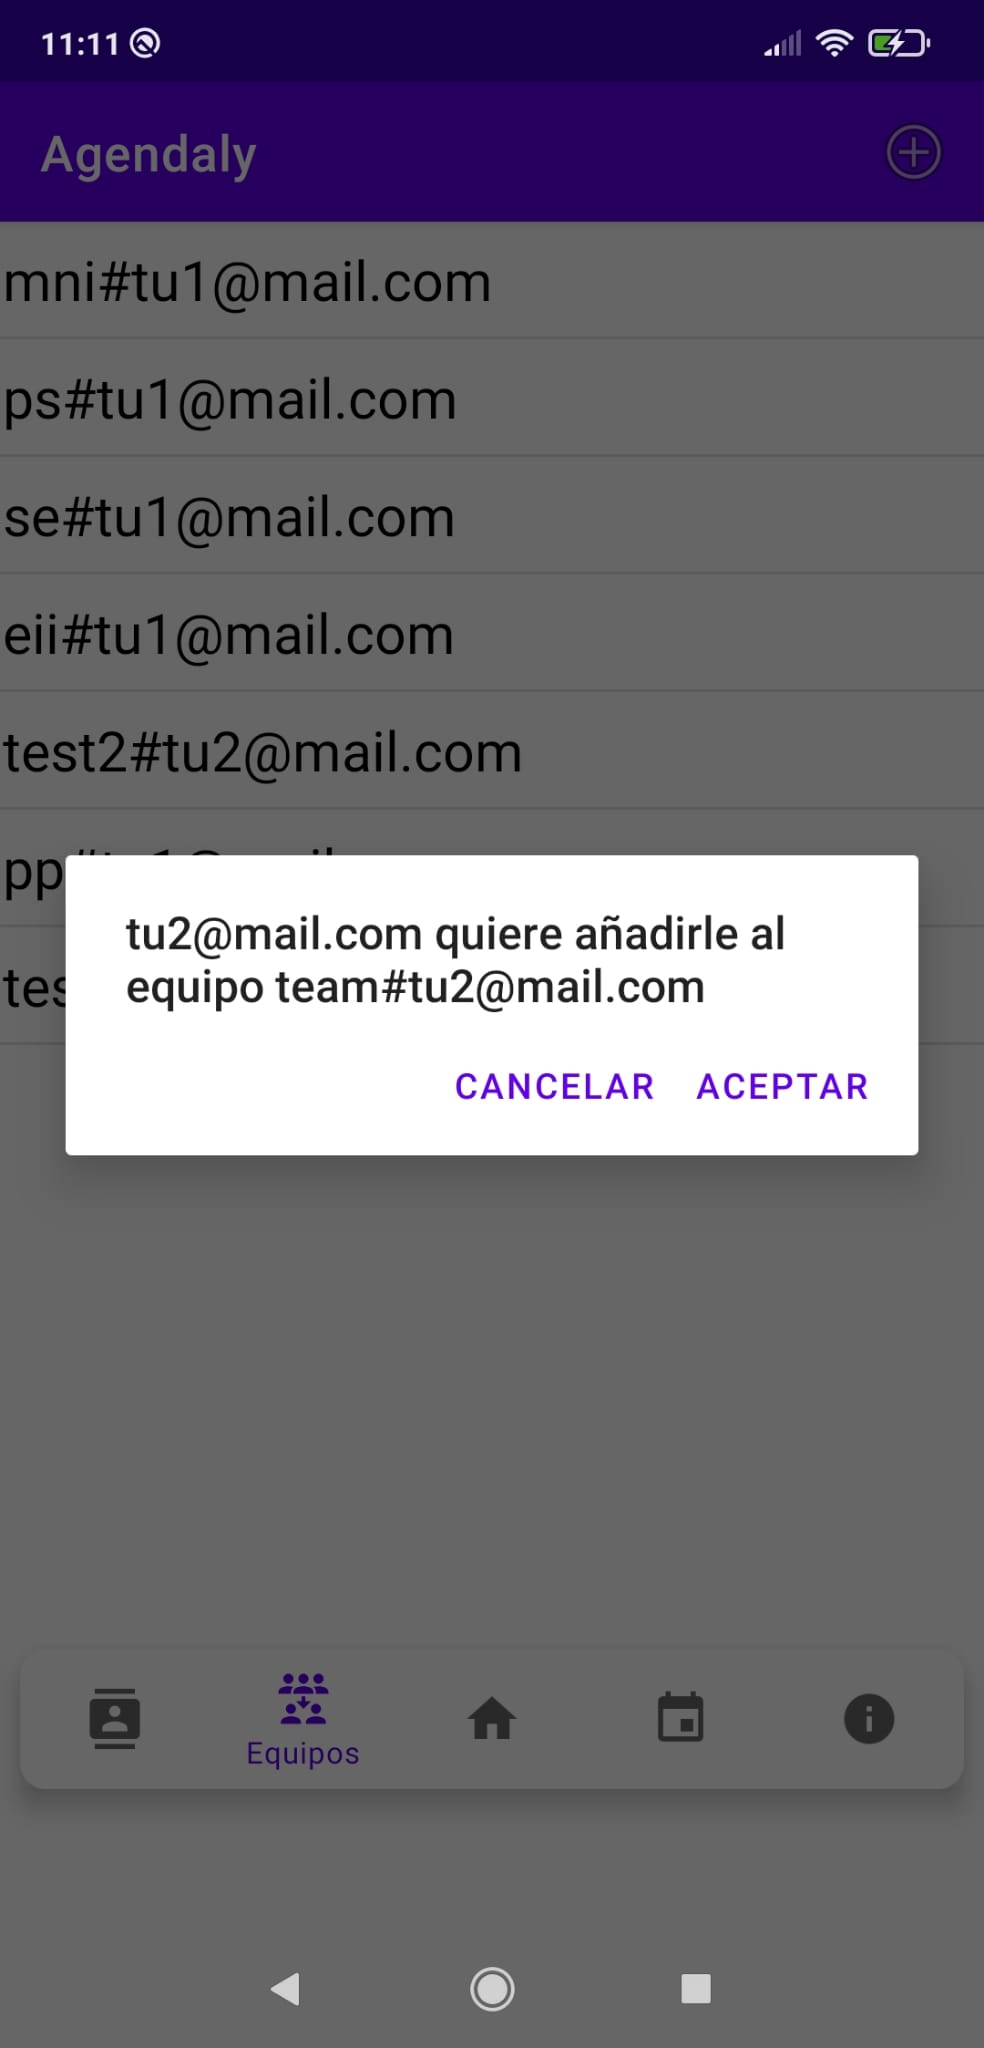
\includegraphics[scale=0.05]{addToTeamDialog.jpeg}\hfill
    \caption{Pantallas de contactos y equipos}
\end{figure}
\newpage

\subsection{Comunicaciones}
Las comunicaciones se pueden agrupar en tres tipos:
\begin{itemize}
    \item \textbf{de validación}: serán las que consulten al servidor en Firebase para procesos de autenticación o busca de usuarios.
    \item \textbf{de carga y almacenamiento de datos}: serán las que ejecuten operaciones CRUD contra la base de datos de Firestore.
    \item \textbf{peer2peer}: serán las que se realicen entre dispositivos utilizando los tokens de identificación y el API de Firebase Cloud Messaging.
\end{itemize}
\subsection{Sensores}
No aplica.
\subsection{Trabajo en background}
En el proceso de autenticación se realizan dos tareas: el propio inicio de sesión, el cual se valida contra el servidor de autenticación de Firebase; y el guardado del token de identificación de la sesión en la instalación. Este último es un valor alfanumérico que se guarda en una base de datos documental alojada en cloud, la cual permite el direccionamiento de las invitaciones a equipos entre dispositivos.
Para los casos de uso de contactos y equipos, se realizan operaciones en segundo plano que podemos agrupar en:
\begin{itemize}
    \item \textbf{Tareas de acceso a BD local}: todas las operaciones con contactos y equipos son guardadas localmente en una base de datos, permitiendo al usuario su consulta sin conexión. Este almacenamiento persistente está ligado al inicio de sesión, y se borra al cerrar sesión.
    \item \textbf{Tareas de acceso a BD remota}: todas las operaciones con contactos y equipos tienen copia en una base documental en cloud (Firestore). Los usuarios que inicien sesión dispondrán de copia de seguridad en red de contactos y equipos. Estos datos son permanentes y no dependen de si el usuario cierra sesión.
    \item \textbf{Envío de datos entre dispositivos}: para añadir contactos a los equipos, se envían datos en segundo plano para la comunicación entre los dispostivos donde se ejecutan ambas cuentas.
    \item \textbf{Receiver}: para poder atender las comunicaciones entre dispositivos, hay un receiver que estará a la escucha de comunicaciones entrantes. Si recibe alguna comunicación, notificará al usuario.
\end{itemize} 

En lo referente al horario las operaciones que se ejecutan en segundo plano son las siguiente:
\begin{itemize}
\item \textbf{Acceso y modificación de la BD local}: las operaciones para añadir y borrar asignaturas se realizan en segundo plano, así como las de lectura a la base datos. 
\item \textbf{Notificaciones programadas en el horario}: las notificaciones son programadas haciendo uso del Alarm Manager que las mandará en la hora que indicada y esta información será recogida por un Receiver el cual generará la notificación.

En cuanto al trabajo en background en relación con el calendario:

\item \textbf{Acceso y modificación de la BD local}: las operaciones para añadir y borrar eventos se realizan en segundo plano, así como las de lectura a la base datos.

\item \textbf{Notificaciones programadas en el horario}: para la implementación del envío de las notificaciones de los eventos con la antelación especificada por el usuario se ha utilizado Alarm Manager. De esta forma, Alarm Manager envía la información del evento tantos días antes como sea necesario, y a partir de esos datos el Receiver genera la notificación.
\end{itemize}


\section{Detalles de la implementación}
Estos se dividirán por tareas:
\begin{itemize}
    \item \textbf{Autenticación}: consta de dos actividades. La actividad AuthenticationActivity y ProfileActivity. En la primera se realiza el log in y el registro, y en la segunda el logout. Al iniciar la aplicación se intenta acceder automáticamente a partir de un fichero de SharedPreferences. Si el fichero está vacío, se le pide al usuario que se registre o inicie sesión. El registro sólo es posible si se usa una cuenta de Agendaly, mientras que si se utiliza Google el inicio de sesión está automáticamente linkado con Firebase. Una vez se realiza este proceso, se lanza la actividad Horario. 
    \newline
    Para el logout, se accede a la pestaña "Cuenta". En esa actividad se muestra información del usuario y un botón para hacer el logout. El proceso de logout es muy simple y funciona con y sin conexión, pues borra los datos locales de acceso, y ejecuta la activity AuthenticationActivity, volviendo a inicial el ciclo de funcionamiento de la aplicación.
    \newline
    En cuanto a la seguridad, la clase AuthUtils abstrae el manejo de usuarios y contraseñas locales, encargándose de guardar, eliminar y obtener datos de usuarios, así como de encriptar las contraseñas. Las contraseñas se guardan encriptadas para que no se puedan obtener manualmente mediante el sistema de ficheros de Android (en caso de dispositivos root o con USB Debug activado).
        
\end{itemize}

\begin{itemize}
    \item \textbf{Horario}: para implementar el horario se usan dos fragmentos y un bottom app bar. \newline
    El bottom appbar nos permite navegar entre el horario, el calendario y la información de usuario autentificado. \newline
    El primer fragmento nos muestra un calendario y el segundo el horario programado para ese día.
    Para el calendario se usa horizontal calendar\cite{misc-hc} que nos permite elegir el día y si mantenemos pulsado una fecha nos lleva al calendario general. \newline
    El segundo fragmento está formado por un Swipe, un TableLayout y un RecyclerView. El Swipe se usa para refrescar el recyclerView en el caso de que hayamos agregado o eliminado una asignatura y no cambiemos de día. El TableLayout nos explica la información que sale por el recyclerView. \newline 
    Las asignaturas se guardan en un base de datos, implementada con Room, guardando de ellas un id generado automáticamente, el nombre de la asignatura, el aula, el día, cuando empieza y cuando acaba. \newline
    Para añadir o eliminar asignaturas se usa un menu formado por dos iconos el + para añadir y un cubo de basura para borrar la asignatura.\newline
    En el momento de añadir una asignatura tendremos que rellenar dos EditText uno con el nombre de la asignatura y otro con el aula, elegir las horas de inicio y fin con un TimePicker para cada uno y por último seleccionar el día de la semana en un Spinner. Una vez cubierto le damos al botón que dice guardar y este guardará esta información en la base de datos local a la vez que nos muestra un Toast que nos dice que se ha guardado correctamente la asignatura.
    \newline
    A la hora de eliminar, tenemos que escribir en un EditText la asignatura a borrar y darle al botón que dice borrar. En ese momento saldrá un aviso para confirmar que vamos a borrar la asignatura mediante un cuadro de diálogo. Una vez aceptamos borraremos la asignatura de la base de datos local y sacará un Toast confirmando la operación.
    

\end{itemize}

\begin{itemize}
    \item \textbf{Notificaciones del Horario}:las notificaciones se implementan añadiendo en el menú del horario dos iconos más uno con forma de reloj sirve para especificar la hora a la que queremos que se nos notifique las asignaturas cada día, el otro con forma de campana que no servirá para activar o desactivar las notificaciones, si la campana está "apagada" no se podrán programar las notificaciones, si esta está activa se notificará con la hora guardada anteriormente. Si pulsamos se desactivara las notificaciones pero la hora programada seguirá guardada. 
    
\end{itemize}
\begin{itemize}
    \item \textbf{Calendario}:
    para el calendario se han creado inicialmente un LinearLayout con los botones de adelante y atrás y el nombre del mes, otro con los nombres de los días de la semana y un RecycledView donde irán los números de cada día del mes.  \newline
    Las fechas se organizan en seis filas y siete columnas dado que, en el peor de los casos (cuando un mes de 30 o 31 días comienza en fin de semana), puede ser necesario utilizar las seis filas para representar todos los días del mes. Se puede cambiar el mes que se visualiza por pantalla pulsando dos botones, para ir al anterior y al siguiente mes. Cada celda contiene únicamente el número del día que representa.  \newline
    Cuando se selecciona un día del mes, se lanza una nueva actividad que muestra los eventos planeados para ese día, cada uno en forma de 3 textos: el título del evento, la hora a la que va a tener lugar y una breve descripción del mismo. Para obtener los valores de estos campos para cada evento, se accede a la base de datos implementada en Room.  \newline
    En esta actividad también existe un menú que permite añadir y eliminar eventos. Si se selecciona la opción de añadir, se lanzará una nueva actividad con tres textos que se corresponden con los campos que almacena cada evento y un EditText por cada uno, para que los datos con los que se rellenen sean aquellos que se añaden a la base de datos para cada evento. También es posible configurar una notificación para el evento en esta pantalla.  Cuando se acaben de especificar estos campos, existe el botón de guardar, que añade el evento y los atributos introducidos a la base de datos. Por último, se vuelve a la pantalla principal del calendario y se mostrará un Toast en la parte inferior que verifica que el evento ha sido añadido correctamente. \newline
    Otra opción del menú que aparece cuando se abre el detalle de un día en concreto es el de eliminar un evento. Si se pulsa el icono de la papelera del menú, se lanza una nueva actividad con un editText en el que se podrá especificar el nombre del evento a eliminar, y a continuación borrarlo pulsando un botón.
    
\end{itemize}
\begin{itemize}
    \item \textbf{Notificaciones del calendario}:
    en el momento en el que se entre en la pantalla del calendario en se recibirán las notificaciones de los eventos en los que se haya elegido esta opción. \newline
    Las notificaciones se configuran en el momento de crear el evento. Hay un texto que indica la posibilidad de configurar la notificación de ese evento, y para ello también hay un editText donde se podrá incluir el número de días de antelación con los que se desea recibir la notificación del evento, y un switch que activa o desactiva esta opción. \newline
    El usuario puede modificar en cualquier momento tanto el número de días de antelación de las notificaciones como la activación o desactivación de las notificaciones de cada evento individualmente. 
\end{itemize}
    
\begin{itemize}
    \item \textbf{Contactos y equipos}: en ambos casos se dispone de un conjunto RecyclerView + Menús / Menú contextual. A través del menú contextual se abrirán los diálogos de entrada de datos, los cuales permitirán añadir nuevos contactos, añadir nuevos equipos o invitar contactos a equipos de propia creación. En ambos casos la persistencia se maneja con bases de datos locales (para acceso sin conexión), pero la funcionalidad completa requiere de conexión a internet (puesto que estos datos se guardan en una base de datos remota y se necesita comunicación entre dispositivos para enviar las invitaciones de participación). La actualización del RecyclerView se realiza automáticamente al terminar las operaciones CRUD sobre las bases de datos (locales y remotas).
    \item \textbf{Notificaciones de invitaciones}: en este caso se crea una notificación que al ser pulsada despliega un diálogo de confirmación. Si el usuario acepta unirse al equipo, el equipo se añadirá local y remotamente. Después se actualizará la vista del recycler view de la activity Teams asíncronamente.
\end{itemize}

%%%%%%%
%%%%%%%
\section{Pruebas realizadas y evaluación de las mismas}
Las pruebas realizadas han sido pruebas manuales. No disponemos de test automatizados de unidad, integración ni aceptación.
\newline
En cuanto a las pruebas manuales, varían según la funcionalidad implementada:
\begin{itemize}
    \item \textbf{Autenticación}: se comprobó el inicio e cierre de sesión, los datos de los ficheiros de preferencias compartidas y la generación de los tokens para comunicaciones con ambos métodos de autenticación.
    \item \textbf{Contactos}: se comprobó que sólo se pudiesen añadir contactos registrados en Agendaly, así como que añadiesen correctamente. Se comprobó también si los datos se recuperan automáticamente al iniciar sesión y si se borraran de la base de datos local al cerrar sesión.
    \item \textbf{Equipos}: se comprobó que se pudiesen añadir equipos propios, así como que se añadieran los provenientes de invitación. También se comprobó que los datos se recuperaran automáticamente al iniciar sesión y se borraran de la base de datos local al cerrar sesión.
    \item \textbf{Invitaciones y notificaciones}: se comprobó el envío de datos entre dispositivos, la recepción y la creación de las notificaciones.
    \item \textbf{Calendario}: se ha probado a ir y volver desde las diferentes pantallas de la aplicación a la pantalla principal del calendario. También que se pueda cambiar de mes y que se visualiza correctamente en cualquier caso: meses de 28, 29, 30 y 31 días, que encajen con los días de la semana correspondientes comprobandolo con un calendario real. Se comprobó que se pueden crear eventos, siempre que tengan un nombre (no son necesarios el resto de los campos). Se ha confirmado que se pueden borrar eventos de tal forma que tras haber sido borrados no aparecen en el día en el que se habían creado, ni se recibe la notificación en caso de haber sido activada.
    \item \textbf{Notificaciones del calendario}: se ha verificado que al entrar en la pantalla del calendario se reciben las notificaciones de los eventos en los que se han configurado. Se ha comprobado que cambiando la antelación de las notificaciones se siguen recibiendo. Se ha confirmado que no es posible introducir caracteres que no sean números naturales en el editText a la hora de establecer la notificación. Se ha probado que una vez se ha eliminado un evento cuya notificación estaba activada, no se vuelve a recibir al entrar en la pantalla del calendario.

    \item \textbf{Horario}: se ha probado ha añadir diferentes asignaturas y a añadirlas sin algunos de los campos. Borrar estas asignaturas. 
    
    \item \textbf{Notificaciones de horario}: se ha probado a que enviara notificaciones estableciendo una hora cercana en ese mismo día, estableciendo este mismo tiempo y cambiando de día para que notifique las asignaturas de ese día a esa misma hora teniendo en cuenta que si no hay asignaturas no notifique. También se ha probado a establecer una notificación y desactivarla acto seguido para comprobar que no se manda cuando se desactiva. Y también se ha comprobado que si la "campana está desactivada" no se podrán establecer notificaciones.

\end{itemize}
\section{Trabajo futuro}
Se establecerá por funcionalidad:
\begin{itemize}
    \item \textbf{Autenticación}: añadir proveedores de inicio de sesión.
    \item \textbf{Contactos y equipos}: añadir completo manejo sobre todos los parámetros de contactos y equipos. Concretamente, con respecto a los equipos, añadir roles, configuraciones de equipos, gestionar tareas grupales, asignar tareas a integrantes de los equipos, sincronizar los datos de equipos entre participantes y permitir almacenamiento de documentos conjuntos. Con respecto a las notificaciones, añadir mailboxes que permitan mantenerlas en espera, así como volver a verlas posteriormente, mejorando el sistema de comunicación distribuída entre dispositivos. Mejoras de interfaz y user experience.
    
    \item \textbf{Horario}: mejorar la interfaz y permitir añadir más características a la hora de guardar información sobre las asignaturas así como a la hora de lo que se muestra por pantalla. 
    
    \item \textbf{Notificaciones de horario}: añadir más personalización a las notificaciones como por ejemplo poder posponerla para que te avise más adelante en ese mismo día o desactivar los avisos desde la misma.
    
    \item \textbf{Calendario}: Se podrían añadir diferentes formas de visualizar los días en el calendario: formato semanal y anual, también mejoras menores en la interfaz a la hora de visualizar los eventos de un día seleccionado y mejoras en la usabilidad.
    
    \item \textbf{Notificaciones del calendario}: una posible mejora sería profundizar en el diseño de las notificaciones y que contasen con una opción de "posponer", o al pulsar sobre ellas llevasen al usuario a la pantalla de edición.
    
    
\end{itemize}
\section{Incidencias destacables en la realización del TT}
A nivel general no hemos tenido prácticamente problemas porque las partes están bastante compartimentadas.
Podemos agrupar las incidencias por funcionalidad:
\begin{itemize}
    \item \textbf{Autenticación}: no hubo incidencias relevantes.
    \item \textbf{Contactos y equipos}: la gestión de dos sistemas de almacenamiento (local y distribuido) complica la sincronización de los datos. Necesidad de depender de proveedores externos para la gestión de datos y comunicación multiusuario. Esta dependencia complica toda la lógica de negocio del sistema. En futuras versiones se debería invertir tiempo en la construcción de un servidor con acceso a bases de datos propias que permitiera: (1) simplificar la lógica de negocio sustituyendo el API de Firebase por un API REST estándar, en el cual no hubiera que restringir el funcionamiento a los formatos de envío de información que Google nos proporciona; y (2) dejar de depender de proveedores de servicios externos, permitiendo una mejor escalabilidad, así como permitirnos pruebas automatizadas con un desarrollo e integración contínua de producto que no devenguen en gastos de cloud. 
    Además, el no depender de proveedores nos posibilitaría para la migración de la comunicación, para que sea basada en servidor, y no peer to peer, mejorando y simplificando el manejo de notificaciones (sobre todo en primer plano). Este mecanismo nos permitiría manejar todas las notificaciones con un "mailbox" de servidor, de modo que ninguna se perdiese (incluso si el usuario simplemente se deshacía de ellas).

    \item \textbf{Horario}: no hubo incidencias mayores más allá de la gestión adecuada de los fragmentos para que hubiera una sincronización entre el día y la información.
    
    \item \textbf{Calendario}: a la hora de crear un evento, en la base de datos se almacena también la fecha en la que tendrá lugar. Esta información no se recibe por medio de un editText que rellena el usuario (como ocurre con el resto de campos), si no que va implícita en el momento en el que se selecciona el día en el que se crea el evento. Fue necesario transformar la fecha a una cadena de caracteres para que fuese posible almacenarla en la base de datos.

    \item \textbf{Notificaciones del horario y del calendario}: para implementar estas funciones se tuvo que modificar los datos guardados en la BD generando esto errores a la hora de los datos guardados anteriormente y lo que se quería guardar ahora, para solucionar esto se optó por borrar los datos almacenados hasta el momento.



\end{itemize}
Debido a falta de tiempo, no se han podido terminar de completar algunas funcionalidades, más concretamente, la organización de equipos (hay una funcionalidad básica pero la completa requeriría más tiempo e infraestructura) y el repositorio de apuntes (para el cual necesitaríamos mucho almacenamiento en cloud, además de que sería un proyecto de expansión tan grande o más que la propia aplicación).\newpage

\bibliographystyle{pfc-fic}
\bibliography{biblio}
\addcontentsline{toc}{section}{Bibliografía}

\end{document}
